% -*- mode: LaTeX; TeX-PDF-mode: t; -*-
\documentclass[BufferStockTheory]{subfiles}
% WARNING: Different AucTeX execution depending on whether
% 0. Being compiled as standalone document
%    * Compile this file, then main, then this one again
%    * Keep iterating until neither file changes
% 0. Being compiled as subfile of main document
%    * Just compile main document repeatedly

\providecommand{\econtexRoot}{}
\renewcommand{\econtexRoot}{..}
\providecommand{\econtexPaths}{}\renewcommand{\econtexPaths}{\econtexRoot/Resources/econtexPaths}
% The \commands below are required to allow sharing of the same base code via Github between TeXLive on a local machine and Overleaf (which is a proxy for "a standard distribution of LaTeX").  This is an ugly solution to the requirement that custom LaTeX packages be accessible, and that Overleaf seems to ignore symbolic links (even if they are relative links to valid locations)
\providecommand{\econtex}{\econtexRoot/Resources/texmf-local/tex/latex/econtex}
\providecommand{\econtexSetup}{\econtexRoot/Resources/texmf-local/tex/latex/econtexSetup}
\providecommand{\econtexShortcuts}{\econtexRoot/Resources/texmf-local/tex/latex/econtexShortcuts}
\providecommand{\econtexBibMake}{\econtexRoot/Resources/texmf-local/tex/latex/econtexBibMake}
\providecommand{\econtexBibStyle}{\econtexRoot/Resources/texmf-local/bibtex/bst/econtex}
\providecommand{\econtexBib}{economics}
\providecommand{\notes}{\econtexRoot/Resources/texmf-local/tex/latex/handout}
\providecommand{\handoutSetup}{\econtexRoot/Resources/texmf-local/tex/latex/handoutSetup}
\providecommand{\handoutShortcuts}{\econtexRoot/Resources/texmf-local/tex/latex/handoutShortcuts}
\providecommand{\handoutBibMake}{\econtexRoot/Resources/texmf-local/tex/latex/handoutBibMake}
\providecommand{\handoutBibStyle}{\econtexRoot/Resources/texmf-local/bibtex/bst/handout}

\providecommand{\FigDir}{\econtexRoot/Figures}
\providecommand{\CodeDir}{\econtexRoot/Code}
\providecommand{\DataDir}{\econtexRoot/Data}
\providecommand{\SlideDir}{\econtexRoot/Slides}
\providecommand{\TableDir}{\econtexRoot/Tables}
\providecommand{\ApndxDir}{\econtexRoot/Appendices}

\providecommand{\ResourcesDir}{\econtexRoot/Resources}
\providecommand{\rootFromOut}{..} % Path back to root directory from output-directory
\providecommand{\LaTeXGenerated}{\econtexRoot/LaTeX} % Put generated files in subdirectory
%\providecommand{\EqDir}{\econtexRoot/Equations} % Put generated files in subdirectory
\providecommand{\EqDir}{Equations} % Put generated files in subdirectory
\providecommand{\econtexPaths}{\econtexRoot/Resources/econtexPaths}
\providecommand{\LaTeXInputs}{\econtexRoot/Resources/LaTeXInputs}
\providecommand{\LtxDir}{LaTeX/}


\onlyinsubfile{% https://tex.stackexchange.com/questions/463699/proper-reference-numbers-with-subfiles
    \csname @ifpackageloaded\endcsname{xr-hyper}{%
      \externaldocument{\econtexRoot/BufferStockTheory}% xr-hyper in use; optional argument for url of main.pdf for hyperlinks
    }{%
      \externaldocument{\econtexRoot/BufferStockTheory}% xr in use
    }%
    \renewcommand\labelprefix{}%
    % Initialize the counters via the labels belonging to the main document:
    \setcounter{equation}{\numexpr\getrefnumber{\labelprefix eq:Dummy}\relax}% eq:Dummy is the last number used for an equation in the main text; start counting up from there
}


\onlyinsubfile{\externaldocument{BufferStockTheory}} % Get xrefs -- esp to appendix -- from main file; only works properly if main file has already been compiled;

\begin{document}

% Attempted to make all lines used for Web version contain {Web} (or version with only single curly brace at end) so can be removed with sed
\providecommand{\versn}{pdf} % Version; like, web or pdf or journal submission
\ifthenelse{\boolean{Web}}{    % {Web}
  \renewcommand{\versn}{Web}     % Too hard to figure out passing -output-directory through make4ht through htlatex, so web version is compiled with junk files in main directory
  \renewcommand{\rootFromOut}{.} % {Web}
}{}  % {Web}

% Tiny info header at top to track git commit
\hfill{\tiny \jobname~\versn~\today~{at} \DTMcurrenttime, \input{\ResourcesDir/.git-source-commit}~~\input{\ResourcesDir/.git-public-commit}}

\title{Theoretical Foundations of \\ Buffer Stock Saving}

\author{Christopher D. Carroll\authNum}

\keywords{Precautionary saving, buffer stock saving, marginal propensity to consume, permanent income hypothesis, income fluctuation problem}

\jelclass{D81, D91, E21 \par
  \href{https://econ-ark.org}{
\includegraphics{\ResourcesDir/PoweredByEconARK}}
}

\renewcommand{\forcedate}{September 17, 2021}\date{\forcedate}

\maketitle
\hypertarget{abstract}{}
\begin{abstract}
This paper builds foundations for rigorous and intuitive understanding of `buffer stock' saving models (\cite{bewleyPIH}-like models with a wealth target), pairing each theoretical result with quantitative illustrations.  After describing conditions under which a consumption function exists, the paper articulates stricter `Growth Impatience' conditions that guarantee alternative forms of stability --- either at the population level, or for individual consumers.  Together, the numerical tools and analytical results constitute a comprehensive toolkit for understanding buffer stock models.
\end{abstract}


% Various resources
\hypertarget{links}{}

\begin{footnotesize}
  \parbox{0.9\textwidth}{
    \begin{center}
      \begin{tabbing}
          \texttt{Dashboard:~} \= \= \texttt{\url{https://econ-ark.org/materials/BufferStockTheory?dashboard}} \\
          \texttt{~~~REMARK:~} \> \> \texttt{\url{https://econ-ark.org/materials/BufferStockTheory}} \\ % Owner is defined in Resources/owner.tex
          \texttt{~~~~~html:~} \> \> \texttt{\href{https://\owner.github.io/BufferStockTheory/}{https://\owner.github.io/BufferStockTheory/}} \\ % Owner is defined in Resources/owner.tex
          \texttt{~~~~~~PDF:~} \> \> \texttt{\href{https://\owner.github.io/BufferStockTheory/BufferStockTheory.pdf}{https://\owner.github.io/BufferStockTheory/BufferStockTheory.pdf}} \\ % Owner is defined in Resources/owner.tex
          \texttt{~~~Slides:~} \> \> \texttt{\href{https://\owner.github.io/BufferStockTheory/BufferStockTheory-Slides.pdf}{https://\owner.github.io/BufferStockTheory/BufferStockTheory-Slides.pdf}} \\
          \texttt{~Appendix:~} \> \> \texttt{\href{https://\owner.github.io/BufferStockTheory\#Appendices}{https://\owner.github.io/BufferStockTheory\#Appendices}}    \\
          \texttt{~~~GitHub:~} \> \> \texttt{\href{https://github.com/\owner/BufferStockTheory}{https://github.com/\owner/BufferStockTheory}} \\
      \end{tabbing}
    \end{center}
    The \href{https://econ-ark.org/materials/BufferStockTheory?dashboard}{dashboard} lets users see consequences of alternative parameters in an interactive framework.} % end parbox{\textwidth}
\end{footnotesize}

\begin{authorsinfo}
  \name{Contact: \href{mailto:ccarroll@jhu.edu}{\texttt{ccarroll@jhu.edu}}, Department of Economics, 590 Wyman Hall, Johns Hopkins University, Baltimore, MD 21218, \url{https://www.econ2.jhu.edu/people/ccarroll}, and National Bureau of Economic Research.}
\end{authorsinfo}

\newcommand{\thankstext}{
  The paper's results \href{https://\owner.github.io/nbreproduce}{can be automatically reproduced} using the \href{https://econ-ark/HARK}{Econ-ARK/HARK} toolkit, which can be cited per our references (\cite{carroll_et_al-proc-scipy-2018}); for reference to the toolkit itself see \href{https://econ-ark.org/acknowledging/}{Acknowleding Econ-ARK}.  Thanks to the \href{https://consumerfinance.gov}{Consumer Financial Protection Bureau} for funding the original creation of the \href{https://econ-ark.org}{Econ-ARK} toolkit; and to the \href{https://sloan.org}{Sloan Foundation} for funding Econ-ARK's \href{https://sloan.org/grant-detail/8071}{extensive further development} that brought it to the point where it could be used for this project.  The toolkit can be cited with its digital object identifier, \href{https://doi.org/10.5281/zenodo.1001067}{10.5281/zenodo.1001067}, as is done in the paper's own references as \cite{carroll_et_al-proc-scipy-2018}.  Thanks to Will Du, James Feigenbaum, Joseph Kaboski, Miles Kimball, Qingyin Ma, Misuzu Otsuka, Damiano Sandri, John Stachurski, Adam Szeidl, Alexis Akira Toda, Metin Uyanik, Mateo Vel\'asquez-Giraldo, Weifeng Wu,  Jiaxiong Yao, and Xudong Zheng for comments on earlier versions of this paper, John Boyd for help in applying his weighted contraction mapping theorem, Ryoji  Hiraguchi for extraordinary mathematical insight that improved the  paper greatly, David Zervos for early guidance to the literature, and participants in a seminar at the Johns Hopkins University, a presentation at the 2009 meetings of the Society of Economic Dynamics for their insights, and at a presentation at the Australian National University.}

\ifthenelse{\boolean{Web}}{}{
  \begin{minipage}{0.9\textwidth}
    \tiny \thankstext
\end{minipage}
} % {Web}
{\titlepagefinish}

\hypertarget{Introduction}{}
\section{Introduction}\label{sec:intro}

In the presence of realistic transitory and permanent shocks to income \textit{a la}~\cite{friedmanATheory} and~\cite{muthOptimal}, only one further ingredient is required to construct a microeconomically testable model of consumption: A description of preferences.  Zeldes~\citeyearpar{zeldesStochastic} was the first to calibrate a quantitatively plausible example; his paper spawned a literature showing that such models' predictions can match household life cycle data reasonably well, whether or not explicit liquidity constraints are imposed.\footnote{See~\cite{carrollBSLCPIH} or~\cite{gpLifeCycle} for arguments that models with only `natural' constraints (see below) match a wide variety of facts; for a model with explicit constraints that produces very similar results, see, e.g.,~\cite{Cagetti}.}

A connected literature in macroeconomic theory, starting with~\cite{bewleyPIH}, has derived limiting properties of related infinite-horizon problems, but only in models more complex than the case with just shocks and preferences. The extra complexity has been imposed because standard contraction mapping theorems (beginning with~\cite{bellmanDynamicProgramming} and including those building on Stokey et~al.~\citeyearpar{slpMethods}) cannot be applied when utility and/or marginal utility are unbounded. Many proof methods also rule out permanent shocks \textit{a la}~\cite{friedmanATheory},~\cite{muthOptimal}, and~\cite{zeldesStochastic}.\footnote{See \hyperlink{DiffFromLit}{the fuller discussion} at the end of Section~\ref{subsec:Setup}.}

This paper's first technical contribution is to articulate conditions under which the infinite-horizon version of the Friedman-Muth-Zeldes problem (without complications like a consumption floor or liquidity constraints) defines a contraction mapping whose limiting solution is sensible as the horizon approaches infinity.  A \hyperlink{FVAC}{`Finite Value of Autarky Condition'} is mostly sufficient (the other imposed condition, the \hyperlink{WRIC}{`Weak Return Impatience Condition'},\footnote{This is a generalization of a condition in~\cite{mstIncFluct}.} is unlikely to bind).  Because the infinite horizon solution is the limit of finite-horizon recursions, many intermediate results are also useful for solving finite-horizon problems.

But the paper's main theoretical contribution is to identify, for the infinite-horizon case, conditions under which `stable' values of the wealth-to-permanent-income ratio exist, either for individual consumers (a consumer's wealth can be predicted to move toward a `target' ratio) or for the aggregate (the economy as a whole moves toward a `balanced growth' equilibrium).  The requirement for stability is always that the model's parameters satisfy a `Growth Impatience Condition' whose details depend on the quantity whose stability is of interest.  A model that exhibits stability of either kind qualifies as a `buffer stock' model.\footnote{Such models are neither a subset nor a superset of~\cite{bewleyPIH} models.  But closed economies in which capital results from saving and has declining marginal productivity are always `buffer stock' economies under some definition of that term, because capital accumulation causes interest rates to fall, which guarantees that a Growth Impatience Condition will hold in equilibrium (see below).  The more interesting applications are to populations (or economies) whose marginal saving behavior does not determine the relevant interest rate, or in which the marginal product of capital does not fall as capital is accumulated (again, see below).}

\hypertarget{KMP}{} Even without a formal proof of its existence, buffer stock saving has been intuitively understood to underlie central quantitative results in heterogeneous agent macroeconomics; for example, the logic of target saving is central to the claim by~\cite{kmpHandbook} in the \textit{Handbook of Macroeconomics} that such models explain why, during the Great Recession, middle-class consumers cut their spending more than the poor or the rich.  The theory below provides the rigorous basis for this claim:  Learning that the future has become more uncertain does not change the urgent imperatives of the poor (their high $\uFunc^{\prime}(\cRat)$ means they --- optimally --- have little room to maneuver).  And, increased labor income uncertainty does not much change the behavior of the rich because it poses little risk to their consumption.  Only people in the middle have both the motivation and the wiggle-room to respond by reducing their spending.

Analytical derivations for the proofs also explain many other results familiar from the numerical literature.

The paper begins by defining sufficient conditions for the problem to define a useful (nondegenerate) limiting consumption function (and explains how the model relates to those previously considered).  The conditions are interestingly parallel to those required for the \hyperlink{Factors-Defined-And-Compared}{liquidity constrained perfect foresight model}; that parallel is explored and explained.  This analysis establishes limiting properties of the consumption function as resources approach infinity, and as they approach their lower bound; using these limits, the contraction mapping theorem is proven.

The next theoretical contribution demonstrates that a corresponding model with an `artificial' liquidity constraint (a model that prohibits borrowing, even by consumers who could certainly repay) is a limiting case of the model without constraints. The analytical appeal of the unconstrained model is that it is both mathematically convenient (e.g., the consumption function is twice continuously differentiable), and arbitraily close (cf.\ Section~\ref{sec:deatonIsLimit}) to less tractable models. The idea is to prove a proposition in a congenial environment, then to define the analogous proposition as holding (in the limit) if it holds for in the limit as the horizon extends to infinity.

 In proving the remaining theorems, the \hyperlink{AnalysisoftheConvergedConsumptionFunction}{next section} examines the key properties of the model. First, as \hyperlink{LimitsAsmtToInfty}{cash approaches infinity} the expected growth rate of consumption and the marginal propensity to consume (MPC) converge to their values in the perfect foresight case. Second, as \hyperlink{LimitsAsmtToZero}{cash approaches zero} the expected growth rate of consumption approaches infinity, and the MPC approaches a simple analytical limit.  Next, the central theorems articulate conditions under which different measures of `growth impatience' imply useful conclusions about points of stability (`target' or `balanced growth' points).

The final section elaborates the conditions under which, even with a fixed aggregate interest rate that differs from the time preference rate, a small open economy populated by buffer stock consumers has a balanced growth equilibrium in which growth rates of consumption, income, and wealth match the exogenous growth rate of permanent income (equivalent, here, to productivity growth). In the terms of~\cite{schmitt2003closing}, buffer stock saving is an appealing method of `closing' a small open economy model, because it requires no ad-hoc assumptions.  Not even liquidity constraints.\footnote{The paper's insights are instantiated in the \href{https://econ-ark.org}{Econ-ARK} toolkit, whose \href{https://hark.readthedocs.io/en/stable/reference/ConsumptionSaving/ConsIndShockModel.html}{buffer stock saving module} flags parametric choices under which a problem is degenerate or under which stable ratios of wealth to income may not exist.}


\hypertarget{The-Problem}{}

\section{The Problem}

\subsection{Setup}\label{subsec:Setup}

The infinite horizon solution is the (limiting) first-period solution to a sequence of finite-horizon problems as the horizon (the last period of life) becomes arbitrarily distant.

That is, for the value function, fixing a terminal date $T$,  we are interested in the term $\vLevBF_{T-n}$ in the sequence of value functions $\{\vLevBF_{T},\vLevBF_{T-1},\ldots,\vLevBF_{T-n}\}$.  We will say that the problem has a `nondegenerate' infinite horizon solution if, corresponding to that $\vLevBF$, as $n \uparrow \infty$ there is a limiting consumption function $\usual{\cFunc}(\mRat) = \lim_{n \uparrow \infty} \cFunc_{T-n}$ which is neither $\usual{\cFunc}(\mRat)=0$ everywhere (for all $\mRat$) nor $\usual{\cFunc}(\mRat)=\infty$ everywhere.

Concretely, a consumer born $n$ periods before date $T$ solves the problem
\begin{verbatimwrite}{\EqDir/supfn}
  \begin{align*}%    \label{eq:supfn}
    \vLevBF_{T-n} & = \max~ \Ex_{t}\left[\sum_{i=0}^{n} \DiscFac^{i} \uFunc(\cLevBF_{t+i})\right]
  \end{align*}
\end{verbatimwrite}
  \begin{align*}    \label{eq:supfn}
    \vLevBF_{T-n} & = \max~ \Ex_{t}\left[\sum_{i=0}^{n} \DiscFac^{i} \uFunc(\cLevBF_{t+i})\right]
  \end{align*}

where the Constant Relative Risk Aversion (CRRA) utility function
\begin{align}
  \uFunc(\bullet)=\bullet^{1-\CRRA}/(1-\CRRA) \label{eq:crrautil}
\end{align}
exhibits relative risk aversion $\CRRA > 1$.\footnote{The main
  results also hold for logarithmic utility which is the limit as
  $\CRRA \rightarrow 1$ but incorporating the logarithmic special case
  in the proofs is omitted because it would be cumbersome.}  The consumer's initial condition is
defined by market resources $\mLevBF_{t}$ and permanent noncapital income $\pLevBF_{t}$, which
both are positive,
\begin{align}
  \{\pLevBF_{t},\mLevBF_{t}\} & \in (0,\infty) \label{eq:pLevBFandmLevBFgt0},
\end{align}
and the consumer cannot die in debt,
\begin{align}
  \cLevBF_{T} & \leq  \mLevBF_{T} \label{eq:NoDebtAtDeath}.
\end{align}

\hypertarget{checkRestrictions}{}


In the usual treatment, a dynamic budget constraint (DBC) incorporates
several elements that jointly determine next period's $\mLevBF$ (given this
period's choices); for the detailed analysis here, it will be useful to
disarticulate and describe the steps:\hypertarget{DBCParts}{}
\begin{verbatimwrite}{\EqDir/DBCparts}
  \begin{align}
    \aLevBF_{t}    & = \mLevBF_{t}-\cLevBF_{t}  \label{eq:DBCparts} \\
    \kLevBF_{t+1}   & = \aLevBF_{t} \notag \\
    \bLevBF_{t+1}    & = \kLevBF_{t} \Rfree \notag \\
    \pLevBF_{t+1}  & = \pLevBF_{t} \underbrace{\PGro\pShk_{t+1}}_{\equiv \PGro_{t+1}}  \notag \\
    \mLevBF_{t+1}  & =  \bLevBF_{t+1} +\pLevBF_{t+1}\tShkAll_{t+1},  \notag
  \end{align}
\end{verbatimwrite}
  \begin{align}
    \aLevBF_{t}    & = \mLevBF_{t}-\cLevBF_{t}  \label{eq:DBCparts} \\
    \kLevBF_{t+1}   & = \aLevBF_{t} \notag \\
    \bLevBF_{t+1}    & = \kLevBF_{t} \Rfree \notag \\
    \pLevBF_{t+1}  & = \pLevBF_{t} \underbrace{\PGro\pShk_{t+1}}_{\equiv \PGro_{t+1}}  \notag \\
    \mLevBF_{t+1}  & =  \bLevBF_{t+1} +\pLevBF_{t+1}\tShkAll_{t+1},  \notag
  \end{align}

where $\aLevBF_{t}$ indicates the consumer's assets at the end of period $t$, which translate one-for-one into capital $\kLevBF_{t+1}$ at the beginning of the next period, which (before the consumption choice) grows by a fixed interest factor $\Rfree =(1+\rfree)$,  so that $\bLevBF_{t+1}$ is the consumer's financial (`bank') balances before next period's consumption choice;\footnote{Allowing a stochastic interest factor is straightforward but adds little insight for our purposes; however, see~\cite{benhabibWealth},~\cite{maTodaRich}, and~\cite{mstIncFluct} for the implications of capital income risk for the distribution of wealth and other interesting questions not considered here.} $\mLevBF_{t+1}$ (`market resources') is the sum of financial wealth $\bLevBF_{t+1}$ and noncapital income $\pLevBF_{t+1}\tShkAll_{t+1}$ (permanent noncapital income $\pLevBF_{t+1}$ multiplied by a mean-one iid transitory income shock factor $\tShkAll_{t+1}$; transitory shocks are assumed to satisfy $\Ex_{t}[{\tShkAll}_{t+n}]=1~\forall~n\geq 1$). Permanent noncapital income in $t+1$ is equal to its previous value, multiplied by a growth factor $\PGro$, modified by a mean-one iid shock $\pShk_{t+1}$, $\Ex_{t}[{\pShk}_{t+n}]=1~\forall~n \geq 1$ satisfying $\pShk \in [\ushort{\pShk},\bar{\pShk}]$ for $0 < \ushort{\pShk} \leq 1 \leq \bar{\pShk} < \infty$ (and $\ushort{\pShk}=\bar{\pShk}=1$ is the degenerate case with no permanent shocks).

Following~\cite{zeldesStochastic}, in future periods $t+n ~\forall~ n \geq 1$ there is a small probability $\pZero$ that income will be zero (a `zero-income event'),
\begin{verbatimwrite}{\EqDir/tShkDef}
  \begin{equation}
    \tShkAll _{t+n}=
    \begin{cases}
      0\phantom{_{t+1}/\pNotZero} & \text{with probability $\pZero>0$} \\
      \tShkEmp_{t+n}/\pNotZero      & \text{with probability $\pNotZero  $} % \equiv (1-\pZero)
    \end{cases} \label{eq:tShkDef}
  \end{equation}
\end{verbatimwrite}
  \begin{equation}
    \tShkAll _{t+n}=
    \begin{cases}
      0\phantom{_{t+1}/\pNotZero} & \text{with probability $\pZero>0$} \\
      \tShkEmp_{t+n}/\pNotZero      & \text{with probability $\pNotZero  $} % \equiv (1-\pZero)
    \end{cases} \label{eq:tShkDef}
  \end{equation}

where $\tShkEmp_{t+n}$ is an iid mean-one random variable
($\Ex_{t}[{\tShkEmp}_{t+n}]=1~\forall~n>0$)
whose distribution satisfies $\tShkEmp \in \lbrack \ushort{\tShkEmp},\bar{\tShkEmp}\rbrack$
where $0<\ushort{\tShkEmp} \leq 1 \leq \bar{\tShkEmp}<\infty$.\footnote{\cite{rabaultBorrowing} and~\cite{lsIncFluct} analyze cases where the shock processes have unbounded support.}  Call the cumulative
distribution functions $\CDF_{\pShk}$ and $\CDF_{\tShkEmp}$ (where $\CDF_{\tShkAll}$
is derived trivially from~\eqref{eq:tShkDef} and $\CDF_{\tShkEmp}$).  For quick identification in tables and graphs, we will call this the `Friedman/Muth' model because it is a specific implementation of the~\cite{friedmanATheory} model as interpreted by~\cite{muthOptimal}.

\hypertarget{PDV}{}

The model looks more special than it is.  In particular, a positive probability of zero-income events may seem objectionable (despite empirical support).\footnote{We calibrate this probability to 0.005 to match data from the Panel Study of Income Dynamics (\cite{carrollBrookings}).}  But a model with a nonzero minimum value of $\tShkAll$ (motivated, say, by the existence of unemployment insurance) can be redefined by capitalizing the PDV of minimum income into current market assets,\footnote{So long as unemployment benefits are proportional to $\pLevBF_{t}$; see the discussion in Section~\ref{sec:discussConvergence}.}  transforming that model back into this one.  And no key results would change if the transitory shocks were persistent but mean-reverting, instead of IID.\@ Also, the assumption of a positive point mass for the worst realization of the transitory shock is inessential, but simplifies the proofs and is a powerful aid to intuition.%\footnote{A positive density over a positive interval above the lower bound would work instead but would be cumbersome.}

\hypertarget{DiffFromLit}{} This model differs from Bewley's~\citeyearpar{bewleyPIH} classic formulation in several ways. The CRRA utility function does not satisfy Bewley's assumption that $\uFunc(0)$ is well-defined, or that $\uP(0)$ is well defined and finite; indeed, neither the value function nor the marginal value function will be bounded.  It differs from Schectman and Escudero~\citeyearpar{seIncFluct} in that they impose liquidity constraints and positive minimum income.  It differs from both of these in that it permits permanent growth in income, and also permanent shocks to income, which a large empirical literature finds to be of dominant importance in micro data.\footnote{MaCurdy~\citeyearpar{macurdyTimeseries}; Abowd and Card~\citeyearpar{acCovariance}; Carroll and Samwick~\citeyearpar{csNature}; Jappelli and Pistaferri~\citeyearpar{jpCins}.  Much of the literature instead incorporates highly `persistent' but not completely permanent shocks, but~\cite{dhmImproving} show that when measurement problems are handled correctly data yields serial correlation coefficients $0.98-1.00$; and~\cite{dmHowMuch} suggests that survey data support the same conclusion.}  It differs from Deaton~\citeyearpar{deatonLiqConstr} because liquidity constraints are absent; there are separate transitory and permanent shocks (\textit{a la}~\cite{muthOptimal}); and the transitory shocks here can occasionally cause income to reach zero.%\footnote{Below it will become clear that the Deaton model is a particular limit of this paper's model.}
It differs from models found in Stokey et.\ al.~\citeyearpar{slpMethods} because neither liquidity constraints nor bounds on utility or marginal utility are imposed.\footnote{Similar restrictions are made in the well known papers by Scheinkman and Weiss~\citeyearpar{scheinkman&weiss:borrowing}, Clarida~\citeyearpar{claridaErgodic}, and~\cite{cwcUnderUncert}.  See~\cite{tocheUrisk} for an elegant analysis of a related but simpler continuous-time model.}$^{,}$\footnote{\cite{asHomogeneous} relaxed the bounds on the return function, but they address only the deterministic case.}~\cite{lsIncFluct} show how to allow unbounded returns by using policy function iteration, but also impose constraints.

The paper with perhaps the most in common with this one is~\cite{mstIncFluct}, henceforth MST, who establish the existence and uniqueness of a solution to a general income fluctuation problem in a Markovian setting.  The most important differences are that MST impose liquidity constraints, assume that $\uFunc^{\prime}(0)=0$, and that expected marginal utility of income is finite ($\Ex[\uFunc^{\prime}(Y)]<\infty)$.  These assumptions are not consistent with the combination of CRRA utility and income dynamics used here, whose joint properties are key to the results.\footnote{The incorporation of permanent shocks rules out application of the tools of~\cite{mnUnique}, who followed and corrected an error in the fundamental work on the local contraction mapping method developed in~\cite{rrExistence}.\@~\cite{mvExistence} provide a correction to~\cite{rrExistence}, that works under easier conditions to verify, but only addresses the deterministic case.}

\hypertarget{The-Problem-Can-Be-Rewritten-in-Ratio-Form}{}
\hypertarget{The-Problem-Can-Be-Normalized-By-Permanent-Income}{}
\subsection{The Problem Can Be Normalized By Permanent Income}\label{subsec:ratio}

We establish a bit more notation by reviewing the familiar result that in such problems (CRRA utility, permanent shocks) the number of states can be reduced from two ($\mLevBF$ and $\pLevBF$) to one $(\mRat = \mLevBF/\pLevBF)$.  Value in the last period is $\uFunc(\mLevBF_{T})$; using (in the last line in~\eqref{eq:vBold} below) the fact that for our CRRA utility function, $\uFunc(xy) = x^{1-\CRRA}\uFunc(y)$, and generically defining nonbold variables as the boldface counterpart normalized by $\pLevBF_{t}$ (as with $\mRat=\mLevBF/\pLevBF$), consider the problem in the second-to-last period,
\begin{align}
  \vLevBF_{T-1}(\mLevBF_{T-1},\pLevBF_{T-1})  & =
                                                \max_{\cLevBF_{T-1}}~ \uFunc(\cLevBF_{T-1}) +\DiscFac \Ex_{T-1} [ \uFunc(\mLevBF_{T})]
                                                \notag \\
                                              & =  \max_{\cRat_{T-1}}~
                                                \uFunc(\pLevBF_{T-1}\cRat_{T-1}) + \DiscFac  \Ex_{T-1} [\uFunc(\pLevBF_{T}{\mRat}
                                                _{T})]  \notag \\
                                              & = \pLevBF_{T-1}^{1-\CRRA}
                                                \left\{\max_{\cRat_{T-1}}~ \uFunc(c_{T-1}) + \DiscFac \Ex_{T-1} [ \uFunc( {\PGro}_{T}
                                                {\mRat}_{T}) ] \right\}.   \label{eq:vBold}
\end{align}

\hypertarget{The-Related-Problem}{}

Now, in a one-time deviation from the notational convention established in the last sentence, define nonbold `normalized value' not as $\vLevBF_{t}/\pLevBF_{t}$ but as $\vFunc_{t} = \vLevBF_{t}/\pLevBF_{t}^{1-\CRRA}$, because this allows us to exploit features of the related problem,
\begin{align}
  \vFunc_{t}(\mRat_{t})  & = \max_{{\{\cFunc\}}_{t}^{T}}~  \uFunc(\cFunc_{t}) +\DiscFac \Ex_{t}[\PGro_{t+1}^{1-\CRRA}\vFunc_{t+1}({\mRat}_{t+1})] \notag \\
                         & \mbox{s.t.}  \label{eq:veqn}
  \\ {\aRat}_{t}  & = \mRat_{t}-c_{t}  \notag
  \\ {\kRat}_{t+1} & = \aRat_{t}/\PGro_{t+1}  \notag
  \\ {\bRat}_{t+1}  & = {\kRat}_{t+1}\Rfree = (\Rfree/\PGro_{t+1})\aRat_{t}  ~ = ~ \Rnorm_{t+1}\aRat_{t}  \notag
  \\ \mRat_{t+1}  & = \bRat_{t+1}+\tShkAll_{t+1}  \notag, %
\end{align}
where $\Rnorm_{t+1}\equiv (\Rfree/\PGro_{t+1})$ is a `permanent-income-growth-normalized' return factor, and the reformulated problem's first order condition is\footnote{Leaving aside their assumptions about the marginal utility function and liquidity constraints, it is tempting to view this as a special case of the model of MST, with our $\Rnorm_{t+1}=\Rfree/\PGro_{t+1}$ (defined below equation~\eqref{eq:veqn}) corresponding to their stochastic rate of return on capital and the {\FVAF} $\DiscFac \PGro_{t+1}^{1-\CRRA}$ defined below~\eqref{eq:FVAC} corresponding to their stochastic discount factor.  A caveat is that, here, $\Rnorm_{t+1}$ and the modified discount factor are intimately (through $\PGro_{t+1}$), which has profound effects.  It would be interesting, and should not be too difficult, to examine the case with independent shocks to the rate of return and productivity growth.}

\begin{align}
  c_{t}^{-\CRRA}  & = \Rfree \DiscFac \Ex_{t}[ {\PGro}_{t+1}^{-\CRRA} {\cRat}
                    _{t+1}^{-\CRRA}].  \label{eq:scaledeuler}
%\\   & = \DiscFac \Ex_{t}[ \Rnorm_{t+1} {\PGro}_{t+1}^{1-\CRRA} {\cRat}
%                    _{t+1}^{-\CRRA}].  \label{eq:scaledeuler2}
\end{align}

Since $\vFunc_{T}(\mRat_{T}) = \uFunc(\mRat_{T})$, defining $\vFunc_{T-1}(\mRat_{T-1})$ from~\eqref{eq:veqn}, we obtain
\begin{align*}
  \vLevBF_{T-1}(\mLevBF_{T-1},\pLevBF_{T-1})  & = \pLevBF_{T-1}^{1-\CRRA} \vFunc_{T-1}(\underbrace{\mLevBF_{T-1}/\pLevBF_{T-1}}_{=\mRat_{T-1}}).
\end{align*}

This logic induces to earlier periods; if we solve the
normalized one-state-variable problem~\eqref{eq:veqn}, we
will have solutions to the original problem for any $t<T$
from:
\begin{align*}
  \vLevBF_{t}(\mLevBF_{t},\pLevBF_{t})  & = \pLevBF_{t}^{1-\CRRA}\vFunc_{t}(\mRat_{t}),
  \\ \cLevBF_{t}(\mLevBF_{t},\pLevBF_{t})  & = \pLevBF_{t}\cFunc_{t}(\mRat_{t}).
\end{align*}

\hypertarget{Definition-of-a-Nondegenerate-Solution}{}
\subsection{Definition of a Nondegenerate Solution}

The problem has a nondegenerate solution if as the horizon $n$ gets arbitrarily large the solution in the first period of life $\usual{\cFunc}_{T-n}(\mRat)$ gets arbitrarily close to a limiting $\usual{\cFunc}(\mRat)$:
\begin{align}
  \usual{\cFunc}(\mRat)  & \equiv  \lim_{n \rightarrow \infty} \cFunc_{T-n}(\mRat)
\end{align}
that satisfies
\begin{align}
  0 & < \usual{\cFunc}(\mRat) <  \infty
\end{align}
for every $0 < \mRat < \infty$.% (`Degenerate' limits will be cases where the limiting consumption function is $\usual{\cFunc}(\mRat)=0$ or $\usual{\cFunc}(\mRat)=\infty$; below when we say a `solution exists' we will always mean `a nondegenerate solution.')

\hypertarget{Perfect-Foresight-Benchmarks}{}
\subsection{Perfect Foresight Benchmarks}

The familiar analytical solution to the perfect foresight model, obtained by setting $\pZero=0$ and $\ushort{\tShkEmp}=\bar{\tShkEmp}=\ushort{\pShk}=\bar{\pShk}=1$, allows us to define some remaining notation and terminology.

\hypertarget{Human-Wealth}{}
\subsubsection{Human Wealth}
The dynamic budget constraint, strictly positive marginal utility, and the can't-die-in-debt condition~\eqref{eq:NoDebtAtDeath} imply an exactly-holding intertemporal budget constraint (IBC):
\begin{align}
  \mathrm{PDV}_{t}(\cLevBF)  & = \overbrace{\mLevBF_{t}-\pLevBF_{t}}^{\bLevBF_{t}}+\overbrace{\mathrm{PDV}_{t}(\pLevBF)}^{\hLevBF_{t}}, \label{eq:IBCFinite}
\end{align} \hypertarget{FHWF}{}
where $\bLevBF$ is nonhuman wealth, and with a constant $\Rnorm \equiv \Rfree/\PGro$ `human wealth' is
\begin{align}
  \hLevBF_{t}  & = \pLevBF_{t}+\Rnorm^{-1} \pLevBF_{t} + \Rnorm^{-2} \pLevBF_{t} + \cdots + \Rnorm^{t-T} \pLevBF_{t} \notag
  \\  & = \underbrace{\left(\frac{1-\Rnorm^{-(T-t+1)}}{1-\Rnorm^{-1}}\right)}_{\equiv \hRat_{t}}\pLevBF_{t} \label{eq:HDef}.
\end{align}\hypertarget{FHWC}{}
For $\hRat \equiv \lim_{n \rightarrow \infty} \hRat_{T-n}$ to be finite, need the Finite Human Wealth Condition (`\FHWC'):
\begin{align}
  \underbrace{\PGro/\Rfree}_{\equiv \Rnorm^{-1}}  & < 1 \label{eq:FHWC}.
\end{align}
Intuitively, finite human wealth requires a growth rate of (noncapital) income smaller than the interest rate at which that income is being discounted.

\hypertarget{Unconstrained-Solution}{}\hypertarget{PF-Unconstrained-Solution}{}
\subsubsection{When Does the Perfect Foresight Unconstrained Solution Exist?}\label{subsec:PFUncon}
\hypertarget{APF}{}\hypertarget{AIC}{}

Without constraints, the consumption Euler equation always holds; with $\uP(\cLevBF)=\cLevBF^{-\CRRA}$, \hypertarget{Pat}{}
\begin{align}
  \cLevBF_{t+1}/\cLevBF_{t}  & = {(\Rfree\DiscFac)}^{1/\CRRA} \equiv \Pat   \label{eq:Pat}
\end{align}
where the archaic letter \href{https://en.wikipedia.org/wiki/Thorn_(letter)}{`thorn'} represents what we will call the `Absolute Patience Factor' or APF:\@
\begin{align}
  \Pat & = {(\Rfree\DiscFac)}^{1/\CRRA} \label{eq:APF}.
\end{align}
$\Pat$ captures `patience' because, if the `absolute impatience condition' (\AIC) holds,\footnote{Impatience conditions have figured in intertemporal optimization problems since the beginning, e.g.\ in~\cite{ramseySave}.  These issues are so central that it would be hopeless to attempt to cite conditions in every other paper that correspond to conditions named and briefly exposited here.  I make no claim to novelty for any condition aside from those implicated in my theorems, whose parallels \textit{will} be articulated.}
\begin{align}
  \label{eq:AIC}
  \Pat  & < 1,
\end{align}
the consumer's level of spending will be too large to sustain indefinitely.  We call such a consumer `absolutely impatient.'\hypertarget{RPF}{}

A `Return Patience Factor' (RPF) relates absolute patience to the return factor:
\begin{align}
  \PatR  & \equiv  {\Pat}/\Rfree \label{eq:PatR}
\end{align}
and since consumption is growing by $\Pat$ but discounted by $\Rfree$:
\begin{align}
  \mathrm{PDV}_{t}(\cLevBF)  & = \left(\frac{1-\PatR^{T-t+1}}{1-\PatR}\right)\cLevBF_{t}
\end{align}
from which the IBC~\eqref{eq:IBCFinite} implies
\begin{align}
  \cLevBF_{t}  & = \overbrace{\left(\frac{1-\PatR}{1-\PatR^{T-t+1}}\right)}^{\equiv \MinMPC_{t}}
                 (\bLevBF_{t}+\hLevBF_{t})   \label{eq:WDef}
\end{align}
which defines a normalized finite-horizon perfect foresight consumption function
\begin{align}
  \bar{\cFunc}_{T-n}(\mRat_{T-n})  & = (\overbrace{\mRat_{T-n}-1}^{
                                     \equiv\bRat_{T-n}}+\hRat_{T-n})\MinMPC_{T-n}
\end{align}
where $\MinMPC_{t}$ is the marginal propensity to consume (MPC) --- it answers the
question `if the consumer had an extra unit of resources, how much more spending would occur.' \hypertarget{RIC}{}
($\bar{\cFunc}$'s overbar signfies that $\bar{\cFunc}$ will be an upper bound as we modify the problem to incorporate constraints and uncertainty; analogously, $\MinMPC$ is a lower bound for the MPC).

The denominator of~\eqref{eq:WDef} is the reason that, for $\underbar{\MPC}$ to be strictly positive as $n=T-t$ goes to infinity, we must impose the Return Impatience Condition (\RIC):
\begin{align}
  \PatR  & < 1   \label{eq:RIC},
\end{align}
so that
\begin{align}
  0 <  \MinMPC  & \equiv   1-\PatR = \lim_{n \rightarrow \infty} \MinMPC_{T-n} \label{eq:MinMPCDef}
                  .
\end{align}

The {\RIC} thus implies that the consumer cannot be so pathologically patient as to wish, in the limit as the horizon approaches infinity, to spend nothing today out of an increase in current wealth (the {\RIC} rules out the degenerate limiting solution $\bar{\cFunc}(\mRat)=0$).  We call a consumer who satisfies the {\RIC} `return impatient.'

Given that the {\RIC}~holds, and (as before) defining limiting objects by the absence of a time subscript, the limiting upper bound consumption function will be
\begin{align}\label{eq:cFuncPFUnc}
  \bar{\cFunc}(\mRat)  & = (\mRat+\hRat-1)\MinMPC,
\end{align}
and so in order to rule out the degenerate limiting
solution $\bar{\cFunc}(\mRat) = \infty$ we need $\hRat$ to be finite; that is, we
must impose the Finite Human Wealth Condition~\eqref{eq:FHWC}.

\hypertarget{ValuePFAnalytical}{}
\hypertarget{Autarky-Value-PF}{}

Because $\uFunc(xy) = x^{1-\CRRA}\uFunc(y)$ we can write a useful analytical expression for the value the consumer would achieve by spending permanent income $\pLevBF$ in every period:
\begin{align}
  \vLevBF_{t}^{\text{autarky}}  & = \uFunc(\pLevBF_{t})+\DiscFac \uFunc(\pLevBF_{t}\PGro)+\DiscFac^{2} \uFunc(\pLevBF_{t} \PGro^{2})+\ldots \label{eq:ValuePFAnalyticalAutarky}
  \\  & = \uFunc(\pLevBF_{t})\left(1+\DiscFac \PGro^{1-\CRRA}+{(\DiscFac \PGro^{1-\CRRA})}^{2}+\ldots\right) \notag
  \\  & = \uFunc(\pLevBF_{t})\left(\frac{1-{(\DiscFac \PGro^{1-\CRRA})}^{T-t+1}}{1-\DiscFac \PGro^{1-\CRRA}}\right) \notag
\end{align}
which (for $\PGro>0$) asymptotes to a finite number as $n=T-t$ approaches $+\infty$ if any of these equivalent conditions holds:
\begin{align}
  \overbrace{\DiscFac \PGro^{1-\CRRA} }^{\equiv \DiscAlt}  & < 1  \nonumber
  \\ \DiscFac \Rfree \PGro^{-\CRRA}  & < \Rfree/\PGro \label{eq:PFFVAC}
  \\ \PatR    & < {(\PGro/\Rfree)}^{1-1/\CRRA},  \nonumber
\end{align}
where we call $\DiscAlt$\footnote{This is another kind of discount factor, so we use the Hebrew `bet' which is a cognate of the Greek `beta'.} the `Perfect Foresight Value Of Autarky Factor' ({\PFVAF}), and the variants of~\eqref{eq:PFFVAC} constitute alternative versions of the Perfect Foresight Finite Value of Autarky Condition, \PFFVAC; they guarantee that a consumer who always spends all permanent income `has finite autarky value'  (in the perfect foresight case).\footnote{This is related to the key impatience condition in~\cite{asHomogeneous}.} % chktex 13

If the {\FHWC} is satisfied, the {\PFFVAC} implies that the {\RIC} is satisfied.\footnote{Divide both sides of the second inequality in~\eqref{eq:PFFVAC} by $\Rfree$:
\begin{align}
   \Pat/\Rfree & < {(\PGro/\Rfree)}^{1-1/\CRRA}  \label{eq:FHWCandPFFVACimplyRIC}
\end{align}
and {\FHWC} $\Rightarrow$ the RHS is $< 1$ because $(\PGro/\Rfree) < 1$ (and the RHS is raised to a positive power (because $\CRRA>1$)).}  Likewise, if the {\FHWC} and the {\GIC} are both satisfied, {\PFFVAC} follows:
\begin{align}
 \Pat & < \PGro < \Rfree \notag
\\   \PatR & < \PGro/\Rfree < {(\PGro/\Rfree)}^{1-1/\CRRA} < 1\label{eq:GICandFHWCimplyPFFVAC}
\end{align}
where the last line holds because {\FHWC} $\Rightarrow 0 \leq (\PGro/\Rfree) < 1$ and $\CRRA > 1 \Rightarrow 0 < 1-1/\CRRA < 1$.

The first panel of Table~\ref{table:Required} summarizes: The PF-Unconstrained model has a nondegenerate limiting solution if we impose the {\RIC} and {\FHWC} (these conditions are necessary as well as sufficient).  Together the {\PFFVAC} and the {\FHWC} imply the {\RIC}, so {\PFFVAC} and {\FHWC} are jointly sufficient.  If we impose the {\GIC} and the {\FHWC}, both the {\PFFVAC} and the {\RIC} follow, so {\GIC}+{\FHWC} are also sufficient.  But there are circumstances under which the {\RIC} and {\FHWC} can hold while the {\PFFVAC} fails (which we write \cncl{\PFFVAC}).  For example, if $\PGro=0$, the problem is a standard `cake-eating' problem with a nondegenerate solution under the {\RIC}.% chktex 10

Perhaps more useful than prose or a table,  the relations of the conditions for the unconstrained perfect foresight case are presented diagrammatically in Figure~\ref{fig:RelatePFGICFHWCRICPFFVAC}.  Each node represents a quantity considered in the foregoing analysis.  The arrow associated with each inequality reflects the imposition of that condition.  For example, one way we wrote the {\PFFVAC} in equation~\eqref{eq:PFFVAC} is $\Pat < \Rfree^{1/\CRRA} \PGro^{1-1/\CRRA}$, so imposition of the {\PFFVAC} is captured by the diagonal arrow connecting $\Pat$ and $\Rfree^{1/\CRRA}\PGro^{1-1/\CRRA}$.  Traversing the boundary of the diagram clockwise starting at $\Pat$ involves imposing first the {\GICRaw} then the {\FHWC}, and the consequent arrival at the bottom right node tells us that these two conditions jointly imply that the {\PFFVAC} holds.  Reversal of a condition reverses the arrow's direction; so, for example, the bottom-most arrow going from $\Rfree$ to $\Rfree^{1/\CRRA}\PGro^{1-1/\CRRA}$ imposes {\cncl{\FHWC}}; but we can cancel the cancellation and reverse the arrow.  This would allow us to traverse the diagram in a clockwise direction from $\Pat$ to $\Rfree$, revealing that imposition of {\GICRaw} and {\FHWC} (and, redundantly, {\FHWC} again) let us conclude that the {\RIC} holds because the starting point is $\Pat$ and the endpoint is $\Rfree$.  (Consult Appendix~\ref{sec:ApndxConditionDiagrams} for a detailed exposition of diagrams of this type).

\providecommand{\figName}{RelatePFGICFHWCRICPFFVAC} % Allows generic definition of hypertargets based on title of figure
\providecommand{\figFile}{\figName} %  and on filename
%\hypertarget{\figFile}{}
\hypertarget{\figName}{}
\input{\FigDir/\figName} % Read in the tex to generate the figure

\hypertarget{PF-Constrained-Solution}{}
\hypertarget{Constrained-Solution}{}
\subsubsection{PF Constrained Solution Exists Under \texorpdfstring{{\RIC}}{RIC} or Under\texorpdfstring{\{\cncl{\RIC},\GICRaw\}}{RIC-Fails,GIC}}\label{subsec:PFCon}

We next examine the perfect foresight constrained solution because it is a useful benchmark (and limit) for the unconstrained problem with uncertainty (examined next).

If a liquidity constraint requiring $\bRat \geq 0$ is ever to be relevant, it must be relevant at the lowest possible level of market resources, $\mRat_{t}=1$, defined by the lower bound for entering the period, $\bRat_{t}=0$ (if it were relevant at any higher point, it would certainly be relevant at this point).  The constraint is `relevant' if it prevents the choice that would otherwise be optimal; at $\mRat_{t}=1$ the constraint is relevant if the marginal utility from spending all of today's resources $c_{t}=m_{t}=1$, exceeds the marginal utility from doing the same thing next period, $\cRat_{t+1}=1$; that is, if such choices would violate the Euler equation~\eqref{eq:scaledeuler}:
\begin{align}
  1^{-\CRRA}  & > \Rfree \DiscFac \PGro^{-\CRRA}1^{-\CRRA}  \label{eq:LiqConstrBinds}.
\end{align}

\hypertarget{GPFRaw}{}
\hypertarget{GICRaw}{}
By analogy to the \RPF, we therefore define a `growth patience factor' (\GPFRaw) as
\begin{align}
  \PatPGro  & = {\Pat}/\PGro,  \label{eq:GPFRaw}
\end{align}
and define a `growth impatience condition' (\GICRaw)
\begin{verbatimwrite}{\EqDir/GICRaw}
\begin{align}
  \PatPGro &  < 1   \label{eq:GICRaw}
\end{align}
\end{verbatimwrite}
\begin{equation}\begin{gathered}\begin{aligned}
  \PatPGro &  < 1   \label{eq:GICRaw}
\end{aligned}\end{gathered}\end{equation}

which is equivalent to~\eqref{eq:LiqConstrBinds} (exponentiate both
sides by $1/\CRRA$).

We now examine implications of possible configurations of the conditions.

\textit{\cncl{\GICRaw} and {\RIC}.}  If the {\GICRaw} fails but the {\RIC}~\eqref{eq:RIC} holds, Appendix~\ref{sec:ApndxLiqConstr} shows that, for some $0 < \mRat_{\#} < 1$, an unconstrained consumer behaving according to~\eqref{eq:cFuncPFUnc} would choose $\cRat < \mRat$ for all $\mRat > \mRat_{\#}$.  In this case the solution to the constrained consumer's problem is simple: For any $\mRat \geq \mRat_{\#}$ the constraint does not bind (and will never bind in the future); for such $\mRat$ the constrained consumption function is identical to the unconstrained one.  If the consumer were somehow\footnote{``Somehow'' because $\mRat<1$ could only be obtained by entering the period with $\bRat < 0$ which the constraint forbids.} to arrive at an $\mRat < \mRat_{\#} < 1$ the constraint would bind and the consumer would consume $\cRat=\mRat$.  Using the $\constr{\bullet}$ accent for the version of a function $\bullet$ in the presence of constraints (and recalling that $\bar{\cFunc}(\mRat)$ is the unconstrained perfect foresight solution):
\begin{equation}
  \constr{\cFunc}(\mRat)=
  \begin{cases}
    \mRat & \text{if $\mRat < \mRat_{\#}$} \\
    \bar{\cFunc}(\mRat)  & \text{if $\mRat \geq \mRat_{\#}$.}
  \end{cases}
\end{equation}

\textit{{\GICRaw} and {\RIC}.}  More useful is the case where the return impatience and {\GIC} conditions both hold.  In this case Appendix~\ref{sec:ApndxLiqConstr} shows that the limiting constrained consumption function is piecewise linear, with $\constr{\cFunc}(\mRat)=\mRat$ up to a first `kink point' at $\mRat_{\#}^{1}>1$, and with discrete declines in the MPC at a set of kink points $\{\mRat_{\#}^{1},\mRat_{\#}^{2},\ldots\}$.  As $\mRat \uparrow \infty$ the constrained consumption function $\constr{\cFunc}(\mRat)$ becomes arbitrarily close to the unconstrained $\bar{\cFunc}(\mRat)$, and the marginal propensity to consume function $\constr{\MPCFunc}(\mRat) \equiv \constr{\cFunc}^{\prime}(\mRat)$ limits to $\MinMPC$.\footnote{See~\cite{chkLiqConstr} for details.}  Similarly, the value function $\constr{\vFunc}(\mRat)$ is nondegenerate and limits into the value function of the unconstrained consumer.

This logic holds even when the finite human wealth condition fails (\cncl{\FHWC}), because the constraint prevents the (limiting) consumer\footnote{That is, one obeying $\cFunc(\mRat) = \lim_{n \uparrow \infty} \cFunc_{T-n}(\mRat)$.} from borrowing against unbounded human wealth to finance unbounded current consumption.  Under these circumstances, the consumer who starts with any $\bRat_{t} > 1$ will, over time, run those resources down so that by some finite number of periods $\tau$ in the future the consumer will reach $\bRat_{t+\tau} = 0$, and thereafter will set $\cLevBF = \pLevBF$ for eternity (which the {\PFFVAC} says yields finite value).  Using the same steps as for equation~\eqref{eq:ValuePFAnalyticalAutarky}, value of the interim program is also finite: \hypertarget{PFFVAC}{} \hypertarget{PFVAF}{}
\begin{align*}
  \vLevBF_{t+\tau} % & = \uFunc(\pLevBF_{t+\tau})\left(1+\DiscFac \PGro^{1-\CRRA}+(\DiscFac \PGro^{1-\CRRA})^{2}+\ldots\right)
 & = \PGro^{\tau(1-\CRRA)} \uFunc(\pLevBF_{t})\left(\frac{1-{(\DiscFac \PGro^{1-\CRRA})}^{T-(t+\tau)+1}}{1-\DiscFac \PGro^{1-\CRRA}}\right).
\end{align*}
%Note that the last version of the \PFFVAC~in~\eqref{eq:PFFVAC} implies the \GICRaw~$\PatPGro < 1$ whenever \cncl{\FHWC} ($\Rfree < \PGro$) holds.
So, if \cncl{\FHWC}, the limiting consumer's value for any finite $\mRat$ will be the sum of two finite numbers: The component due to the unconstrained consumption choice made over the finite horizon leading up to $\bRat_{t+\tau} = 0$, and the finite component due to the value of consuming all $\pLevBF_{t+\tau}$ thereafter.

\hypertarget{RICandFHWCFail}{} \textit{{\GICRaw} and {\cncl{\RIC}}}.  The most peculiar possibility occurs when the \RIC~fails.  Under these circumstances the \FHWC~must also fail (Appendix~\ref{sec:ApndxLiqConstr}), and the constrained consumption function is nondegenerate.  (See appendix Figure~\ref{fig:PFGICHoldsFHWCFailsRICFails} for a numerical example).  While it is true that $\lim_{m \uparrow \infty} \constr{\MPCFunc}(\mRat) = 0$, nevertheless the limiting constrained consumption function $\constr{\cFunc}(\mRat)$ is strictly positive and strictly increasing in $\mRat$.  This result interestingly reconciles the conflicting intuitions from the unconstrained case, where \cncl{\RIC} would suggest a degenerate limit of $\constr{\cFunc}(\mRat)=0$ while \cncl{\FHWC} would suggest a degenerate limit of $\constr{\cFunc}(\mRat)=\infty$.

%\hypertarget{RelatePFGICFHWCRICPFFVACText}{}
Tables~\ref{table:Comparison} and~\ref{table:Required} (and appendix table~\ref{table:LiqConstrScenarios}) codify.

We now examine the case with uncertainty but without constraints, which will turn out to be a close parallel to the model with constraints but without uncertainty.

\hypertarget{Uncertainty-Modified-Conditions}{}
\subsection{Uncertainty-Modified Conditions}\label{subsec:UncertaintyModifiedConditions}
\subsubsection{Impatience}

When uncertainty is introduced, the expectation of beginning-of-period bank balances $\bRat_{t+1}$ can be rewritten as:
\begin{align}
  \Ex_{t}[\bRat_{t+1}]  & =  \aRat_{t}\Ex_{t}[(\Rfree/\PGro_{t+1})] = \aRat_{t}(\Rfree/\PGro)\Ex_{t}[\pShk_{t+1}^{-1}] \label{eq:EbRat}
\end{align}
where Jensen's inequality guarantees that the expectation of the inverse of the permanent shock is greater than one.  It will be convenient to define\hypertarget{InvEpShkInv}{}
\begin{align}
  \InvEpShkInv  & \equiv  {(\EpShkInv)}^{-1} \label{eq:InvEpShkInv}
\end{align}
which satisfies $\InvEpShkInv < 1$ (thanks again to Mr.\ Jensen), so we can define
\begin{verbatimwrite}{\EqDir/PGroAdj}
\begin{align}
      \PGroAdj & \equiv \PGro \InvEpShkInv < \PGro \label{eq:PGroAdj}
\end{align}
\end{verbatimwrite}
\begin{equation}\begin{gathered}\begin{aligned}
      \PGroAdj & \equiv \PGro \InvEpShkInv < \PGro \label{eq:PGroAdj}
\end{aligned}\end{gathered}\end{equation}

which allows us to write uncertainty-adjusted versions of equations and conditions in a manner exactly parallel to those for the perfect foresight case; for example, we define a normalized Growth Patience Factor (GPF-Nrm):
\hypertarget{GICNrm}{}\hypertarget{GICNrmI}{}\hypertarget{PermGroAdj}{}
\begin{verbatimwrite}{\EqDir/PatPGroAdj}
  \begin{align}
    \PatPGroAdj  & = \Pat/\PGroAdj = \Ex[\Pat/(\PGro\pShk)]  \label{eq:GPFNrm}
  \end{align}
\end{verbatimwrite}
  \begin{equation}\begin{gathered}\begin{aligned}
    \PatPGroAdj  & = \Pat/\PGroAdj = \Ex[\Pat/(\PGro\pShk)]  \label{eq:GPFNrm}
  \end{aligned}\end{gathered}\end{equation}

\begin{comment}
and the proof of Theorem~\ref{thm:MSSBalExists} below yields the conclusion that
\begin{align*}
  \lim_{\mRat_{t} \rightarrow \infty} \Ex_{t}[\mRat_{t+1}/\mRat_{t}]  & = \PatPGroAdj,
\end{align*}
which implies that if we wish to prevent $\mRat$ from heading to infinity (that is, if we want $\mRat$ to be expected to fall for some large enough value of $m$) we must impose a modified version of the Growth Impatience Condition~\eqref{eq:GICRaw}; we call the `Normalized Growth Impatience Condition' (\GICNrm) the requirement that the Normalized Growth Patience Factor~\eqref{eq:GPFNrm} must be less than 1:\footnote{Under our assumption that $\CRRA>1$, equation~\eqref{eq:GICNrm} is a bit easier to satisfy than the similar condition imposed by Deaton~\citeyearpar{deatonLiqConstr}: $\left(\Ex[\pShk^{-\CRRA}]\right)^{1/\CRRA} \PatPGro < 1$ to guarantee that his problem defined a contraction mapping.}
\end{comment}
and a normalized version of the Growth Impatience Condition, {\GICNrm}:
\begin{verbatimwrite}{\EqDir/GICNrm}
  \begin{align}
    \PatPGroAdj  & < 1 \label{eq:GICNrm},
  \end{align}\end{verbatimwrite}
  \begin{align}
    \PatPGroAdj  & < 1 \label{eq:GICNrm},
  \end{align}

that is stronger than the perfect foresight version~\eqref{eq:GICRaw} because $\PGroAdj < \PGro$.
\begin{comment}
\begin{align}
  \PGroAdj & < \PGro \label{eq:PGroAdjLTPGro}.
\end{align}
\end{comment}

\hypertarget{Autarky-Value}{}
\subsubsection{Autarky Value}
Analogously to~\eqref{eq:ValuePFAnalyticalAutarky}, value for a consumer who spent exactly their permanent income every period would reflect the product of the expectation of the (independent) future shocks to permanent income:\hypertarget{uInvEpShkuInv}{}
\begin{align*}
  \vLevBF_{t}  & = \Ex_{t}\left[\uFunc(\pLevBF_{t}) + \DiscFac \uFunc(\pLevBF_{t}\PGro_{t+1}) + \cdots + \DiscFac^{T-t}\uFunc(\pLevBF_{t}\PGro_{t+1}\ldots\PGro_{T})\right] \\
%               & = \uFunc(\pLevBF_{t})\left(1+ \DiscFac \Ex_{t}[\PGro_{t+1}^{1-\CRRA}] +  \ldots + \DiscFac^{T-t}\Ex_{t}[\PGro_{t+1}^{1-\CRRA}]\ldots\Ex_{t}[\PGro_{T}^{1-\CRRA}]\right) \\
               & = \uFunc(\pLevBF_{t})\left(\frac{1-{(\DiscFac \PGro^{1-\CRRA}\Ex[\pShk^{1-\CRRA}])}^{T-t+1}}{1-\DiscFac \PGro^{1-\CRRA} \Ex[\pShk^{1-\CRRA}]}\right),
\end{align*}
suggesting the definition of a utility-compensated equivalent of the permanent shock,\hypertarget{PermGrouAdj}{}
\begin{align}
  \uInvEpShkuInv  & = {(\Ex[\pShk^{1-\CRRA}])}^{1/(1-\CRRA)} \label{eq:uInvEpShkuInv},
\end{align}
which will satisfy $\uInvEpShkuInv < 1$ for $\CRRA>1$ and nondegenerate $\pShk$.% (and $\uInvEpShkuInv < \InvEpShkInv$ for the reasonable (though not required) case of $\CRRA > 2$);
\hypertarget{DiscAltuAdj}{} Defining
\begin{equation}
  \label{eq:PGrouAdj}
  \PGrouAdj = \PGro \uInvEpShkuInv
\end{equation}
we can see that $\vLevBF_{t}$ will be positive and finite as $T$ approaches $\infty$ if\hypertarget{FVAC}{}
\begin{verbatimwrite}{\EqDir/FVAC}
  \begin{align}
    0 < \overbrace{\DiscFac \PGrouAdj^{1-\CRRA} }^{\equiv \DiscAltuAdj}  & < 1 \notag
    \\ 0 < \DiscFac  & < \PGrouAdj^{\CRRA-1} \label{eq:FVAC}
%    \\ \DiscFac^{1/\CRRA}  & < \PGrouAdj^{1-1/\CRRA}
  \end{align}
\end{verbatimwrite}
{  \begin{align}
    0 < \overbrace{\DiscFac \PGrouAdj^{1-\CRRA} }^{\equiv \DiscAltuAdj}  & < 1 \notag
    \\ 0 < \DiscFac  & < \PGrouAdj^{\CRRA-1} \label{eq:FVAC}
%    \\ \DiscFac^{1/\CRRA}  & < \PGrouAdj^{1-1/\CRRA}
  \end{align}
}
which we call the `finite value of autarky condition' because it guarantees that value is finite for a consumer who always consumes their
(now stochastic) permanent income (and we will call $\DiscAltuAdj$ the `Value of Autarky Factor' (or `VAF')).\footnote{In a stationary environment --- that is, with $\PGrouAdj=1$ --- this corresponds to an impatience condition imposed by~\cite{mstIncFluct}; but their remaining conditions do not correspond to those here, because their problem differs and their method of proof differs.}  For nondegenerate $\pShk$, this
condition is stronger
(harder to satisfy in the sense of requiring lower $\DiscFac$) than
the perfect foresight version~\eqref{eq:PFFVAC} because $\PGrouAdj <
\PGro$.\footnote{To see this, rewrite~\eqref{eq:FVAC} as
  \begin{align*}
    \DiscFac \Rfree & < \Rfree \PGrouAdj^{\CRRA-1}
    \\ {(\DiscFac \Rfree)}^{1/\CRRA}  & < \Rfree^{1/\CRRA} \PGro^{1-1/\CRRA} \uInvEpShkuInv^{1-1/\CRRA}
    \\ \PatPGro & < {(\Rfree/\PGro)}^{1/\CRRA} \uInvEpShkuInv^{1-1/\CRRA}
  \end{align*}
  where the last equation is the same as the {\PFFVAC} condition except that the
  RHS is multiplied by $\uInvEpShkuInv^{1-1/\CRRA}$ which is strictly less than 1.}


\hypertarget{Baseline-Numerical-Solution}{}
\subsection{The Baseline Numerical Solution}

Figure~\ref{fig:cFuncsConverge}, familiar from the literature, depicts the successive consumption rules that apply in the last period of life $(\cFunc_{T}(\mRat))$, the second-to-last period, and earlier periods under baseline parameter values listed in Table~\ref{table:Calibration}.  (The 45 degree line is $\cFunc_{T}(\mRat) = m$ because in the last period of life it is optimal to spend all remaining resources.)

\hypertarget{Calibration}{}

\newlength\TableWidth
\newsavebox{\Parameters}
\begin{table}
  \centering
\renewcommand{\arraystretch}{1.2}
  \caption{Microeconomic Model Calibration}\label{table:Parameters}
\sbox{\Parameters}{
\begin{tabular}{|c|ccl|c|}
\hline
\multicolumn{5}{|l|}{Calibrated Parameters}  \\ \hline
Description                     & \multicolumn{1}{c}{Parameter} & Value & \multicolumn{2}{c|}{Source}\\ \hline
Permanent Income Growth Factor  & \multicolumn{1}{c}{$\PGro$} & 1.03 & \multicolumn{2}{c|}{PSID: Carroll (1992)} \\
Interest Factor                 & \multicolumn{1}{c}{$\Rfree$} & 1.04 & \multicolumn{2}{c|}{Conventional} \\
Time Preference Factor          & \multicolumn{1}{c}{$\beta$} & 0.96 & \multicolumn{2}{c|}{Conventional} \\
Coefficient of Relative Risk Aversion & \multicolumn{1}{c}{$\CRRA$} & 2 & \multicolumn{2}{c|}{Conventional} \\
Probability of Zero Income      & \multicolumn{1}{c}{$\pZero$} & 0.005 & \multicolumn{2}{c|}{PSID: Carroll (1992)} \\
Std Dev of Log Permanent Shock  & \multicolumn{1}{c}{$\sigma_{\pshk}$} & 0.1 & \multicolumn{2}{c|}{PSID: Carroll (1992)} \\
Std Dev of Log Transitory Shock & \multicolumn{1}{c}{$\sigma_{\theta}$} & 0.1 & \multicolumn{2}{c|}{PSID: Carroll (1992)} \\ \hline
\end{tabular}
} % End \sbox

\settowidth\TableWidth{\usebox{\Parameters}}
\usebox{\Parameters}
\end{table}


\hypertarget{Symbols}{}

  \let\TableWidth\relax
  \newlength\TableWidth
\newsavebox{\Calibration}
\begin{table}
  \centering
\renewcommand{\arraystretch}{1.3}
\caption{Model Characteristics Calculated from Parameters}\label{table:Calibration}
\sbox{\Calibration}{
\begin{tabular}{|c|ccl|c|}
\hline
%\multicolumn{5}{|l|}{Model Characteristics Calculated From Parameters}  \\ \hline
                                            & \multicolumn{3}{c|}{}                                      & Approximate \\
                                            & \multicolumn{3}{c|}{}                                       & Calculated \\
Description                                 & \multicolumn{3}{c|}{Symbol and Formula}                       & Value \\ \hline
\href{https://\owner.github.io/BufferStockTheory\#FHWF}{Finite Human Wealth Factor}                 & $\Rnorm^{-1}$ & $\equiv$ & $\PGro/\Rfree$                    & 0.990 \\
\href{https://\owner.github.io/BufferStockTheory\#PFFVAF}{PF Finite Value of Autarky Factor} & $\beth$ & $\equiv$ & $\DiscFac \PGro^{1-\CRRA}$                    & 0.932 \\
\href{https://\owner.github.io/BufferStockTheory\#InvEpShkEInv}{Growth Compensated Permanent Shock}            & $\InvEpShkInv $ & $\equiv$ & $ (\EpShkInv)^{-1}$               & 0.990 \\
\href{https://\owner.github.io/BufferStockTheory\#PGroAdj}{Uncertainty-Adjusted Growth}                 & $\PGroAdj $ & $\equiv$ & $ \PGro \InvEpShkInv$        & 1.020 \\
\href{https://\owner.github.io/BufferStockTheory\#uInvEpShkuInv}{Utility Compensated Permanent Shock}                & $\uInvEpShkuInv $ & $\equiv$ & $ (\Ex[\pShk^{1-\CRRA}])^{1/(1-\CRRA)}$ & 0.990 \\
\href{https://\owner.github.io/BufferStockTheory\#PGrouAdj}{Utility Compensated Growth}                     & $\PGrouAdj $ & $\equiv$ & $ \PGro \uInvEpShkuInv$        & 1.020 \\
\href{https://\owner.github.io/BufferStockTheory\#APF}{Absolute Patience Factor}                    & $\Pat_{\phantom{\Rfree}} $ & $\equiv$ & $ (\Rfree \DiscFac)^{1/\CRRA}$                & 0.999 \\
\href{https://\owner.github.io/BufferStockTheory\#RPF}{Return Patience Factor}                      & $\PatR$ & $\equiv$ & $\Pat/\Rfree $     & 0.961 \\
\href{https://\owner.github.io/BufferStockTheory\#GPFRaw}{\phantom{Normalized~}Growth Patience Factor}    & $\PatPGro$ & $\equiv$ & $\Pat/\PGro $      & 0.970 \\
\href{https://\owner.github.io/BufferStockTheory\#GPF}{Normalized~Growth Patience Factor}                      & $\PatPGroAdj$ & $\equiv$ & $ \Pat/\PGroAdj$& 0.980 \\
\href{https://\owner.github.io/BufferStockTheory\#FVAF}{Finite Value of Autarky Factor}         & $\DiscAltuAdj $ & $\equiv$ & $ \DiscFac \PGro^{1-\CRRA}\uInvEpShkuInv^{1-\CRRA}$       & 0.941 \\
\href{https://\owner.github.io/BufferStockTheory\#WRICCond}{Weak Impatience Factor}         & $\pZero^{1/\CRRA} \Pat $ & $\equiv$ & $ (\pZero \DiscFac \Rfree)^{1/\CRRA}$       & 0.071 \\ \hline
\end{tabular}
} % End \sbox
\settowidth\TableWidth{\usebox{\Calibration}}

\newlength{\CalibrationShrunk}
\newsavebox{\CalibrationShrunkBox}

\savebox{\CalibrationShrunkBox}{
  \settowidth{\CalibrationShrunk}{\usebox{\Calibration}}
  \resizebox{0.9\textwidth}{!}{\begin{minipage}{\CalibrationShrunk}
      \usebox{\Calibration}
    \end{minipage}}
}

\usebox{\CalibrationShrunkBox}

\end{table}



\renewcommand{\figName}{Convergence-of-the-Consumption-Rules} % Allows generic definition of hypertargets based on title of figure
\renewcommand{\figFile}{cFuncsConverge} %  and on filename

\hypertarget{\figFile}{}
\hypertarget{\figName}{}
 % Store the tex for standalone compilation
\begin{figure}[tbp]
\centerline{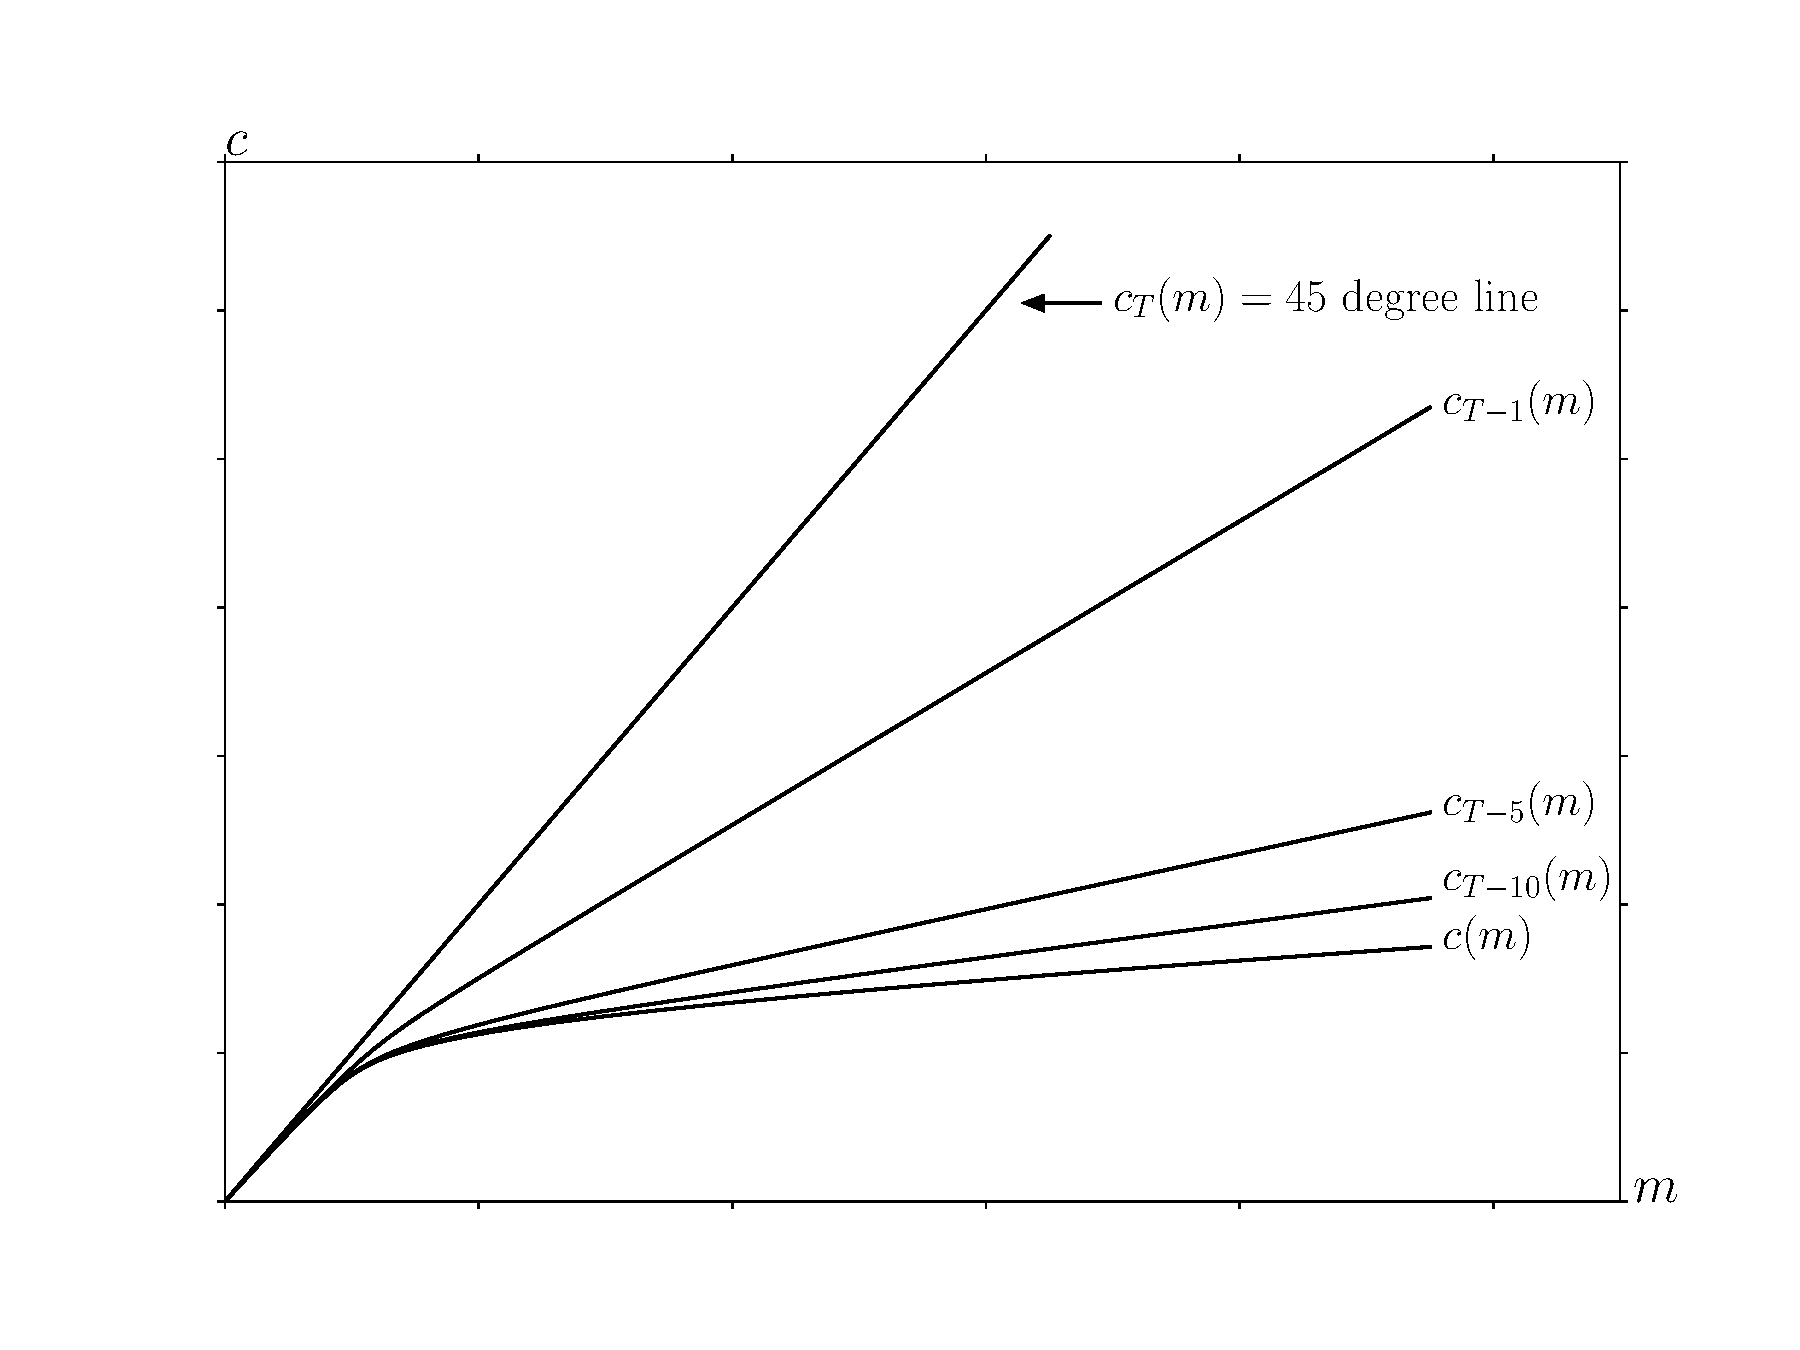
\includegraphics[width=5.25in]{\FigDir/cFuncsConverge}}
\caption{Convergence of the Consumption Rules}
\label{fig:cFuncsConverge}
\end{figure}
 % Read in the tex to generate the figure

In the figure, the consumption rules appear to converge to a nondegenerate $\usual{\cFunc}(\mRat)$.
Our next purpose is to show that this appearance is not deceptive.  \hypertarget{Concave-Consumption-Function-Characteristics}{}

\subsection{Concave Consumption Function Characteristics}\label{sec:cExists}

A precondition for the main proof is that the maximization problem defines a sequence of continuously differentiable strictly increasing strictly concave\footnote{With one obvious exception: $\usual{\cFunc}_{T}(\mRat)$ is linear (and so only weakly concave).} functions $\{\cFunc_{T},\cFunc_{T-1},\ldots\}$.  The straightforward but tedious proof is relegated to Appendix~\ref{sec:ApndxcExists}.  For present purposes, the most important point is that the income process induces what~\cite{aiyagari:ge} dubbed a `natural borrowing constraint':  $\usual{\cFunc}_{t}(\mRat) < m$ for all periods $t < T$ because a consumer who spent all available resources would arrive in period $t+1$ with balances $b_{t+1}$ of zero, and then might earn zero income over the remaining horizon, risking the possibility of a requirement to spend zero,risking negative infinite utility.  To avoid this disaster, the consumer never spends everything.~~\cite{zeldesStochastic} seems to have been the first to argue, based on his numerical results, that the natural borrowing constraint was a quantitatively plausible alternative to `artificial' or `ad hoc' borrowing constraints.\footnote{The same (numerical) point applies for infinite horizon models (calibrated to actual empirical data on household income dynamics); cf.~\cite{carrollBrookings}.}

Strict concavity and continuous differentiability of the consumption function are key elements in many of the arguments below, but are not characteristics of models with `artificial' borrowing constraints -- and we will see below that the analytical convenience of these features is considerable.% --- a point that may appeal to theorists when they realize (cf.\ Section~\ref{sec:LiqConstrAsLimit} below) that the solution to this congenial problem is arbitraily close to the solution to the constrained but less wieldy problem with explicit constraints.

\hypertarget{Bounds-for-the-Consumption-Functions}{}
\subsection{Bounds for the Consumption Functions}\label{subsec:cFuncBounds}

The consumption functions depicted in Figure~\ref{fig:cFuncsConverge} appear to have limiting slopes as $\mRat \downarrow 0$ and as $\mRat \uparrow \infty$.  This section confirms that impression and derives those slopes, which will be needed in the contraction mapping proof.\footnote{\cite{benhabibWealth} show that the consumption function becomes linear as wealth approaches infinity in a model with capital income risk and liquidity constraints;~\cite{maTodaRich} show that these results generalize to the limits derived here if capital income is added to the model.}

\newcommand{\NewMaxMinMPC}{\ushort{\MPC}}

Assume (as justified above) that a continuously differentiable concave consumption function exists in period $t+1$, with an origin at $\usual{\cFunc}_{t+1}(0)=0$, a minimal MPC $\NewMaxMinMPC_{t+1}>0$, and maximal MPC $\MaxMPC_{t+1} \leq 1$.  (If $t+1 = T$ these will be $\NewMaxMinMPC_{T}=\MaxMPC_{T}=1$; for earlier periods they will exist by recursion.)

Under our imposed assumption that human wealth is finite, the MPC bound as wealth approaches infinity is easy to understand:  As the \textit{proportion} of consumption that will be financed out of human wealth approaches zero, the proportional difference between the solution to the model with uncertainty and the perfect foresight model shrinks to zero.  \hypertarget{MPCnvrsLower}{} In the course of proving this, Appendix~\ref{sec:MPCLimits} provides a useful recursive expression (used below) for the (inverse of the) limiting MPC:\hypertarget{WRICCond}{}
\begin{align}
  \MinMPC_{t}^{-1}  & = 1+\MaxMPS \MinMPC_{t+1}^{-1} \label{eq:MinMPCInv}.
\end{align}
\subsubsection{Weak RIC Conditions}{}\label{sec:WRIC}
\hypertarget{MPCnvrsUpper}{}
\hypertarget{WRIC}{}
Equation~\eqref{eq:MaxMPCInvApndx} presents a parallel expression for the limiting maximal MPC as $\mRat_{t} \downarrow 0$:
\begin{align}\hypertarget{WRPF}{}
  \MaxMPC_{t}^{-1}  & = 1+\MinMPS \MaxMPC_{t+1}^{-1} \label{eq:MaxMPCInv}
\end{align}
where $\left\{\MaxMPC_{T-n}^{-1}\right\} _{n=0}^{\infty}$ is a decreasing % Correction per MNW 2016-01-30
convergent sequence if the `weak return patience factor' $\pZero^{1/\CRRA}\PatR$ satisfies:
\begin{align}
  0 \leq & \pZero^{1/\CRRA} \PatR < 1 \label{eq:WRIC},
\end{align}
a condition we dub the `Weak Return Impatience Condition' (\WRIC) because with $\pZero < 1$ it will hold more easily (for a larger set of parameter values) than the \RIC~($\PatR < 1$).  The essence of the argument is that as wealth approaches zero, the overriding consideration that limits consumption is the (recursive) fear of the zero-income events.  (That is why the probability of the zero income event $\pZero$ appears in the expression.)

\hypertarget{cBounds}{}
We are now in position to observe that the optimal consumption function must satisfy
\begin{align}
  \MinMinMPC_{t} \mRat_{t} ~ \leq & ~  \usual{\cFunc}_{t}(\mRat_{t})  \leq  ~ \MaxMPC_{t} \mRat_{t} \label{eq:cBounds}
\end{align}
because consumption starts at zero and is continuously differentiable, is strictly concave,\footnote{\cite{ckConcavity}} and always exhibits a slope between $\MinMinMPC_{t}$ and $\MaxMPC_{t}$ (the formal proof is in Appendix~\ref{sec:Tcomplete}).


\begin{comment}
  If the \FHWC~does not hold, we make do with a less useful bound on the minimal MPC: It is weakly greater than zero, which follows from the logic in
 ~\ref{sec:cExists}; hence the `max' in~\eqref{eq:MinMinMPCDef}.
\end{comment}

\hypertarget{Conditions-Under-Which-the-Problem-Defines-a-Contraction-Mapping}{}
\subsection{Conditions Under Which the Problem Defines a Contraction Mapping}\label{subsec:contraction}

%We can now articulate conditions under which the problem defines a contraction mapping.
As mentioned above, standard theorems in the contraction mapping literature following Stokey et.\ al.~\citeyearpar{slpMethods} require utility or marginal utility to be bounded over the space of possible values of $\mRat$, which does not hold here because the possibility (however unlikely) of an unbroken string of zero-income events through the end of the horizon means that utility (and marginal utility) are unbounded as $\mRat \downarrow 0$.  Although a recent literature examines the existence and uniqueness of solutions to Bellman equations in the presence of `unbounded returns' (see, e.g.,~\cite{mnUnique}), the techniques in that literature cannot be used to solve the problem here because the required conditions are violated by a problem that incorporates permanent shocks.\footnote{See~\cite{yaoNote} for a detailed discussion of the reasons the existing literature up through~\cite{mnUnique} cannot handle the problem described here.}

Fortunately, Boyd~\citeyearpar{jboydWeighted} provided a weighted contraction mapping theorem that~\cite{asHomogeneous} showed could be used to address the homogeneous case (of which CRRA is an example) in a deterministic framework; later,~\cite{duranDiscounting} showed how to extend the~\cite{jboydWeighted} approach to the stochastic case.
\begin{defn}
  Consider any function $\bullet\in \mathcal{C}(\mathscr{A},\mathscr{B})$ where $\mathcal{C}(\mathscr{A},\mathscr{B})$ is the space of continuous functions from $\mathscr{A}$ to $%
  \mathscr{B}$. Suppose $\phiFunc \in \mathcal{C}(\mathscr{A},\mathscr{B})$ with $%
  \mathscr{B}\subseteq\mathbb{R}$ and $\phiFunc >0$. Then $\bullet$ is $\phiFunc$-bounded if the $\phiFunc$-norm of $\bullet$,
  \begin{equation}
    \Vert \bullet\Vert _{\phiFunc }=\sup_{\mRat}\left[ \frac{|\bullet(\mRat)|}{\phiFunc (\mRat)}\right] ,
    \label{eq:phinorm}
  \end{equation}%
  is finite.
\end{defn}

For $\mathcal{C}_{\phiFunc }\left( \mathscr{A},\mathscr{B}\right) $ defined as the set of functions in $\mathcal{C}(\mathscr{A},\mathscr{B})$ that are $\phiFunc$-bounded; $\wFunc$, $\xFunc$, $\yFunc$, and $\zFunc$ as examples of $\phiFunc$-bounded functions; and using {$\mathbf{0}(\mRat)=0$} to indicate the function that returns zero for any argument, Boyd~\citeyearpar{jboydWeighted} proves the following.

\textbf{Boyd's Weighted Contraction Mapping Theorem.} \textit{Let $\BoydT:\mathcal{C}_{\phiFunc }\left( \mathscr{A},\mathscr{B}\right)
  \rightarrow \mathcal{C}\left( \mathscr{A},\mathscr{B}\right) $ such
  that}\footnote{We will usually denote the function that results from the mapping as, e.g., $\{\BoydT\wFunc\}$.}\textsuperscript{,}\footnote{To non-theorists, this notation may be slightly confusing; the inequality relations in (1) and (3) are taken to mean `for any specific element $\bullet$ in the domain of the functions in question' so that, e.g., $\xFunc \leq \yFunc$ is short for $\xFunc(\bullet) \leq \yFunc(\bullet)~\forall~\bullet\in \mathscr{A}$.  In this notation, $\zeta \Shrinker \phiFunc$ in (3) is a \textit{function} which can be applied to any argument $\bullet$ (because $\phiFunc$ is a function).} \nopagebreak
\begin{align*}
  \mbox{(1)} &\BoydT%
               \mbox{ \textit{is non-decreasing, i.e.\ ${\xFunc} \leq {\yFunc}\Rightarrow
               \{\BoydT{\xFunc}\} \leq \{\BoydT{\yFunc}\}$}}   \nonumber \\
  \mbox{(2)} & \{\BoydT\mathbf{0}\}\in ~ \mathcal{C}_{\phiFunc }\left(\mathscr{A},\mathscr{B}\right)  \notag \\
  \mbox{(3)}
             & \mbox{\textit{There exists some real $0 < \Shrinker < 1$ such that}} \\
             & \{\BoydT({\wFunc} +\zeta\phiFunc )\} \leq \{\BoydT{\wFunc}\} +\zeta\Shrinker \phiFunc
               \mbox{ \textit{~~holds for all real $\zeta > 0$ } } .
\end{align*}
\textit{Then $\BoydT$ defines a contraction with a unique fixed point.}

For our problem, take $\mathscr{A}$ as $\mathbb{R}_{>0}$ and $\mathscr{B}$
as $\mathbb{R}$, and define
\begin{align*}
  \{\EEndMap \zFunc\}(a_{t})  & = \Ex_{t}\left[\PGro^{1-\CRRA}_{t+1} \zFunc(a_{t} \Rnorm_{t+1} + \tShkAll_{t+1})\right].
\end{align*}

Using this, we introduce the mapping \textit{$\TMap:\mathcal{C}_{\phiFunc }\left( \mathscr{A},\mathscr{B}\right) \rightarrow \mathcal{C}\left( \mathscr{A},\mathscr{B}\right) $},\footnote{Note that the existence of the maximum is assured by the continuity of $\{\EEndMap \zFunc\}(a_{t})$ (it is continuous because it is the sum of continuous $\phiFunc$-bounded functions $\zFunc$) and the compactness of $[\MinMinMPC \mRat_{t}, \MaxMPC \mRat_{t}]$.}

\hypertarget{Contraction-Conditions}{}

We can show that our operator $\TMap$ satisfies the conditions that Boyd requires of his operator $\BoydT$, if we impose two restrictions on parameter values.  The first is the \WRIC~necessary for convergence of the maximal MPC, equation~\eqref{eq:WRIC} above.  More serious is the Finite Value of Autarky condition, equation~\eqref{eq:FVAC}.  (We discuss the interpretation of these restrictions in detail in Section~\ref{sec:discussConvergence} below.)  Imposing these restrictions, we are now in position to state the central theorem of the paper.

\hypertarget{MainTheorem}{}
\setcounter{theorem}{0}
\begin{theorem}\label{thm:contmap}
  $\TMap$ is a contraction mapping if the restrictions on parameter values~\eqref{eq:WRIC} and~\eqref{eq:FVAC} are true (that is, if the weak return impatience condition and the finite value of autarky condition hold).
\end{theorem}

Intuitively, Boyd's theorem shows that if you can find a $\phiFunc$ that is everywhere finite but goes to infinity `as fast or faster' than the function you are normalizing with $\phiFunc$, the normalized problem defines a contraction mapping.  The intuition for the {\FVAC} condition is that, with an infinite horizon, with any initial amount of bank balances $\bRat_{0}$, in the limit your value can always be made greater than you would get by consuming exactly the sustainable amount (say, by consuming $(\rfree/\Rfree)\bRat_{0}-\epsilon$ for some small $\epsilon>0$).

The cumbersome details of the proof are relegated to Appendix~\ref{sec:Tcomplete}.  Given that the value function converges, Appendix~\ref{subsec:cConverges} shows that the consumption functions converge.\footnote{MST's proof is for convergence of the consumption policy function directly, rather than of the value function, which is why their conditions are on $\uFunc^{\prime}$, which governs behavior.}

\hypertarget{The-Liquidity-Constrained-Solution-as-a-Limit}{}
\subsection{The Liquidity Constrained Solution as a Limit}\label{sec:deatonIsLimit}

This section explains why a related problem commonly considered in the literature (e.g., by Deaton~\citeyearpar{deatonLiqConstr}), with a liquidity constraint and a positive minimum value of income, is the limit of the problem considered here as the probability $\pZero$ of the zero-income event approaches zero.

The `related' problem makes two changes to the problem defined above:
\begin{enumerate}
\item An `artificial' liquidity constraint is imposed: $\aRat_{t}\geq 0$
  \item The probability of zero-income events is zero: $\pZero=0$
\end{enumerate}

The essence of the argument is simple.  Imposing the artificial constraint without changing $\pZero$ would not change behavior at all: The possibility of earning zero income over the remaining horizon already prevents the consumer from ending the period with zero assets.  So, for precautionary reasons, the consumer will save something.

But the \textit{extent} to which the consumer feels the need to make this precautionary provision depends on the \textit{probability} that it will turn out to matter.  As $\pZero \downarrow 0$, that probability becomes arbitrarily small, so the \textit{amount} of precautionary saving induced by the zero-income events approaches zero as $\pZero \downarrow 0$.  But ``zero'' is the amount of precautionary saving that would be induced by a zero-probability event for the impatient liquidity constrained consumer.

Another way to understand this is just to think of the liquidity
constraint reflecting a component of the utility
function that is zero whenever the consumer ends the period with
(strictly) positive assets, but negative infinity if the consumer
ends the period with (weakly) negative assets.

See Appendix~\ref{sec:LiqConstrAsLimit} for the formal proof justifying the
foregoing intuitive discussion.\footnote{It seems likely that a similar argument
  would apply even in the context of a model like that of MST, perhaps with some weak
  restrictions on returns.}

The conditions required for convergence and nondegeneracy are thus strikingly similar between the liquidity constrained perfect foresight model and the model with uncertainty but no explicit constraints: The liquidity constrained perfect foresight model is just the limiting case of the model with uncertainty as the degree of all three kinds of uncertainty (zero-income events, other transitory shocks, and permanent shocks) approaches zero.

% \hypertarget{Restrained-Consumer}{}
% In the remainder of the paper, in order to avoid a confusion that is common in discussions of models of this type, we will refer to consumers who are solving a problem in which constraints exist, but are not necessarily binding at the moment under consideration, as `restrained' consumers.

\hypertarget{Discussion-of-Parametric-Restrictions}{}
\subsection{Discussion of Parametric Restrictions}\label{sec:discussConvergence}

The full relationship among conditions is represented in Figure~\ref{fig:Inequalities}.  Though the diagram looks complex, it is merely a modified version of the earlier diagram (Figure~\ref{fig:RelatePFGICFHWCRICPFFVAC}) with further (mostly intermediate) inequalities inserted.  (Arrows with a ``because'' now label relations that always hold under the model's assumptions.)\footnote{Again, readers unfamiliar with such diagrams should see Appendix~\ref{sec:ApndxConditionDiagrams} for a more detailed exposition.}

\renewcommand{\figName}{Inequalities} % Allows generic definition of hypertargets based on title of figure
\renewcommand{\figFile}{\figName} %  and on filename
\hypertarget{\figFile}{}
%\hypertarget{\figName}{}
\input{\FigDir/\figName} % Read in the tex to generate the figure

\subsubsection{The \WRIC}\label{subsubsec:WRICdiscuss}

The `weakness' of the additional condition sufficient for contraction beyond the {\FVAC}, the
\WRIC, can be seen by asking `under what circumstances
would the \FVAC~hold but the \WRIC~fail?'
Algebraically, the requirement is
\begin{align}
  \DiscFac \PGro^{1-\CRRA}\uInvEpShkuInv^{1-\CRRA} & < ~ 1 ~ <  {(\pZero \DiscFac)}^{1/\CRRA}/\Rfree^{1-1/\CRRA}. \label{eq:WRICandFVAC}
\end{align}

If we require $\Rfree \geq 1$, the {\WRIC}~is redundant because now $\DiscFac <1<\Rfree^{\CRRA-1}$, so that (with $\CRRA > 1$ and $\DiscFac<1$) the \RIC~(and \WRIC) must hold.  But neither theory nor evidence demand that $\Rfree \geq
1$.  We can therefore approach the question of the \WRIC's relevance by asking just how low $\Rfree$ must be for the condition to be relevant.
Suppose for illustration that $\CRRA=2$, $\uInvEpShkuInv^{1-\CRRA}=1.01$,
$\PGro^{1-\CRRA}=1.01^{-1}$ and $\pZero = 0.10$.  In that case~\eqref{eq:WRICandFVAC} reduces to
\begin{align*}
  \DiscFac  & < 1 < {(0.1 \DiscFac/\Rfree)}^{1/2}
\end{align*}
but since $\DiscFac < 1$ by assumption, the binding requirement is that
\begin{align*}
  \Rfree  & < \DiscFac/10 \notag
\end{align*}
so that for example if $\DiscFac=0.96$ we would need $\Rfree < 0.096$
(that is, a perpetual riskfree rate of return of worse than -90
percent a year) in order for the \WRIC~to bind. %The relevance of the \WRIC~is indeed ``Weak.''

Perhaps the best way of thinking about this is to note that the space of parameter values for which the \WRIC~is relevant shrinks out of existence as $\pZero \rightarrow 0$, which Section~\ref{sec:deatonIsLimit} showed was the precise limiting condition under which behavior becomes arbitrarily close to the liquidity constrained solution (in the absence of other risks).  On the other hand, when $\pZero = 1$, the consumer has no noncapital income (so that the \FHWC~holds) and with $\pZero=1$ the \WRIC~is identical to the RIC;\@ but the \RIC~is the only condition required for a solution to exist for a perfect foresight consumer with no noncapital income.  Thus the WRIC~forms a sort of `bridge' between the liquidity constrained and the unconstrained problems as $\pZero$ moves from 0 to 1.

\hypertarget{IntuitionRIC}{}
\subsubsection{When the \RIC~Fails}\label{subsubsec:WhenTheRICFails}

In the perfect foresight problem (Section~\ref{subsec:PFUncon}), the \RIC~was necessary for existence of a nondegenerate solution.  It is surprising, therefore, that in the presence of uncertainty, the much weaker {\WRIC} is sufficient for nondegeneracy (assuming that the {\FVAC} holds).
\begin{comment}
  But if the \RIC~does hold, some useful results can be derived.  Arguably
  the most fundamental are that the limiting values
  for the minimal and maximal marginal propensities to consume implicit in
 ~\eqref{eq:MaxMPCInv} and~\eqref{eq:MinMPCInv} are positive and finite.
\end{comment}
We can directly derive the features the problem must
exhibit (given the \FVAC) under \cncl{\RIC} (that is, $\Rfree < {(\Rfree \DiscFac)}^{1/\CRRA})$:
\begin{align}
  \Rfree   & < \overbrace{{(\Rfree \DiscFac)}^{1/\CRRA} ~ < ~ {(\Rfree {(\PGro \uInvEpShkuInv)}^{\CRRA-1})}^{1/\CRRA}}^{\text{implied by \FVAC}} \notag
  \\  \Rfree   & < {(\Rfree/\PGro)}^{1/\CRRA}\PGro \uInvEpShkuInv^{1-1/\CRRA} \notag
  \\  \Rfree/\PGro  & < {(\Rfree/\PGro)}^{1/\CRRA}\uInvEpShkuInv^{1-1/\CRRA} \notag
  \\  \Rfree/\PGro  & < \uInvEpShkuInv \label{eq:RICimplies}
\end{align}
but since $\uInvEpShkuInv < 1$ (cf.\ the argument below~\eqref{eq:uInvEpShkuInv}), this requires $\Rfree/\PGro < 1$; so, given the \FVAC, the \RIC~can fail only if human wealth is unbounded.  As an illustration of the usefulness of our diagrams, note that this algebraically complicated conclusion could be easily reached diagrammatically in figure~\ref{fig:Inequalities} by starting at the $\Rfree$ node and imposing $\cncl{\RIC}$, reversing the {\RIC} arrow and then traversing the diagram along any clockwise path to the {\PFVAF} node at which point we realize that we \textit{cannot} impose the {\FHWC} because that would let us conclude $\Rfree > \Rfree$.

As in the perfect foresight constrained problem, unbounded limiting human wealth (\cncl{\FHWC}) here does not lead to a degenerate limiting consumption function (finite human wealth is not a condition required for the convergence theorem).  But, from equation~\eqref{eq:MinMPCInv} and the discussion surrounding it, an implication of \cncl{\RIC} is that $\lim_{m \uparrow \infty} \usual{\cFunc}^{\prime}(\mRat) = 0$.  Thus, interestingly, in the special $\{\cncl{\RIC},\cncl{\FHWC}\}$ case (unavailable in the perfect foresight model) the presence of uncertainty both permits unlimited human wealth (in the $n\uparrow\infty$ limit) and at the same time prevents unlimited human wealth from resulting in (limiting) infinite consumption at any finite $\mRat$.  Intutively, in the presence of uncertainty, pathological patience (which in the perfect foresight model results in a limiting consumption function of $\usual{\cFunc}(\mRat)=0$ for finite $\mRat$) plus unbounded human wealth (which the perfect foresight model prohibits because it leads to a limiting consumption function $\usual{\cFunc}(\mRat)=\infty$ for any finite $\mRat$) combine to yield a unique finite level of consumption and MPC for any finite value of $\mRat$.  Note the close parallel to the conclusion in the perfect foresight liquidity constrained model in the \{\GICRaw,\cncl{\RIC}\} case.  There, too, the tension between infinite human wealth and pathological patience was resolved with a nondegenerate consumption function whose limiting MPC was zero.\footnote{\cite{maTodaRich} derive conditions under which the limiting MPC is zero in an even more general case where there is also capital income risk.}

\hypertarget{When-the-RIC-Holds}{}
\subsubsection{When the {\RIC} Holds}\label{subsubsec:WhenTheGICNrmFails}\label{subsubsec:WhenTheRICHolds}

\indent \textbf{\FHWC}.  If the {\RIC} and {\FHWC} both hold, a perfect foresight solution exists (see~\ref{subsec:PFUncon} above).  As $\mRat \uparrow \infty$ the limiting consumption function and value function become arbitrarily close to those in the perfect foresight model, because human wealth pays for a vanishingly small portion of spending.  This will be the main case analyzed in detail below.

\begin{comment}
\begin{align}
  \Rfree^{1/\CRRA}\PGro^{1-1/\CRRA}\uInvEpShkuInv^{1-1/\CRRA} & < \Pat <   \Rfree^{1/\CRRA}\PGro^{1-1/\CRRA}
  \\   \uInvEpShkuInv^{1-1/\CRRA}(\Rfree/\PGro)^{1/\CRRA-1} & < \PatR < 1 < (\Rfree/\PGro)^{1/\CRRA-1}
  \\   \uInvEpShkuInv^{1-1/\CRRA}\Rfree^{1/\CRRA-1}\PGro^{1-1/\CRRA}                                                               & < \Rfree^{1/\CRRA}\DiscFac^{1/\CRRA}/\Rfree < 1 < \Rfree^{1/\CRRA-1}\PGro^{1-1/\CRRA}
  \\   \uInvEpShkuInv^{1-1/\CRRA}\Rfree^{-1}\PGro^{1-1/\CRRA}                                                               & < \DiscFac^{1/\CRRA}/\Rfree < \Rfree^{-1/\CRRA} < \Rfree^{-1}\PGro^{1-1/\CRRA}
  \\   \uInvEpShkuInv^{1-1/\CRRA}\PGro^{1-1/\CRRA}                                                               & < \DiscFac^{1/\CRRA} < \Rfree^{1-1/\CRRA} < \PGro^{1-1/\CRRA}
  \\   \uInvEpShkuInv^{(\CRRA-1)/\CRRA}\PGro^{(\CRRA-1)/\CRRA}                                                               & < \DiscFac^{1/\CRRA} < \Rfree^{(\CRRA-1)/\CRRA} < \PGro^{(\CRRA-1)/\CRRA}
  \\   \uInvEpShkuInv^{\CRRA-1} & < \DiscFac/\PGro < 1
  \\   \PGro \uInvEpShkuInv^{\CRRA-1} & < \DiscFac < \PGro
\end{align}
\end{comment}

\noindent \textbf{\cncl{\FHWC}}.  The more exotic case is where {\FHWC} does not hold; in the perfect foresight model, \{{\RIC},\cncl{\FHWC}\} is the degenerate case with limiting $\bar{\cFunc}(\mRat)=\infty$.  Here, since the {\FVAC} implies that the {\PFFVAC} holds (traverse Figure~\ref{fig:Inequalities} clockwise from $\Pat$ by imposing {\FVAC} and continue to the {\PFVAF} node):  Reversing the arrow connecting the $\Rfree$ and {\PFVAF} nodes implies that under $\cncl{\FHWC}$:
\begin{align*}
   & \overbrace{\Pat < {(\Rfree/\PGro)}^{1/\CRRA}\PGro}^{\PFFVAC}
      \\ & \Pat < \PGro
\end{align*}
where the transition from the first to the second lines is justified because $\cncl{\FHWC} \Rightarrow {(\Rfree/\PGro)}^{1/\CRRA}<1$.  So, \{\RIC, \cncl{\FHWC}\} implies the {\GICRaw} holds.  However, we are not entitled to conclude that the {\GICNrm} holds: $\Pat < \PGro$ does not imply $\Pat < \InvEpShkInv \PGro$ where $\InvEpShkInv<1$.  %See further discussion of this illuminating case in section~\ref{subsubsec:FVACnotGIC}.

\begin{comment}

Finally, we are entitled to conclude that $\lim_{\mRat \uparrow \infty} \MPC(\mRat) = \MinMPC$ because, for any fixed value of $\pZero > 0$, and any fixed horizon $n$ it must be true that:
\begin{enumerate}
\item $\usual{\cFunc}_{T-n}(\mRat) < \bar{\cFunc}_{T-n}$ for the reasons described in the section on the liquidity constrained model above
  \item As $\mRat \uparrow \infty$ the \textit{amount} by which $\bar{\cFunc}$ exceeds $\usual{\cFunc}$ approaches zero.
\end{enumerate}

%This result introduces the discussion of the last interesting parametric question, which is implications the alternative versions of the Growth Impatience Condition (continuing to assume the {\FVAC} and {\WRIC} conditions required for nondegeneracy).
\end{comment}

We have now established the principal points of comparison between the perfect foresight solutions and the solutions under uncertainty; these are codified in the remaining parts of Tables~\ref{table:Comparison} and~\ref{table:Required}.

\hypertarget{Factors-Defined-And-Compared}{}
  \let\TableWidth\relax
  \newlength\TableWidth
  \newsavebox{\ComparisonSub}
  \begin{table}[!th]
    \centering
\caption{Definitions and Comparisons of Conditions}\label{table:Comparison}
  \sbox{\ComparisonSub}{
\begin{tabular}{|c|c|}\hline
Perfect Foresight Versions & Uncertainty Versions\\ \hline
\multicolumn{2}{|c|}{Finite Human Wealth Condition (\FHWC)} \\ \hline
$\PGro/\Rfree < 1$                                                          & $\PGro/\Rfree < 1$ \\
\multirow{3}{75mm}{\thead{The growth factor for permanent income \\ $\PGro$ must be smaller than the discounting \\ factor $\Rfree$ for human wealth to be finite. }} &
\multirow{3}{75mm}{\thead{The model's risks are mean-preserving \\ spreads, so the PDV of future income is \\ unchanged by their introduction.}} \\
&  \\
&  \\
&  \\ \hline
\multicolumn{2}{|c|}{Absolute Impatience Condition (\AIC)} \\ \hline
$\Pat < 1$                                        &  $\Pat < 1$ \\
\multirow{4}{75mm}{\thead{The unconstrained consumer is \\ sufficiently impatient that the level of \\ consumption will be declining over time:}} &
\multirow{4}{75mm}{\thead{\textit{If wealth is large enough,} the \textit{expectation} \\ of consumption next period will be \\ smaller than this period's consumption:}} \\
& \\
& \\
& \\
$\cLevBF_{t+1} < \cLevBF_{t}$ & $\lim_{m_{t} \rightarrow \infty} \Ex_{t} [\cLevBF_{t+1}] < \cLevBF_{t}$ \\
& \\ \hline
\multicolumn{2}{|c|}{Return Impatience Conditions} \\ \hline
\multicolumn{1}{|c|}{Return Impatience Condition (\RIC)} & \multicolumn{1}{c|}{Weak \RIC~(\WRIC)} \\ \hline
$\Pat/\Rfree < 1$                                          & $\pZero^{1/\CRRA}\Pat/\Rfree < 1$ \\
\multirow{3}{75mm}{\thead{The growth factor for consumption $\Pat$ \\ must be smaller than the discounting \\ factor $\Rfree$, so that the PDV of current and \\ future consumption will be finite:}}  &
\multirow{3}{75mm}{\thead{If the probability of the zero-income \\ event is $\pZero=1$ then income is always zero \\ and the condition becomes identical to \\ the \RIC.  Otherwise, weaker.}} \\
& \\
& \\
& \\
& \\
$\cFunc^{\prime}(m) = 1-\Pat/\Rfree < 1$              & $\cFunc^{\prime}(m) < 1-\pZero^{1/\CRRA}\Pat/\Rfree < 1$ \\
& \\ \hline
\multicolumn{2}{|c|}{Growth Impatience Conditions} \\ \hline
\multicolumn{1}{|c|}{\GICRaw} & \multicolumn{1}{c|}{\GICNrm} \\ \hline
$\Pat/\PGro < 1$                                         & $\Pat\Ex[\pShk^{-1}]/\PGro < 1 $ \\
\multirow{4}{75mm}{\thead{For an unconstrained PF consumer, the \\ ratio of $\cLevBF$ to $\pLevBF$ will fall over time.  For \\ constrained, guarantees the constraint \\ eventually binds. Guarantees \\ ~~~~~~$\lim_{\mRat_{t}\uparrow\infty} \Ex_{t}[\pShk_{t+1}\mRat_{t+1}/\mRat_{t}] = \PatPGro$}} &
\multirow{4}{75mm}{\thead{By Jensen's inequality stronger than \GICRaw.\\  Ensures consumers will not expect to \\ accumulate $\mRat$ unboundedly.}} \\
& \\
& \\
& \\
& $\lim_{\mRat_{t} \rightarrow \infty} \Ex_{t}[\mRat_{t+1}/\mRat_{t}] = \PatPGroAdj $
 \\
&  \\ \hline
\multicolumn{2}{|c|}{Finite Value of Autarky Conditions} \\ \hline
\multicolumn{1}{|c|}{\PFFVAC} & \multicolumn{1}{c|}{\FVAC} \\ \hline
$\beta \PGro^{1-\CRRA} < 1$                                                 & $\beta \PGro^{1-\CRRA}\Ex[\pshk^{1-\CRRA}] < 1$  \\
equivalently $\Pat  < \Rfree^{1/\CRRA}\PGro^{1-1/\CRRA}$ & \\
\multirow{3}{75mm}{\thead{The discounted utility of constrained \\ consumers who spend their permanent \\ income each period should be finite.}} &
\multirow{3}{75mm}{\thead{By Jensen's inequality, stronger than the \\ \PFFVAC~because for $\CRRA>1$ and \\ nondegenerate $\pShk$, $\Ex[\pShk^{1-\CRRA}] > 1$.} } \\
& \\
                           & \\
&  \\ \hline
\end{tabular}
} % End \sbox
\settowidth\TableWidth{\usebox{\ComparisonSub}}
\usebox{\ComparisonSub}
\end{table}


\hypertarget{Sufficient-Conditions}{}
\hypertarget{Sufficient-Conditions-For-Nondegenerate-Solution}{}

\newsavebox{\Required}
\begin{table}
\centering
\caption{Conditions for Nondegenerate$^{\ddagger}$ Solution} \label{table:Required}
\sbox{\Required}{
\begin{tabular}{|l|l|l|} \hline
  \multicolumn{1}{|l|}{Consumption Model(s)}                                                                             & \multicolumn{1}{c|}{Conditions}         & \multicolumn{1}{c|}{Comments}
%    \\\multicolumn{1}{|r|}{ Reference            }                                                                         &                                         & \multicolumn{1}{c|}{Logic}
    \\ \hline
        \multicolumn{1}{|l|}{$\bar{\cFunc}(m)$: PF Unconstrained}                                                              & \RIC, \FHWC$^{\circ}$                   & \RIC$\Rightarrow |\vFunc(\mRat)|< \infty$; \FHWC$ \Rightarrow 0 < |\vFunc(\mRat)|$
    \\ {$\underline{\cFunc}(m)=\MinMPC \mRat$}                                                                &                                         & PF model with no human wealth ($h=0$)
    \\\multicolumn{1}{|l|}{}                                                                         &                                          \multicolumn{1}{c|}{} &                                          \multicolumn{1}{c|}{}
    \\ \multicolumn{1}{|r|}{\href{https://\owner.github.io/BufferStockTheory\#PF-Unconstrained-Solution}{Section \ref{subsec:PFUncon}:}}         &                                         & \RIC prevents $\bar{\cFunc}(\mRat)=\underline{\cFunc}(\mRat)=0$
    \\ \multicolumn{1}{|r|}{\href{https://\owner.github.io/BufferStockTheory\#PF-Unconstrained-Solution}{Section \ref{subsec:PFUncon}:}}         &                                         & \FHWC prevents $\bar{\cFunc}(\mRat)=\infty$
    \\ \multicolumn{1}{|r|}{Eq \eqref{eq:FHWCandPFFVACimplyRIC}:}                                                                              &                                         & {\PFFVAC}+{\FHWC} $\Rightarrow$ {\RIC}
    \\ \multicolumn{1}{|r|}{{Eq \eqref{eq:GICandFHWCimplyPFFVAC}}:}                                                                              &                                         & {\GIC}+{\FHWC} $\Rightarrow$ {\PFFVAC}
    \\ \hline\hline \multicolumn{1}{|l|}{$\constr{\cFunc}(m)$: PF Constrained}                                              & \cncl{\GICRaw}, \RIC                    & {\FHWC} holds $(\PGro < \Pat < \Rfree \Rightarrow \PGro < \Rfree)$
    \\
\multicolumn{1}{|r|}{\href{https://\owner.github.io/BufferStockTheory\#PF-Constrained-Solution}{Section \ref{subsec:PFCon}:}}                &                                         & $\constr{\cFunc}(\mRat)=\bar{\cFunc}(\mRat)$ for $\mRat > \mRat_{\#} < 1$
    \\                                                                                                                        &                                         & (\cncl{\RIC} would yield $\mRat_{\#}=0$ so $\constr{\cFunc}(\mRat)=0$)
%  \\ \cline{2-3} \href{https://\owner.github.io/BufferStockTheory\#ApndxLiqConstr}{Appendix \ref{sec:ApndxLiqConstr}} & \GICRaw,\RIC                            & $\lim_{\mRat \rightarrow \infty} \constr{\cRat}(\mRat)=\bar{\cRat}(\mRat), \lim_{\mRat \rightarrow \infty} \constr{\MPCFunc}(\mRat)=\MinMPC$
    \\ \cline{2-3}  \multicolumn{1}{|r|}{\href{https://\owner.github.io/BufferStockTheory\#ApndxLiqConstr}{Appendix \ref{sec:ApndxLiqConstr}}:} & \GICRaw,\RIC                            & $\lim_{\mRat \rightarrow \infty} \constr{\cRat}(\mRat)=\bar{\cRat}(\mRat), \lim_{\mRat \rightarrow \infty} \constr{\MPCFunc}(\mRat)=\MinMPC$
    \\                                                                                                                        &                                         & kinks where horizon to $b=0$ changes$^{\ast}$
    \\ \cline{2-3}\multicolumn{1}{|r|}{\href{https://\owner.github.io/BufferStockTheory\#ApndxLiqConstr}{Appendix \ref{sec:ApndxLiqConstr}}:}  & \GICRaw,\cncl{\RIC}                     & $\lim_{\mRat \rightarrow \infty}  \constr{\MPCFunc}(\mRat)=0$
    \\                                                                                                                        &                                         & kinks where horizon to $b=0$ changes$^{\ast}$
    \\ \hline\hline \multicolumn{1}{|l|}{$\usual{\cFunc}(\mRat)$:  \href{https://\owner.github.io/BufferStockTheory\#Uncertainty-Modified-Conditions}{Friedman/Muth}
  }                                                                                                                       & Section \ref{subsec:LimitsAsmtToInfty}, & $\underline{\cFunc}(\mRat) < \usual{\cFunc}(\mRat) < \bar{\cFunc}(\mRat)$ %\phantom{\RIC, \FHWC$^{\ast\ast}$  }
    \\                                                                                                                      & Section \ref{subsec:LimitsAsmtToZero}   & $\underline{\vFunc}(\mRat) < \usual{\vFunc}(\mRat) < \bar{\vFunc}(\mRat)$ %
  % \\ \hline\hline \multicolumn{1}{|l|}{$\usual{\cFunc}(\mRat)$: Friedman/Muth}                                          & \FVAC, \WRIC                            & \WRIC is weaker than \RIC 
%   \\ {``Buffer Stock'' Subset}                                                                                       &                                         & \GICNrm $\Rightarrow \exists $ `individual target' $\mTrg$
%   \\ { Section \ref{subsec:onetarget}}                                                                             &                                         & \GIC $\Rightarrow \exists $ `individual steady-state' $\mStE$

  \\ \cline{2-3}\multicolumn{1}{|r|}{Section \ref{subsec:contraction}:}                            & \FVAC, \WRIC                      & Sufficient for Contraction
 \\ \multicolumn{1}{|r|}{Section \ref{subsubsec:WRICdiscuss}:}                               &                      & \WRIC is weaker than \RIC 
\\  \multicolumn{1}{|r|}{Figure \ref{fig:Inequalities}:}                                        &                                 & \FVAC is stronger than \PFFVAC 
  \\ \multicolumn{1}{|r|}{Section \ref{subsubsec:WhenTheRICHolds}:}
                                            &                                 & \cncl{\FHWC}+RIC $\Rightarrow $\GIC$, \lim_{\mRat \rightarrow \infty} \usual{\MPCFunc}(\mRat)=\MinMPC$
  \\  \multicolumn{1}{|r|}{Section \ref{subsubsec:WhenTheRICFails}:}                                        &                                 & \cncl{\RIC}  $\Rightarrow $\cncl{\FHWC}$, \lim_{\mRat \rightarrow \infty} \usual{\MPCFunc}(\mRat)=0$
  \\ \cline{3-3}\multicolumn{1}{|r|}{Section \ref{subsec:onetarget}:}                                        &                                 & ``Buffer Stock Saving'' Conditions
  \\ \multicolumn{1}{|r|}{Section \ref{subsubsec:mSteadyState}:}                                        &                                 & \phantom{-Nrm}{\GIC} $\Rightarrow \exists 0 < \mStE < \infty$ %: Steady-State
  \\ \multicolumn{1}{|r|}{Section \ref{subsubsec:mTarget}:}                                        &                                 & {\GICNrm} $\Rightarrow \exists 0 < \mTrg < \infty$ %: Target
%  \\ \hline\hline \multicolumn{1}{|l|}{$\usual{\cFunc}(\mRat)$: Friedman/Muth} & \RIC, \FHWC                      & $\underline{\cFunc}(\mRat) < \usual{\cFunc}(\mRat) < \bar{\cFunc}(\mRat)$
%  \\ {``Buffer Stock'' Subset}                                         &                                 & \GICNrm $\Rightarrow \exists $ `individual target' $\mTrg$
%\\ { Section \ref{subsec:onetarget}}                                         &                                 & \GIC $\Rightarrow \exists $ `individual steady-state' $\mStE$

\\ \hline \multicolumn{3}{c}{}
\end{tabular}
} % End \sbox

\settowidth\TableWidth{\usebox{\Required}}
%\usebox{\Required}
\newlength{\RequiredShrunk}
\newsavebox{\RequiredShrunkBox}

\savebox{\RequiredShrunkBox}{
  \settowidth{\RequiredShrunk}{\usebox{\Required}}
  \resizebox{\textwidth}{!}{\begin{minipage}{\RequiredShrunk}
      \usebox{\Required}
    \end{minipage}}
}

\usebox{\RequiredShrunkBox}


\parbox{\textwidth}{\footnotesize         $^{\ddagger}$For feasible $\mRat$ satisfying $0 < \mRat < \infty$, a nondegenerate limiting consumption function defines a unique optimal value of $\cRat$ satisfying $0 < \cRat(m) < \infty$; a nondegenerate limiting value function defines a corresponding unique value of $-\infty < \vFunc(\mRat) < 0$ .  $^{\circ}$RIC, \FHWC are necessary as well as sufficient for the perfect foresight case.  $^{\ast}$That is, the first kink point in $\cRat(\mRat)$ is $\mRat_{\#}$ s.t. for $\mRat < \mRat_{\#}$ the constraint will bind now, while for $\mRat > \mRat_{\#}$ the constraint will bind one period in the future.  The second kink point corresponds to the $\mRat$ where the constraint will bind two periods in the future, etc.$^{\ast\ast}$In the Friedman/Muth model, the {\RIC}+{\FHWC} are sufficient, but \textit{not} necessary for nondegeneracy}
\end{table}



\hypertarget{AnalysisoftheConvergedConsumptionFunction}{}
\section{Analysis of the Converged Consumption Function}\label{sec:convergedcfunc}

Figures~\ref{fig:cGroTargetFig}-\ref{fig:cFuncBounds} capture the main properties of the converged consumption rule when the \RIC, \GICNrm, and \FHWC~all hold.\footnote{These figures reflect the converged rule corresponding to the parameter values indicated in Table~\ref{table:Calibration}.}

Figure~\ref{fig:cGroTargetFig} shows the expected growth factors for consumption, the level of market resources, and the market resources ratio, $\Ex_{t}[\cLevBF_{t+1}/\cLevBF_{t}]$ and $\Ex_{t}[\mLevBF_{t+1}/\mLevBF_{t}]$, and $\Ex_{t}[\mRat_{t+1}/\mRat_{t}]$, for a consumer behaving according to the converged consumption rule, while Figures~\ref{fig:mpclimits}---\ref{fig:cFuncBounds} illustrate theoretical bounds for the consumption function and the MPC.

Three features of behavior are captured, or suggested, by the figures.

First, as $\mRat_{t} \uparrow \infty$ the expected consumption growth factor goes to ${\Pat}$, indicated by the lower bound in Figure~\ref{fig:cGroTargetFig}, and the marginal propensity to consume approaches $\MinMPC=(1-\PatR)$ (see Figure~\ref{fig:mpclimits}) --- the same as the perfect foresight MPC.\@  Second, as $\mRat_{t}$ approaches zero the consumption growth factor approaches $\infty$ (Figure~\ref{fig:cGroTargetFig}) and the MPC approaches $\MaxMPC=(1-\pZero^{1/\CRRA}\PatR)$ (Figure~\ref{fig:mpclimits}).  Third, there is a value $\mRat = \hat{\mRat}$ at which the expected growth rate of $\mLevBF$ matches the expected growth rate of permanent income $\PGro$, and a different (lower) value where the expected growth rate of consumption at $\mRat = \hat{\mRat}$ is lower than $\PGro$.  Thus, at the individual level, this model does not have a `balanced growth' equilibrium.\footnote{A final proposition suggested by Figure~\ref{fig:cGroTargetFig} is that the expected consumption growth factor is declining in the level of the cash-on-hand ratio $\mRat_{t}$.  This turns out to be true in the absence of permanent shocks, but in extreme cases it can be false if permanent shocks are present; see Appendix~\ref{sec:ApndxCGrowthDeclines}.}

\begin{comment}
  Third (Figure~\ref{fig:cGroTargetFig}), there are two special values of $\mRat$, which we will call the `individual balanced growth' point $\mStE$ because it is the point where expected consumption growth and expected permanent income growth are balanced, and the `individual target' $\mTrg$ such that if $\mRat_t = \mTrg$ then $\Ex_t [{\mRat}_{t+1}] = \mRat_t$.  %As indicated by the arrows of motion on the $\Ex_{t}[\cLevBF_{t+1}/\cLevBF_{t}]$ curve, the model's dynamics are `stable' around this target in the sense that if $\mRat_{t} < \mTrg$ then $\mRat$ will rise (in expectation), while if $\mRat_{t} > \mTrg$, it will fall (in expectation).Fourth (Figure~\ref{fig:cGroTargetFig}), at the market resources target $\mTrg$, the expected rate of growth of consumption is slightly less than the expected growth rate
  of permanent noncapital income.  (The individual consumer does not expect `balanced growth' at $\mTrg$).

  The final proposition suggested by Figure~\ref{fig:cGroTargetFig} is that the expected consumption growth factor is declining in the level of the cash-on-hand ratio $\mRat_{t}$.  This turns out to be true in the absence of permanent shocks, but in extreme cases it can be false if permanent shocks are present.\footnote{Throughout the remaining analysis I make a final assumption that is not strictly justified by the foregoing.  We have seen that the finite-horizon consumption functions $\usual{\cFunc}_{T-n}(\mRat)$ are twice continuously differentiable and strictly concave, and that they converge to a continuous function $\usual{\cFunc}(\mRat)$.  It does not strictly follow that the limiting function $\usual{\cFunc}(\mRat)$ is twice continuously differentiable, but I will assume that it is.}
\end{comment}

\renewcommand{\figFile}{cGroTargetFig}
\hypertarget{\figFile}{}
% Could not get fonts to work right for svg version of this figure for web; so use png
\ifthenelse{\boolean{Web}}{
\begin{figure}[tbp]
\centerline{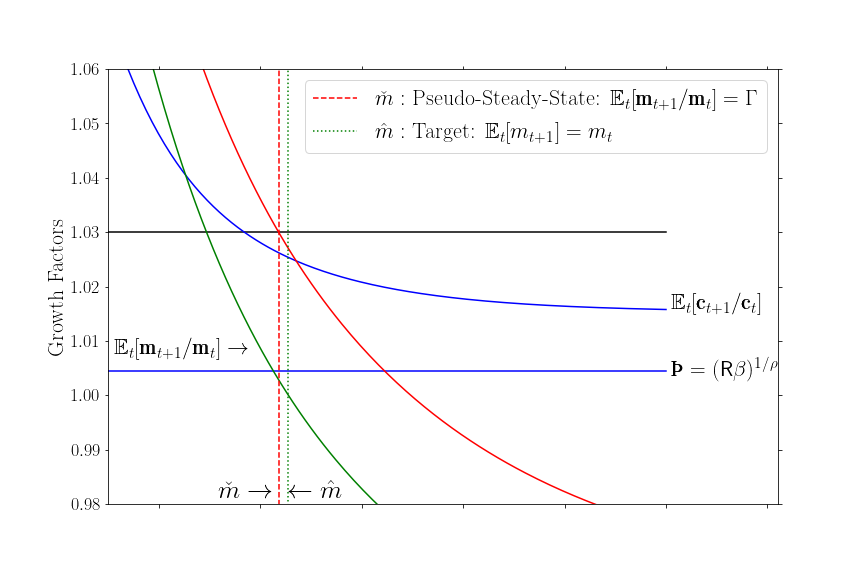
\includegraphics[width=8in]{\FigDir/cGroTargetFig.png}}
\caption{`Stable' $\mRat$ Values and Expected Growth Rates}
\label{fig:cGroTargetFig}
\end{figure}
}{
\begin{figure}[tbp]
\centerline{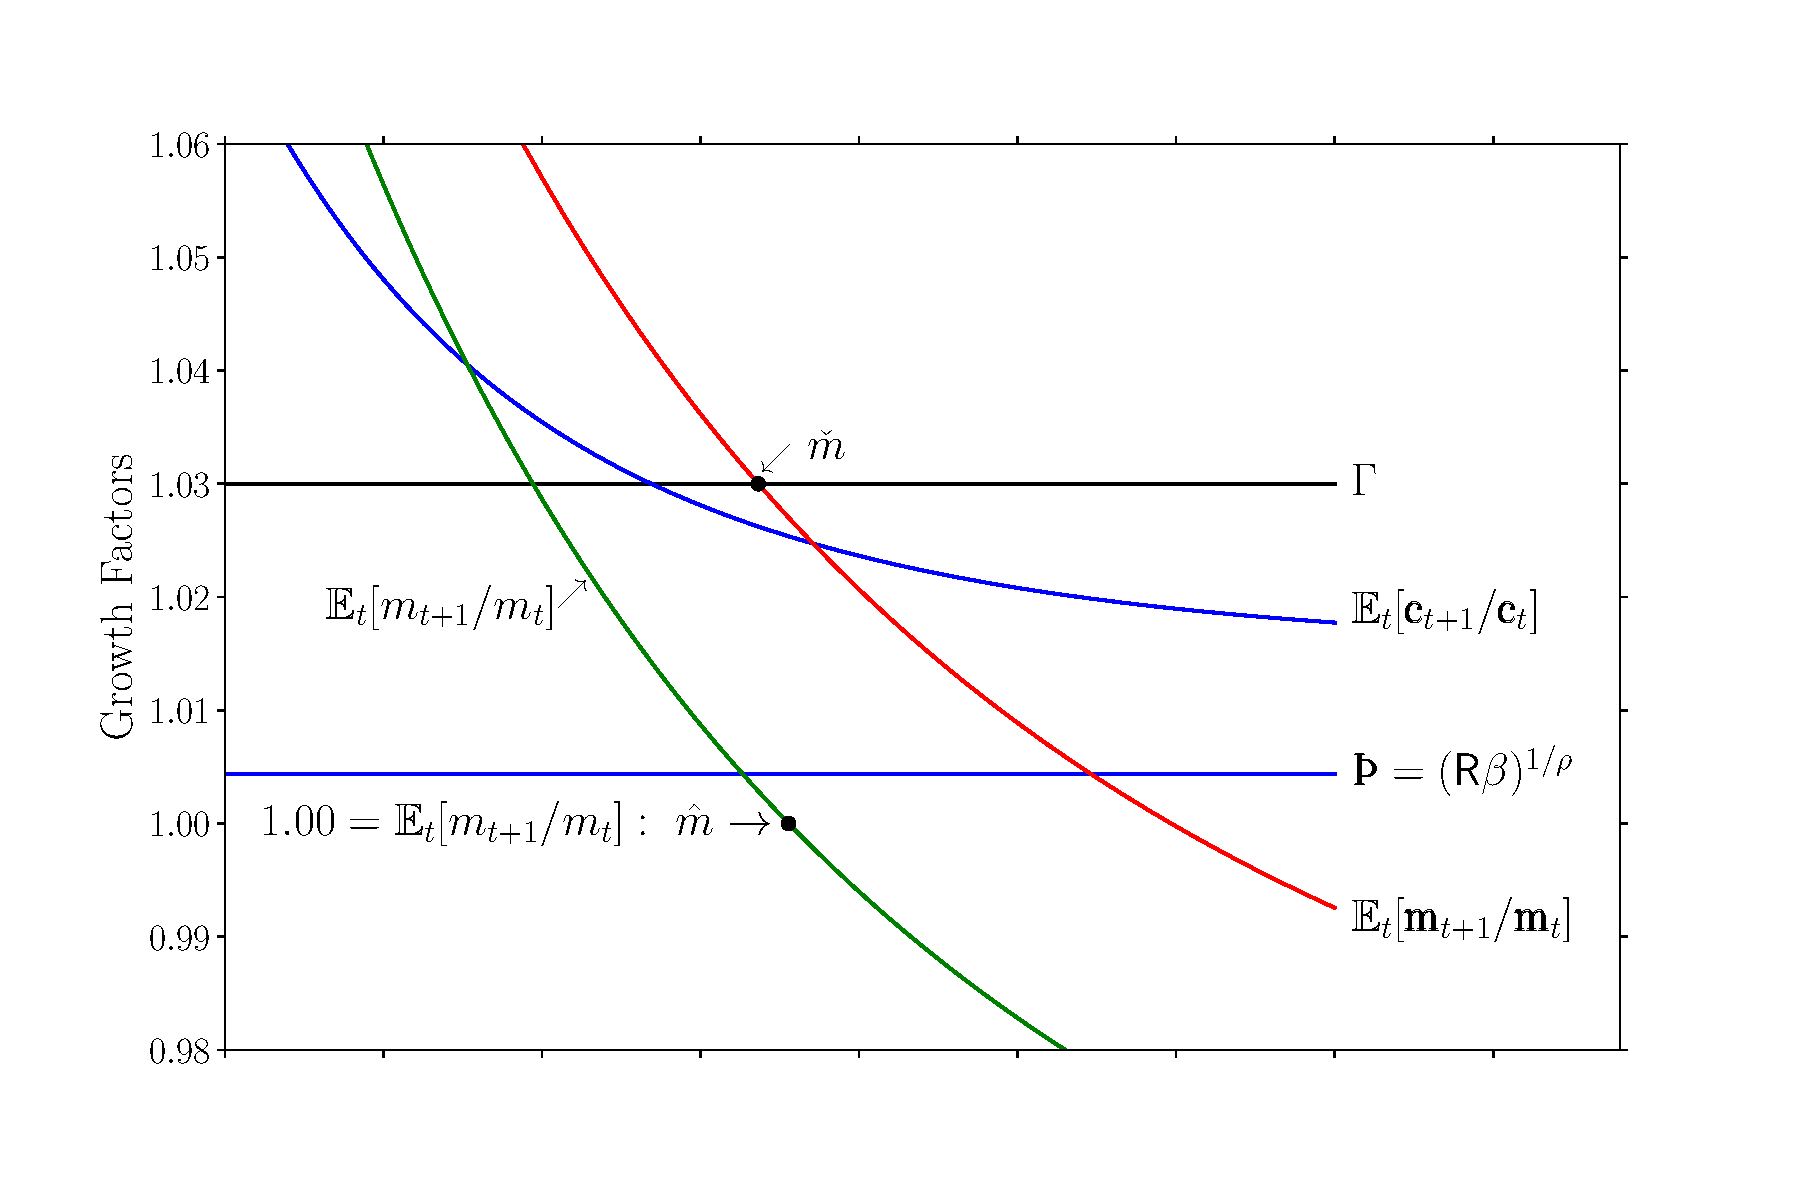
\includegraphics[width=6in]{\FigDir/cGroTargetFig}}
\caption{`Stable' $\mRat$ Values and Expected Growth Factors}
\label{fig:cGroTargetFig}
\end{figure}
}


\hypertarget{LimitsAsmtToInfty}{}
\subsection{Limits as \texorpdfstring{$\mRat$}{m} approaches Infinity}\label{subsec:LimitsAsmtToInfty}

Define
\begin{align*}
  \ushort{\cFunc}(\mRat)  & = \MinMPC \mRat
\end{align*}
which is the solution to an infinite-horizon problem with no noncapital income ($\tShkAll_{t+n} = 0~\forall~n\geq1$); clearly $\ushort{\cFunc}(\mRat) < \usual{\cFunc}(\mRat)$, since allowing the possibility of future noncapital income cannot reduce current consumption.  Our imposition of the {\RIC} guarantees that $\MinMPC > 0$, so this solution satisfies our definition of nondegeneracy, and because this solution is always available it defines a lower bound on both the consumption and value functions.%\footnote{We will assume the \RIC~holds here and subsequently so that $\MinMPC > 0$; the situation is a bit more complex when the \RIC~does not hold.  In that case the bound on consumption is given by the spending that would be undertaken by a consumer who faced binding liquidity constraints.}

Assuming the \FHWC~holds, the infinite horizon perfect foresight solution~\eqref{eq:cFuncPFUnc} constitutes an upper bound on consumption in the presence of uncertainty, since the introduction of uncertainty strictly decreases the level of consumption at any $\mRat$ (\cite{ckConcavity}).  Thus, we can write
\begin{align}
  \ushort{\cFunc}(\mRat) < & \usual{\cFunc}(\mRat)  < \bar{\cFunc}(\mRat) \label{eq:lowerltupper} \\
  1 < & \usual{\cFunc}(\mRat)/\ushort{\cFunc}(\mRat)  < \bar{\cFunc}(\mRat)/\ushort{\cFunc}(\mRat). \nonumber
\end{align}
But
\begin{align*}  \label{eq:limitlowerupper}
  \lim_{m \uparrow \infty} \bar{\cFunc}(\mRat)/\ushort{\cFunc}(\mRat)
  & = \lim_{m \uparrow \infty} (\mRat -1+ \hRat)/\mRat  \\
  & = 1,
\end{align*}
so as $\mRat \uparrow \infty, \usual{\cFunc}(\mRat)/\ushort{\cFunc}(\mRat)
\rightarrow 1$, and the continuous differentiability and strict
concavity of $\usual{\cFunc}(\mRat)$ therefore implies
\begin{equation*}  \label{eq:limxtoinftycp}
  \lim_{m \uparrow \infty} \usual{\cFunc}^{\prime}(\mRat) =
  \ushort{\cFunc}^{\prime}(\mRat) = \bar{\cFunc}^{\prime}(\mRat) = \MinMPC
\end{equation*}
because any other fixed limit would eventually lead to a level of
consumption either exceeding $\bar{\cFunc}(\mRat)$ or lower than
$\ushort{\cFunc}(\mRat)$.

Figure~\ref{fig:mpclimits} confirms these limits visually.  The top
plot shows the converged consumption function along with its upper and lower bounds,
while the lower plot shows the marginal propensity to consume.

\renewcommand{\figFile}{mpclimits}
\hypertarget{\figFile}{}
\hypertarget{MPCLimits}{}
\begin{figure}
\centerline{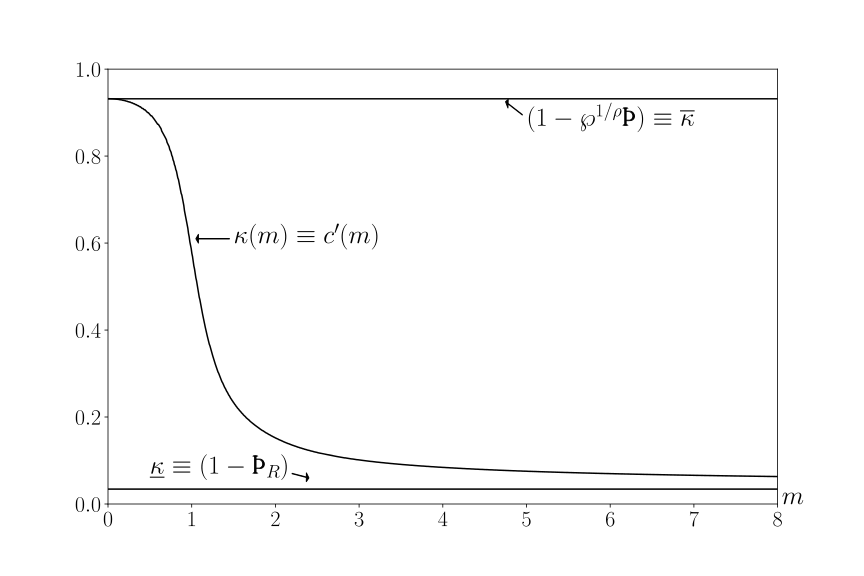
\includegraphics[width=6in]{\FigDir/MPCLimits}}
\caption{Limiting MPC's}
\label{fig:mpclimits}
\end{figure}


\renewcommand{\figFile}{cFuncBounds}
\hypertarget{\figFile}{}
\hypertarget{cFuncBounds}{}
\begin{figure}
\centering
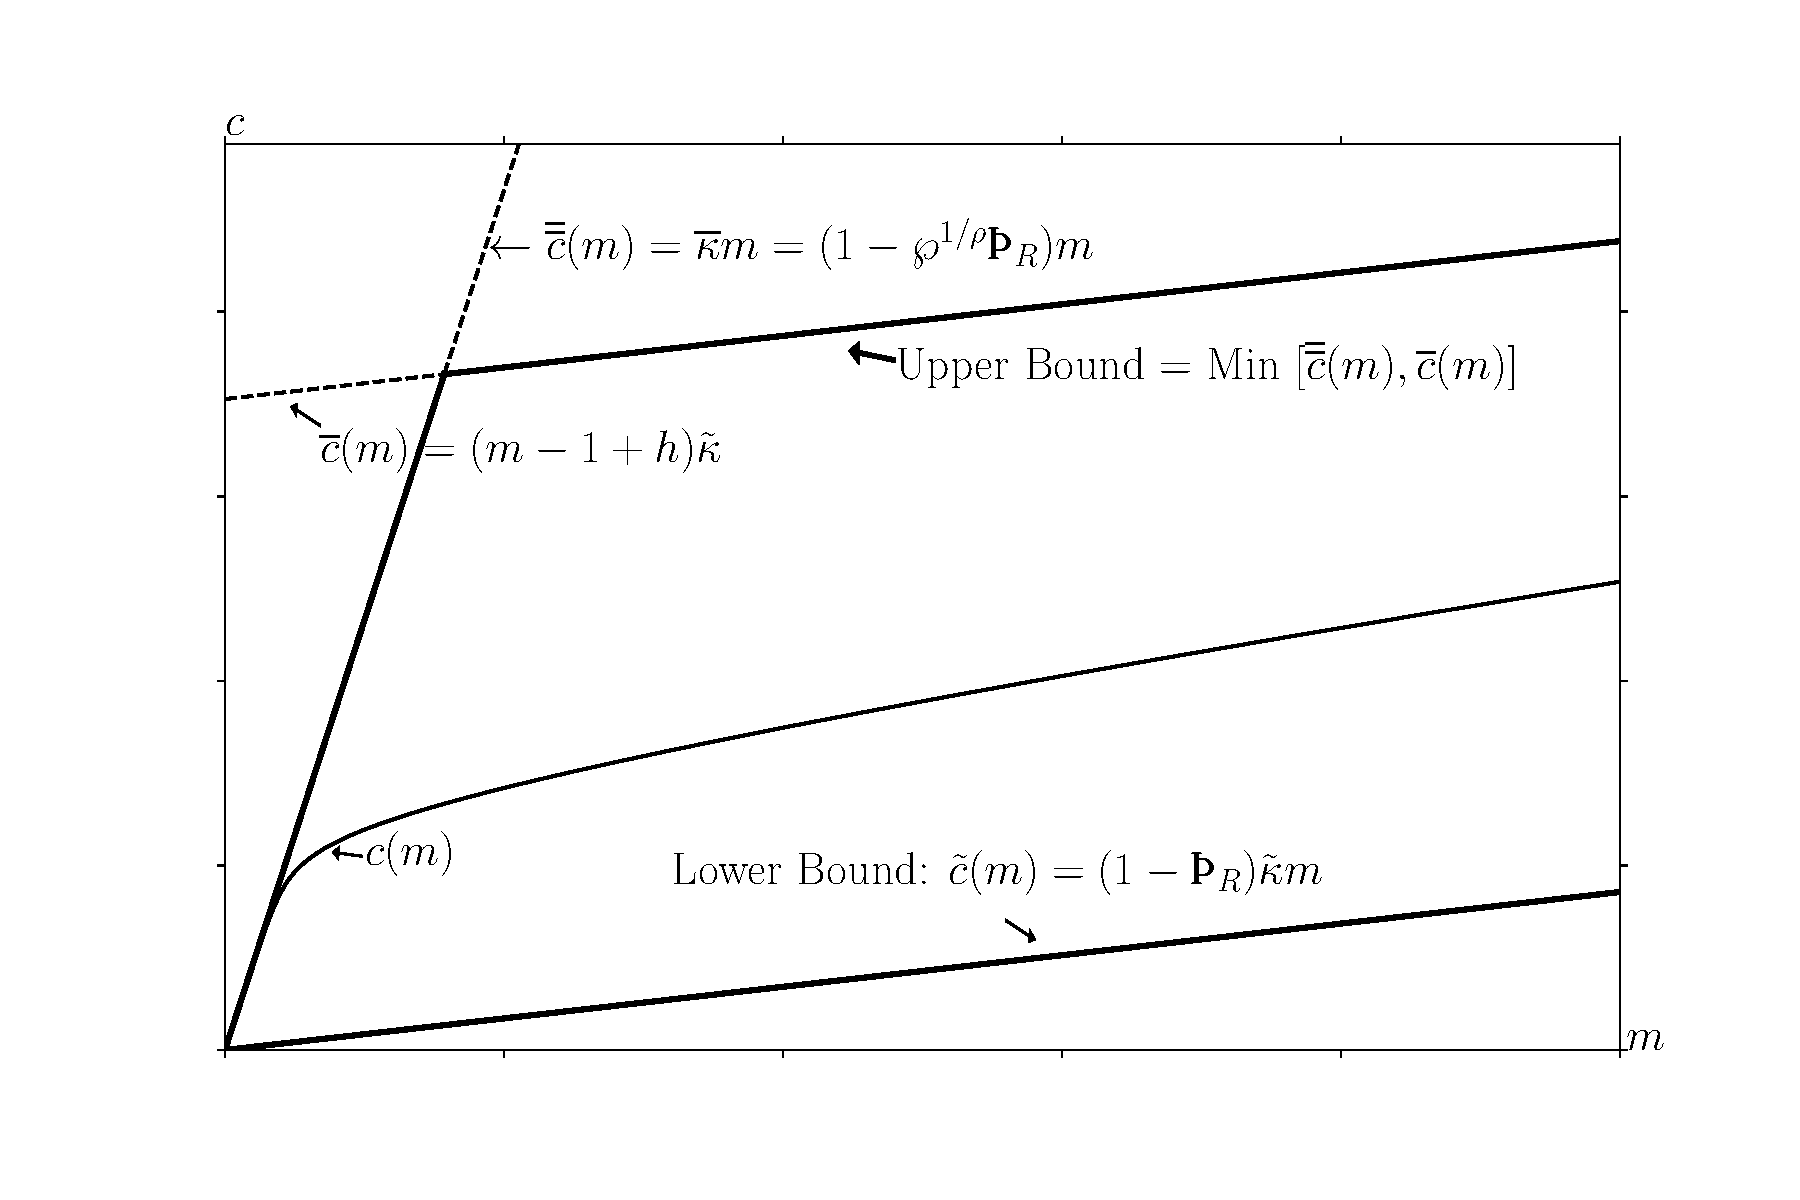
\includegraphics[width=6in]{\FigDir/cFuncBounds}
\caption{Upper and Lower Bounds on The Consumption Function}
\label{fig:cFuncBounds}
\end{figure}


Next we establish the limit of the expected consumption growth factor
as $\mRat_{t} \uparrow \infty$:
\begin{align*}
  \lim_{\mRat_{t} \uparrow \infty} \Ex_{t}[
  \cLevBF_{t+1}/\cLevBF_{t}]  & = \lim_{\mRat_{t} \uparrow \infty} \Ex_{t}[
                                {\PGro}_{t+1} {\cRat}_{t+1}/c_{t}].
\end{align*}

But
\begin{align*}
  \Ex_{t}[{\PGro}_{t+1} {\ushort{\cRat}}_{t+1}/\bar{\cRat_{t}}] \leq \Ex_{t}[{\PGro}_{t+1} {\cRat}_{t+1}/\cRat_{t}] \leq \Ex_{t}[{\PGro}_{t+1} {\bar{\cRat}}_{t+1}/\ushort{\cRat}_{t}]
\end{align*}
and
\begin{equation*}  \label{eq:xttoinfty}
  \lim_{\mRat_t \uparrow \infty} \PGro_{t+1}\ushort{\cFunc}(\mRat_{t+1})/\bar{\cFunc}(\mRat_t) =
  \lim_{\mRat_{t} \uparrow \infty} \PGro_{t+1}\bar{\cFunc}(\mRat_{t+1})/\ushort{\cFunc}(\mRat_t) =
  \lim_{\mRat_{t} \uparrow \infty}\PGro_{t+1} \mRat_{t+1}/\mRat_t,
\end{equation*}
while (for convenience defining $\aFunc(\mRat_{t})=\mRat_{t}-\usual{\cFunc}(\mRat_{t})$), \hypertarget{xtp1toinfty}{}
\begin{align}  \label{eq:xtp1toinfty}
  \lim_{\mRat_{t} \uparrow \infty} \PGro_{t+1} \mRat_{t+1}/\mRat_t  & = \lim_{\mRat_{t} \uparrow \infty}
                                                                  \left(\frac{\Rfree \aFunc(\mRat_t)+{\PGro}_{t+1}\tShkAll_{t+1}}{\mRat_t}\right)
  \\  & = {(\Rfree \DiscFac)}^{1/\CRRA} = \Pat \notag
\end{align}
because $\lim_{\mRat_{t}\uparrow \infty} \aFunc^{\prime}(\mRat)=\PatR$\footnote{This is because $\lim_{\mRat_{t}\uparrow \infty} \aFunc(\mRat_{t})/\mRat_{t}=1-\lim_{\mRat_{t}\uparrow \infty} \usual{\cFunc}(\mRat_{t})/\mRat_{t}=1-\lim_{\mRat_{t}\uparrow \infty}\usual{\cFunc}^{\prime}(\mRat_{t})=\PatR$.} and
$\PGro_{t+1}\tShkAll_{t+1}/\mRat_{t} \leq (\PGro \bar{\pShk} \bar{\tShkEmp}/\pNotZero )/\mRat_{t}$ which
goes to zero as $\mRat_{t}$ goes to infinity.

Hence we have
\begin{equation*}
  {\Pat}  \leq \lim_{\mRat_{t} \uparrow \infty} \Ex_{t}[\cLevBF_{t+1}/\cLevBF_{t}] \leq {\Pat}
\end{equation*}
so as cash goes to infinity, consumption growth approaches its
value $\Pat$ in the perfect foresight model.
% This argument applies equally well to the problem of the restrained consumer, because as $\mRat$ approaches infinity the constraint becomes irrelevant (assuming the \FHWC~holds).

\begin{comment}
  Of course, the constraint never becomes irrelevant if human wealth is
  infinite.  We ruled out infinite human wealth at the beginning of this
  section by assuming $\Rfree> \PGro$.  If this finite human wealth
  condition does not hold, it is possible to show that for any finite
  horizon consumer the marginal propensity to consume approaches the
  finite-horizon perfect foresight MPC as wealth approaches infinity.
  However, as the horizon gets longer, the perfect foresight MPC
  approaches zero.  It can be shown therefore that the limiting MPC for
  the converged consumption function approaches (but never reaches)
  zero.  (This is why we chose $\MinMinMPC=0$ if the \FHWC~fails
  in the proofs above.)
\end{comment}

\hypertarget{LimitsAsmtToZero}{}
\subsection{Limits as \texorpdfstring{$\mRat$}{m} Approaches Zero}\label{subsec:LimitsAsmtToZero}
%\label{subsec:LimitsAsmtToZero} Now consider the limits of behavior as $\mRat_{t}$ gets arbitrarily small.

Equation~\eqref{eq:MaxMPCInv} shows that the limiting value of
$\MaxMPC$ is
\begin{align*}
  \MaxMPC  & = 1-{\Rfree}^{-1}{(\pZero  \Rfree\DiscFac)}^{1/\CRRA}.
\end{align*}

Defining $\eFunc(\mRat)=\cFunc(\mRat)/\mRat$ as before we have
\begin{align*}
  \lim_{m \downarrow 0} \eFunc(\mRat)  & = (1-\pZero^{1/\CRRA}\PatR) = \MaxMPC .
\end{align*}

Now using the continuous differentiability of the consumption function
along with L'H\^opital's rule, we have
\begin{comment}
  \begin{align*}
    \eFunc^{\prime}(\mRat)  & = \mRat^{-1} \usual{\cFunc}^{\prime}(\mRat) - \mRat^{-2} \usual{\cFunc}(\mRat)
    \\ \mRat \eFunc^{\prime}(\mRat)  & = \usual{\cFunc}^{\prime}(\mRat) - \usual{\cFunc}(\mRat)/\mRat
    \\ \usual{\cFunc}^{\prime}(\mRat)  & = \eFunc(\mRat)+ \mRat \eFunc^{\prime}(\mRat)
  \end{align*}
  and since $0<\eFunc(\mRat)<1$ we have
\end{comment}
\begin{align*}
  \lim_{m \downarrow 0} \usual{\cFunc}^{\prime}(\mRat)  & = \lim_{m \downarrow 0}
                                                  \eFunc(\mRat) = \MaxMPC.
\end{align*}

Figure~\ref{fig:mpclimits} confirms that the numerical solution obtains this limit for the MPC as $\mRat$ approaches zero.

For consumption growth, as $\mRat \downarrow 0$ we have
\begin{align*}
  \lim_{\mRat_{t} \downarrow 0} \Ex_{t}\left[\left(\frac{\cFunc({\mRat}_{t+1})}{\cFunc(\mRat_t)}\right){\PGro}_{t+1}\right]
  & > \lim_{\mRat_{t} \downarrow 0} \Ex_{t}\left[\left(\frac{\ushort{\cFunc}({\mathcal{\mathcal{R}}}_{t+1}\aFunc(\mRat_{t})+{%
    \tShkAll}_{t+1})}{\MaxMPC \mRat_{t}}\right){\PGro}_{t+1}\right]  \notag \\
  & = \pZero \lim_{\mRat_{t} \downarrow 0} \Ex_{t}\left[\left(\frac{\ushort{\cFunc}({\mathcal{\mathcal{R}}}_{t+1}\aFunc(\mRat_{t}))}{\MaxMPC \mRat_{t}}\right){\PGro}_{t+1}\right] \\
  & ~~~~~~ + \pNotZero \lim_{\mRat_{t} \downarrow 0}  \Ex_{t}\left[\left(\frac{\ushort{\cFunc}({\mathcal{\mathcal{R}}}_{t+1}\aFunc(\mRat_{t})+
    \tShkEmp_{t+1}/\pNotZero)}{\MaxMPC \mRat_{t}}\right){\PGro}_{t+1}\right]  \\\notag
  & > \pNotZero \lim_{\mRat_{t} \downarrow 0} \Ex_{t}\left[\left(\frac{\ushort{\cFunc}(
    \tShkEmp_{t+1}/\pNotZero)}{\MaxMPC \mRat_{t}}\right){\PGro}_{t+1}\right] \\
  & = \infty \nonumber
\end{align*}
where the second-to-last line follows because  $\lim_{\mRat_{t} \downarrow 0} \Ex_{t}\left[\left(\frac{\ushort{\cFunc}({\mathcal{\mathcal{R}}}_{t+1}\aFunc(\mRat_{t}))}{\MaxMPC \mRat_{t}}\right){\PGro}_{t+1}\right]$ is positive, and the last line follows because the minimum possible realization of $\tShkEmp_{t+1}$ is $\ushort{\tShkEmp}>0$ so the minimum possible value of expected next-period consumption is positive.\footnote{None of the arguments in either of the two prior sections depended on the assumption that the consumption functions had converged.  With more cumbersome notation, each derivation could have been replaced by the corresponding finite-horizon versions.  This strongly suggests that it should be possible to extend the circumstances under which the problem can be shown to define a contraction mapping to the union of the parameter values under which \{\RIC,\FHWC\} hold and \{\FVAC,\WRIC\} hold.  That extension is not necessary for our purposes here, so we leave it for future work.}

\hypertarget{onetarget}{}
\hypertarget{Unique-Stable-Points}{}

\subsection{Unique `Stable' Points}\label{subsec:onetarget}\hypertarget{TheoremTarget}{}

Two theorems, whose substance is described here and whose details are in an appendix, articulate alternative (but closely related) stability criteria for the model.

\subsubsection{`Individual Target Wealth'}\label{subsubsec:mTarget}
One definition of a `stable' point is an $\mTrg$ such that if $\mRat_{t}=\mTrg$, then $\Ex_{t}[\mRat_{t+1}]=\mRat_{t}$.  Existence of such a target turns out to require the {\GICNrm} condition.

\begin{verbatimwrite}{\EqDir/TheoremMTargetIsStable}
\begin{theorem}\label{thm:target}
  For the nondegenerate solution to the problem defined in Section~\ref{subsec:Setup} when {\FVAC}, {\WRIC}, and {\GICNrm} all hold, there exists a unique cash-on-hand-to-permanent-income ratio $\mTrg>0$ such that
  \begin{equation}
    \Ex_t [{\mRat}_{t+1}/\mRat_t] = 1 \mbox{~if~} \mRat_t = \mTrg.
    \label{eq:mTarget}
  \end{equation}
  Moreover, $\mTrg$ is a point of `wealth stablity' in the sense that
  \begin{align}\label{eq:stability}
    \forall {\mRat}_t\in(0,\mTrg),      \,\,& \Ex_t [{\mRat}_{t+1}] > {\mRat}_t  \\
    \forall {\mRat}_t\in(\mTrg,\infty), \,\,& \Ex_t [{\mRat}_{t+1}] < {\mRat}_t. \notag
  \end{align}
  \end{theorem}
\end{verbatimwrite}
\begin{theorem}\label{thm:target}
  For the nondegenerate solution to the problem defined in Section~\ref{subsec:Setup} when {\FVAC}, {\WRIC}, and {\GICNrm} all hold, there exists a unique cash-on-hand-to-permanent-income ratio $\mTrg>0$ such that
  \begin{equation}
    \Ex_t [{\mRat}_{t+1}/\mRat_t] = 1 \mbox{~if~} \mRat_t = \mTrg.
    \label{eq:mTarget}
  \end{equation}
  Moreover, $\mTrg$ is a point of `wealth stablity' in the sense that
  \begin{equation}\begin{gathered}\begin{aligned}\label{eq:stability}
    \forall {\mRat}_t\in(0,\mTrg),      \,\,& \Ex_t [{\mRat}_{t+1}] > {\mRat}_t  \\
    \forall {\mRat}_t\in(\mTrg,\infty), \,\,& \Ex_t [{\mRat}_{t+1}] < {\mRat}_t. \notag
  \end{aligned}\end{gathered}\end{equation}
  \end{theorem}


 \hypertarget{mTargImplicit}{}

 Since $\mRat_{t+1}=(\mRat_{t}-\cFunc(\mRat_{t}))\Rnorm_{t+1}+\tShk_{t+1}$, the implicit equation for $\mTrg$ is
 \begin{align}
  \Ex_{t}[(\mTrg-\cFunc(\mTrg))\Rnorm_{t+1}+\tShk_{t+1}] & = \mTrg \label{eq:mTargImplicit}
\\   (\mTrg-\cFunc(\mTrg))\underbrace{\Rnorm\Ex_{t}[\pShk^{-1}]}_{\equiv \bar{\Rnorm}}+1 & = \mTrg \notag
 \end{align}


 \begin{comment}
 The full proof is in Appendix~\ref{sec:ApndxMTargetIsStable}, but the key points can be made informally here.  Existence of such a point is guaranteed by
 \begin{enumerate}
 \item Existence, continuity, and monotonicity of $\Ex_t [{\mRat}_{t+1}-\mRat_t]$
 \item $\lim_{\mRat_{t}\downarrow 0} \Ex_t [{\mRat}_{t+1}/\mRat_t] > 1 > \lim_{\mRat_{t}\uparrow \infty} \Ex_t [{\mRat}_{t+1}/\mRat_t]$
\item The intermediate value theorem
\end{enumerate}
% which can be differentiated and rearranged to yield\hypertarget{mTargDerImplicit}{}
 \begin{align}
   \bar{\Rnorm}(1-\usual{\cFunc}^{\prime}(\mTrg)) & = 1 \\
   (1-\usual{\cFunc}^{\prime}(\mTrg)) & = \bar{\Rnorm}^{-1} \\
%   1-\bar{\Rnorm}^{-1} & = \usual{\cFunc}^{\prime}(\mTrg). \label{eq:mTargDerImplicit}
 \end{align}

 The fact (cf.\~\eqref{eq:MinMPCDef}) that the minimum value of $\usual{\cFunc}^{\prime}$ is $1-\PatR$ converts~\eqref{eq:mTargDerImplicit} to the inequality $1-\bar{\Rnorm}^{-1} > 1-\PatR$ from which we have
 \begin{align}
      \PGroAdj/\Rfree & > \Pat/\Rfree \notag
\\    1 & > \Pat/\PGroAdj
 \end{align}
 which is the {\GICNrm}; thus, if a stable point exists, it must satisfy the {\GICNrm}.  (The appendix proves that if the {\GICNrm} is satisfied, such a point must exist, and be globally stable).
\end{comment}

 \hypertarget{Collective-Stability}{}
 \subsubsection{Collective Stability and the Expected-Balanced-Growth State}\label{subsubsec:mSteadyState}
 A traditional question in macroeconomic models is whether there is a `balanced growth' equilibrium in which aggregate variables (income, consumption, market resources) all grow forever at the same rate.  For the model here, we have already seen in Figure~\ref{fig:cGroTargetFig} that there is no single $\mRat$ for which $\Ex_{t}[\mRatBF_{t+1}]/\mRatBF_{t} = \Ex_{t}[\cLevBF_{t+1}]/\cLevBF_{t} = \PGro$~for an individual consumer.  Nevertheless, analysis below will show that economies populated by collections of such consumers can exhibit balanced growth in the aggregate.

As an input to that analysis, we show here that if the {\GIC} holds, the problem will have a point of what we call `collective stability' by which we mean that there is some ${\mStE}$ such that, for all $\mRat_{t}>{\mStE}$, $\Ex_{t}[\mRat_{t+1}/\mRat_{t}] < \PGro$, and conversely for $\mRat_{t}<{\mStE}$.  (`Collective' is meant to capture the fact that calculating the expectation of the levels of future $\mLevBF$ and $\pLevBF$ before dividing $\mLevBF$ by $\pLevBF$ is akin to examining aggregate values in a population).

 \hypertarget{balgrostable}{}
\hypertarget{balgrostableSolve}{}

 The critical $\mRat$ will be the value at which $\mRatBF$ growth matches $\PGro$:
  \begin{align}
  \Ex_{t}[\mLevBF_{t+1}]/\mLevBF_{t} & =\Ex_{t}[\pLevBF_{t+1}]/\pLevBF_{t} \notag
    \\  \Ex_{t}[\mRat_{t+1}\PGro\pShk_{t+1}\pLevBF_{t}]/(\mRat_{t}\pLevBF_{t}) & =\Ex_{t}[\pLevBF_{t}\PGro\pShk_{t+1}]/\pLevBF_{t} \notag
    \\ \Ex_{t}\left[\pShk_{t+1}\underbrace{\left((\mRat_{t}-\usual{\cFunc}(\mRat_{t})\Rfree/(\PGro\pShk_{t+1}))+\tShk_{t+1}\right)}_{\mRat_{t+1}}\right]/\mRat_{t} & = 1 \notag
    \\
    \Ex_{t}\left[(\mStE-\usual{\cFunc}(\mBal))\overbrace{\Rfree/\PGro}^{\Rnorm}+\pShk_{t+1}\tShk_{t+1}\right] & = \mBal \notag
\\  (\mStE-\usual{\cFunc}(\mBal))\Rnorm+ 1 & = \mBal \label{eq:balgrostable}
% \\  \aFunc(\mStE+\epsilon)(\Rnorm+\nu)+ 1 & = \mBal+\epsilon
% \\  (\aFunc(\mStE)+\epsilon\aFunc^{\prime})(\Rnorm+\nu)+ 1 & \approx \mBal+\epsilon
% \\  \epsilon\aFunc^{\prime}(\Rnorm+\nu) + \aFunc(\hat{\mRat})\nu & \approx \epsilon
% \\   \nu\aFunc(\hat{\mRat}) & \approx \epsilon\left(1-\aFunc^{\prime}(\Rnorm+\nu)\right)
% \\   \frac{\nu\aFunc(\hat{\mRat})}{\left(1-\aFunc^{\prime}(\Rnorm+\nu)\right)} & \approx \epsilon
\end{align}

The only difference between~\eqref{eq:balgrostable} and~\eqref{eq:mTargImplicit} is the substitution of $\Rnorm$ for $\bar{\Rnorm}$.

  We will refer to $\mStE$ as the problem's Expected-Balanced-Growth State, a term motivated by the fact that an economy composed of consumers all of whom had $\mRat_{t}=\mStE$, \textit{would} exhibit balanced growth if all consumers happened to continually draw permanent and transitory shocks equal to their expected values of 1.0 forever.%\footnote{    \begin{align*}      \Ex_{t}[\mRat_{t+1}/\mRat_{t}|\pShk_{t+1}=\tShk_{t+1}=1] = \PGro \left(\mStE-\cFunc(\mStE)\Rnorm + 1 \right)/\mRat = \PGro    \end{align*}}


%Note that since $\PGroAdj < \PGro$, $\usual{\cFunc}^{\prime}(\mTrg) > \usual{\cFunc}^{\prime}(\mStE)$ which implies that $\mTrg < \mBal$.

Theorem~\ref{thm:MSSBalExists}~formally states the relevant proposition.
  \begin{verbatimwrite}{\EqDir/TheoremMSSBalExists}
\begin{theorem}\label{thm:MSSBalExists}
 For the nondegenerate solution to the problem defined in Section~\ref{subsec:Setup} when {\FVAC}, {\WRIC}, and {\GIC} all hold, there exists a unique pseudo-steady-state cash-on-hand-to-income ratio $\mStE>0$ such that
  \begin{equation}
    \Ex_t [\pShk_{t+1}{\mRat}_{t+1}/\mRat_t] = 1 \mbox{~if~} \mRat_t = \mStE.
    \label{eq:mStE}
  \end{equation}
  Moreover, $\mStE$ is a point of stability in the sense that
  \begin{align}\label{eq:stabilityStE}
    \forall {\mRat}_t\in(0,\mStE),      \,\,& \Ex_{t}[\mLevBF_{t+1}]/\mLevBF_{t} > \PGro \\
    \forall {\mRat}_t\in(\mStE,\infty), \,\,& \Ex_{t}[\mLevBF_{t+1}]/\mLevBF_{t} < \PGro. \notag
  \end{align}
\end{theorem}
\end{verbatimwrite}
\begin{theorem}\label{thm:MSSBalExists}
 For the nondegenerate solution to the problem defined in Section~\ref{subsec:Setup} when {\FVAC}, {\WRIC}, and {\GIC} all hold, there exists a unique pseudo-steady-state cash-on-hand-to-income ratio $\mStE>0$ such that
  \begin{equation}
    \Ex_t [\pShk_{t+1}{\mRat}_{t+1}/\mRat_t] = 1 \mbox{~if~} \mRat_t = \mStE.
    \label{eq:mStE}
  \end{equation}
  Moreover, $\mStE$ is a point of stability in the sense that
  \begin{align}\label{eq:stabilityStE}
    \forall {\mRat}_t\in(0,\mStE),      \,\,& \Ex_{t}[\mLevBF_{t+1}]/\mLevBF_{t} > \PGro \\
    \forall {\mRat}_t\in(\mStE,\infty), \,\,& \Ex_{t}[\mLevBF_{t+1}]/\mLevBF_{t} < \PGro. \notag
  \end{align}
\end{theorem}


%the sense in which $\mStE$ is a `target' is less obvious than that for $\mtarg$; a full justification of this terminology must await the macroeconomic analysis below.  a glimpse of the idea is can be seen by noting that, for an economy whose entire population of consumers in period $t$ all had $\mRat_{t} = \mBal$, the ratio of the aggregate values $\mlevbf_{t+1}= \int \mlevbf_{t+1}$ to $\plevbf_{t+1}= \int \plevbf_{t+1}$ next period would be $\mlevbf_{t+1}/\plevbf_{t+1}=\mbal$ so that, at least between those two periods, the economy would exhibit stability.  indeed, if we turned off the idiosyncratic shocks,

The proofs of the two theorems are almost completely parallel; to save space, they are relegated to Appendix~\ref{sec:ApndxMTargetIsStable}.  In sum, they involve three steps:

\begin{enumerate}
\item Existence and continuity of $\Ex_{t}[\mRat_{t+1}/\mRat_{t}]$ or $\Ex_{t}[\mRat_{t+1}\pShk_{t+1}/\mRat_{t}]$
  \begin{itemize}
    \item This follows from existence and continuity of the constituents
    \end{itemize}
  \item Existence of the equilibrium point
    \begin{itemize}
    \item This follows from the upper and lower bound limiting MPC's, existence and continuity, and the Intermediate Value Theorem
    \end{itemize}
  \item Monotonicity of $\Ex_{t}[{\mRat}_{t+1}-\mRat_{t}]$ or $\Ex_{t}[{\mRat}_{t+1}\pShk_{t+1}-\mRat_{t}]$
    \begin{itemize}
    \item This follows from concavity of the consumption function
    \end{itemize}
\end{enumerate}

\subsubsection{Example Where There Is An Expected-Balanced-Growth
  \texorpdfstring{$\mStE$}{m} State But No Target}

Because the equations defining target and pseudo-steady-state $\mRat$,~\eqref{eq:mTargImplicit} and~\eqref{eq:balgrostable}, differ only by substitution of $\Rnorm$ for $\bar{\Rnorm}=\Rnorm \Ex[\pShk^{-1}]$, if there are no permanent shocks ($\pShk \equiv 1$), the conditions are identical.  For many parameterizations (e.g., under the baseline parameter values used for constructing figure~\ref{fig:cGroTargetFig}), $\Trg{\mRat}$ and $\StE{\mRat}$ will not differ much.

An illuminating exception is exhibited in Figure~\ref{fig:GICNrmFailsButGICRawHolds}, which modifies the baseline parameter values by quadrupling the variance of the permanent shocks, enough to cause failure of the \GICNrm; now there is no target wealth level $\Trg{\mRat}$ ($\cFunc(m)$ remains everywhere below the level that would keep expected $\mRat$ constant).


\renewcommand{\figFile}{GICNrmFailsButGICRawHolds}
\hypertarget{\figFile}{}
 % Store the tex for standalone compilation
\begin{figure}[tbp]
\centerline{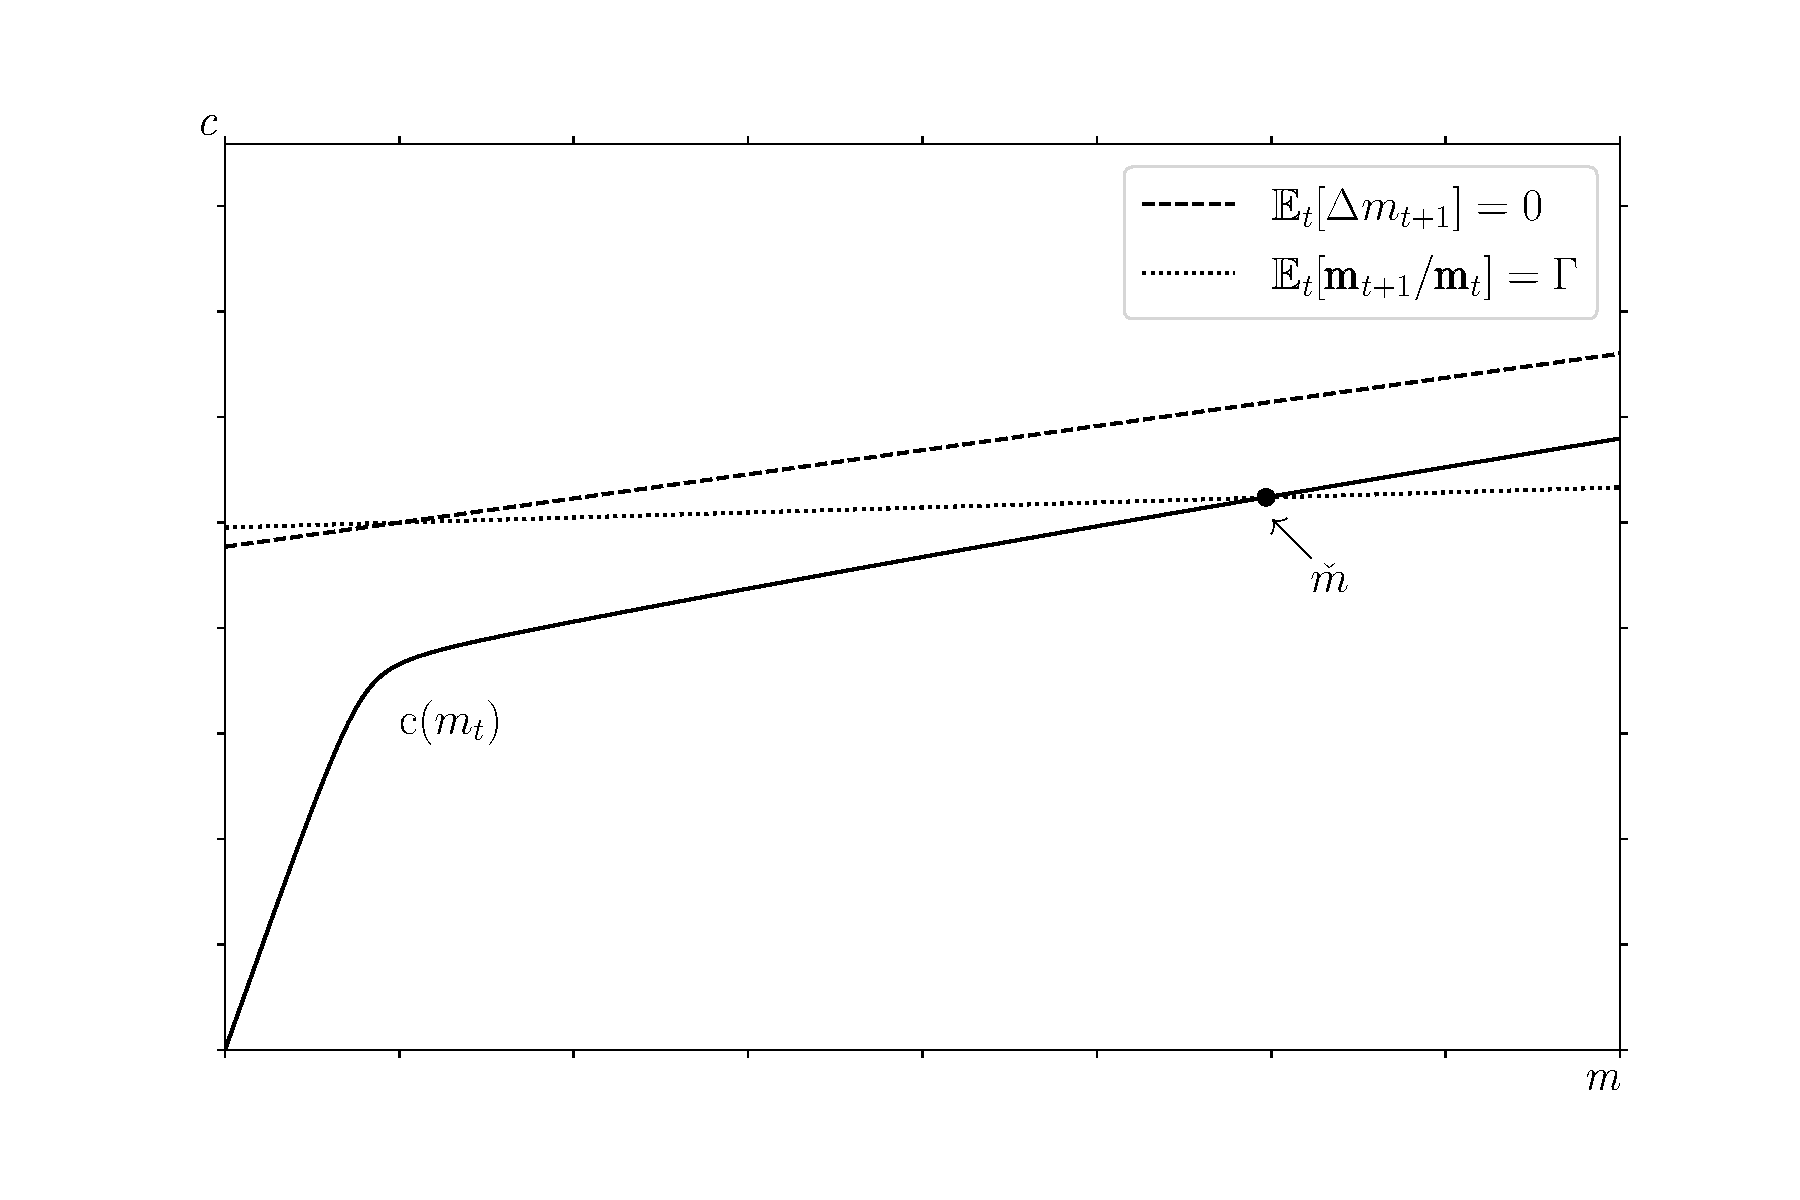
\includegraphics[width=6in]{\FigDir/GICNrmFailsButGICRawHolds}}
\caption{\{\FVAC,\GICRaw,\cncl{\GICNrm}\}: No $\Trg{\mRat}$ Exists But $\StE{\mRat}$ Does}
\label{fig:GICNrmFailsButGICRawHolds}
\end{figure}


The pseudo-steady-state still exists because it turns off realizations of the permanent shock.  But an aggregate balanced growth equilibrium can exist even when realizations of the permanent shock are not turned off, and instead implemented exactly as specified in the model.  The key insight can be understood by considering the evolution of an economy that starts, at date $t$, with the entire population at $\mRat_{t}=\StE{\mRat}$, but then evolves according to the model's assumed dynamics between $t$ and $t+1$.  Equation~\eqref{eq:balgrostable} will still hold, so for this first period, at least, the economy will exhibit balanced growth: the growth factor for aggregate $\mRatBF$ will match the growth factor for permanent income $\PGro$.  It is true that there will be people for whom $\bRat_{t+1}=\aRat_{t}\Rfree/(\PGro\pShk_{t+1})$ is boosted by a small draw of $\pShk_{t+1}$.  But their contribution to the aggregate variable is given by $\bRatBF_{t+1}=\bRat_{t+1}\pShk_{t+1}$, so their $\bRatBF_{t+1}$ is reweighted by an amount that exactly unwinds that boosting.

The surprising consequence is that, if the {\GICRaw}~holds but the {\GICNrm}~fails, it is possible to construct an aggregate economy composed of consumers all of whom have target wealth of $\Trg{\mRat}=\infty$, but in which the aggregate economy still exhibits balanced growth with a finite ratio of aggregate wealth to income.  %(For an example, see the software archive for the paper).

This is a good introduction to a more explicit discussion of aggregation.


\begin{comment}
\subsubsection{Example Where There Is A Solution Without A Target}\label{subsubsec:FVACnotGIC}

To build intuition, it is useful to describe an example in which a nondegenerate solution exists but a target $\mTrg$ does not.  An example that satisfies the combination \FVAC~and~\cncl{\GICNrm} is depicted in Figure~\ref{fig:FVACnotGIC}.  The consumption function is shown along with the $\Ex_{t}[\Delta \mRat_{t+1}]=0$ locus that identifies the `sustainable' level of spending at which $\mRat$ is expected to remain unchanged.  The diagram suggests a fact that is confirmed by deeper analysis: Under the depicted configuration of parameter values (see the code for details), the consumption function never reaches the $\Ex_{t}[\Delta \mRat_{t+1}]=0$ locus; indeed, when the \RIC~holds but the \GICNrm~does not, the consumption function's limiting slope $(1-\Pat/\Rfree)$ is shallower than that of the sustainable consumption locus $(1-\PGroAdj/\Rfree)$,\footnote{This is because $\Ex_{t}[\mRat_{t+1}]=\Ex_{t}[\Rnorm_{t+1}(\mRat_{t}-\cRat_{t})]+1$; solve $\mRat = (\mRat - \cRat)\Rnorm \InvEpShkInv^{-1}+1$ for $\cRat$ and differentiate.}  so the gap between the two \textit{increases} with $\mRat$ in the limit.  Although a nondegenerate consumption function exists, a target level of $\mRat$ does not (or, rather, the target is $\mRat=\infty$), because no matter how wealthy a consumer becomes, the consumer will always spend less than the amount that would keep $\mRat$ stable (in expectation).

\renewcommand{\figFile}{FVACnotGIC}
\hypertarget{\figFile}{}
\hypertarget{FVACnotGIC}{}
\begin{figure}[tbp]
\centerline{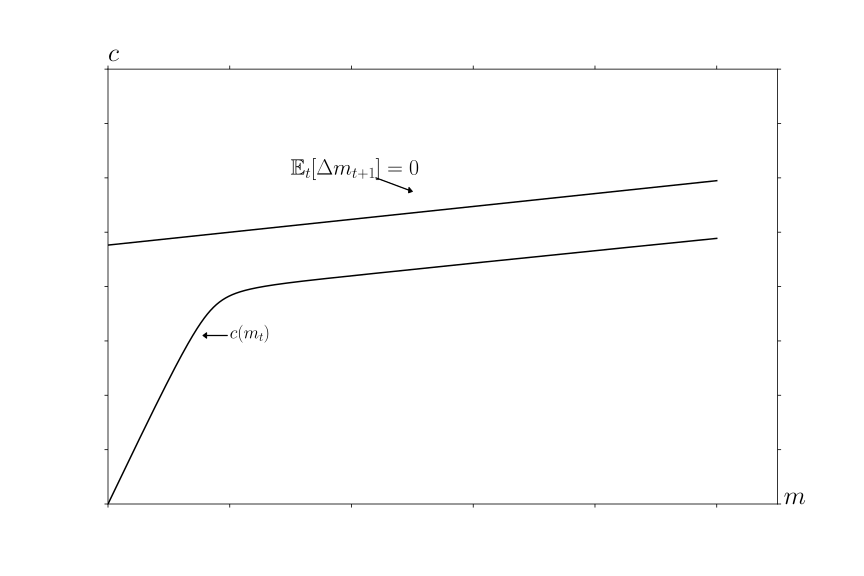
\includegraphics[width=6in]{\FigDir/FVACnotGIC}}
\caption{Example Solution under \{\FVAC,\cncl{\GICNrm}\}}
\label{fig:FVACnotGIC}
\end{figure}


\hypertarget{cGroLTpGro}{}
% \subsection{Expected Consumption Growth at $\hat{m}$ Is Less than  Expected Permanent Income Growth}



\label{subsec:expcgrowth} Figure~\ref{fig:cGroTargetFig} shows that at the value of $\mRat=\mStE$ where expected growth in market resources $\Ex_{t}[\mLevBF_{t+1}/\mLevBF_{t}]$ matches expected growth in permanent income $\PGro$, the expected growth rate of consumption $\Ex_{t}[\cLevBF_{t+1}/\cLevBF_{t}]$ is lower than $\PGro.$

A second-order expansion of next period's consumption function around $\hat{\mRat}$ yields:
\begin{align*}
  \usual{\cFunc}(\mRat_{t+1}) & \approx \usual{\cFunc}(\hat{\mRat})+\usual{\cFunc}^{\prime}(\hat{\mRat})(\mRat_{t+1}-\hat{\mRat})+\usual{\cFunc}^{\prime\prime}(\hat{\mRat})(1/2)(\mRat_{t+1}-\hat{\mRat})^{2}
%  \\ & < \usual{\cFunc}(\hat{\mRat})+\usual{\cFunc}^{\prime}(\hat{\mRat})(\mRat_{t+1}-\hat{\mRat})
\end{align*}
where the inequality holds because strict concavity of the consumption function means that $\usual{\cFunc}^{\prime\prime}(\hat{\mRat})$ is strictly negative, and of course $(1/2)(\mRat_{t+1}-\hat{\mRat})^{2}>0$.

Expected consumption growth is therefore
\begin{align}
  \Ex_{t}\left[\frac{{\PGro}_{t+1} \usual{\cFunc}({\mRat}_{t+1})}{\usual{\cFunc}(\mRat_{t})}
  \right]  & \lesssim \PGro \left(\frac{
             \usual{\cFunc}(\mStE)+\usual{\cFunc}^{\prime}(\mBal)\overbrace{\Ex_{t}[\pShk_{t+1}{\mRat}_{t+1}-\mBal]}^{=0~\text{~from~\eqref{eq:balgrostable}}}}{\usual{\cFunc}(\mBal)}\right)  = \PGro \nonumber \\
\end{align}

In fact, the $\mRat_{t}$ for which $Ex_{t}[\aRatBF_{t+1}/\aRatBF_{t}] = \PGro$ is yet another slightly different value of $\mRat.$
\end{comment}

\begin{comment}
\begin{align}
  \PGro & = \Ex_{t}[\aRatBF_{t+1}/\aRatBF_{t}]
\\      & = \Ex_{t}[\PGro_{t+1}(\mRat_{t+1}-\cFunc(\mRat_{t+1}))\pLevBF_{t}/\aRat_{t}\pLevBF_{t}]
\\   1   & = \Ex_{t}[\pShk_{t+1}(\mRat_{t+1}-\cFunc(\mRat_{t+1}))/\aRat_{t}]
  \\   \aRat_{t}   & = \Ex_{t}[\pShk_{t+1}(\mRat_{t+1}-\cFunc(\mRat_{t+1}))]
  \\ & = \Rnorm \aRat_{t} + 1 - \Ex_{t}[\pShk_{t+1}\cFunc(\aRat_{t}\Rnorm_{t+1}+\tShk_{t+1})]
%\\ & \approx \Rnorm \aRat_{t} + 1 - \Ex_{t}[\pShk_{t+1}\left(\cFunc(\Rnorm \aRat_{t}+1)+\cFunc^{\prime}(\grave{\aRat})(\aRat_{t+1}-\grave{\aRat}\right)]
\end{align}
\end{comment}


\begin{comment}
\begin{align}
  \Ex_{t}\left[\frac{{\PGro}_{t+1} \usual{\cFunc}({\mRat}_{t+1})}{\usual{\cFunc}(\mRat_{t})}
  \right]  & < \Ex_{t}\left[\left(\frac{{\PGro}_{t+1}
             (\usual{\cFunc}(\mStE)+\usual{\cFunc}^{\prime}(\mBal)({\mRat}_{t+1}-\mBal))}{\usual{\cFunc}(\mBal)}\right)\right]  \nonumber \\
           & = \Ex_{t}\left[{\PGro}_{t+1} \left(1+\left(\frac{\usual{\cFunc}^{\prime}(\mStE)}{%
             \usual{\cFunc}(\mStE)}\right)({\mRat}_{t+1}-\mBal)\right)\right]  \nonumber  \\
           & = \PGro + \left(\frac{\usual{\cFunc}^{\prime}(\mStE)}{\usual{\cFunc}(\mBal)}\right)\Ex_{t}\left[ {\PGro}_{t+1}\left((\Rfree/{\PGro}_{t+1})(\mBal-\cFunc(\mBal))-\mBal\right)\right]  \nonumber \\
             & = \PGro + \left(\frac{\usual{\cFunc}^{\prime}(\mStE)}{\usual{\cFunc}(\mBal)}\right)\Ex_{t}\left[ \Rfree(\mBal-\cFunc(\mBal))+1-\PGro\mBal\right]  \nonumber \\
           & = \PGro + \left(\frac{\usual{\cFunc}^{\prime}(\mStE)}{\usual{\cFunc}(\mBal)}\right)\left[
             \Ex_{t}[ \PGro_{t+1}]\underbrace{\Ex_{t}[
             {\mRat}_{t+1}-\mStE]}_{=0}+\mbox{cov}_{t}( {\PGro}_{t+1},{\mRat}_{t+1})\right]
             \label{eq:covcgrow}
\end{align}
and since $\mRat_{t+1} = (\Rfree/\PGro_{t+1}) \aFunc(\mStE)+\tShkAll_{t+1}$ and
$\aFunc(\mStE)>0$ it is clear that
cov$_{t}({\PGro}_{t+1},{\mRat}_{t+1})<0$ which implies that
the entire term added to $\PGro$ in~\eqref{eq:covcgrow} is negative, as
required.

Strict concavity of the consumption function implies that if $\Ex_{t}[{\mRat}_{t+1}] = \mTrg = \mRat_{t}$ then
\begin{align}
  \Ex_{t}\left[\frac{{\PGro}_{t+1} \usual{\cFunc}({\mRat}_{t+1})}{\usual{\cFunc}(\mRat_{t})}
  \right]  & < \Ex_{t}\left[\left(\frac{{\PGro}_{t+1}
             (\usual{\cFunc}(\mTrg)+\usual{\cFunc}^{\prime}(\mTrg)({\mRat}_{t+1}-\mTrg))}{\usual{\cFunc}(\mTrg)}\right)\right]  \nonumber \\
           & = \Ex_{t}\left[{\PGro}_{t+1} \left(1+\left(\frac{\usual{\cFunc}^{\prime}(\mTrg)}{%
             \usual{\cFunc}(\mTrg)}\right)({\mRat}_{t+1}-\mTrg)\right)\right]  \nonumber  \\
           & = \PGro + \left(\frac{\usual{\cFunc}^{\prime}(\mTrg)}{\usual{\cFunc}(\mTrg)}\right)\Ex_{t}\left[ {\PGro}_{t+1}\left({\mRat}_{t+1}-\mTrg\right)\right]  \nonumber \\
           & = \PGro + \left(\frac{\usual{\cFunc}^{\prime}(\mTrg)}{\usual{\cFunc}(\mTrg)}\right)\left[
             \Ex_{t}[ \PGro_{t+1}]\underbrace{\Ex_{t}[
             {\mRat}_{t+1}-\mTrg]}_{=0}+\mbox{cov}_{t}( {\PGro}_{t+1},{\mRat}_{t+1})\right]
             \label{eq:covcgrow}
\end{align}
and since $\mRat_{t+1} = (\Rfree/\PGro_{t+1}) \aFunc(\mTrg)+\tShkAll_{t+1}$ and
$\aFunc(\mTrg)>0$ it is clear that
cov$_{t}({\PGro}_{t+1},{\mRat}_{t+1})<0$ which implies that
the entire term added to $\PGro$ in~\eqref{eq:covcgrow} is negative, as
required.

\hypertarget{dcgdxneg}{}
\subsection{Is Expected Consumption Growth a Declining Function of $\mRat_{t}$?}
\label{subsec:dcgdxneg}

Figure~\ref{fig:cGroTargetFig} depicts the expected consumption growth factor as a strictly
declining function of the cash-on-hand ratio. To investigate this,
define
\begin{align*}
  \pmb{\Upsilon}(\mRat_{t})  & \equiv  \PGro_{t+1} \usual{\cFunc}(\Rnorm_{t+1}\aFunc(\mRat_{t})+\tShkAll_{t+1})/\usual{\cFunc}(\mRat_{t})  = \cLevBF_{t+1}/\cLevBF_{t}
\end{align*}
and the proposition in which we are interested is
\begin{align*}
  (d/d\mRat_{t})\Ex_{t}[\underbrace{\pmb{\Upsilon}(\mRat_{t})}_{\equiv \pmb{\Upsilon}_{t+1}}]  & < 0
\end{align*}
or differentiating through the expectations operator, what we want is
\begin{align}
  \Ex_{t}\left[\PGro_{t+1} \left(\frac{\usual{\cFunc}^{\prime}(\mRat_{t+1})\Rnorm_{t+1}\aFunc^{\prime}(\mRat_{t})\usual{\cFunc}(\mRat_{t})-\usual{\cFunc}(\mRat_{t+1})\usual{\cFunc}^{\prime}(\mRat_{t})}{\usual{\cFunc}(\mRat_{t})^{2}}\right)\right]  & < 0 \label{eq:kappaPrimeLT0}.
\end{align}

Appendix~\ref{sec:ApndxCGrowthDeclines} shows that the proposition holds true if there are only transitory (and no permanent) shocks.  The software archive associated with this paper contains an example in which exotic interactions between permanent shocks and extreme curvature that occurs with very small $\pZero$ generate a (small) region where the proposition does not hold.  In practice, for plausible parametric choices (and in models without an artificial liquidity constraint), $\Ex_{t}[\pmb{\Upsilon}_{t+1}^{\prime}]<0$ should generally hold.

\end{comment}

\hypertarget{The-Aggregate-and-Idiosyncratic-Relationship-Between-Consumption-Growth-and-Income-Growth}{}
\section{The Aggregate and Idiosyncratic Relationship Between
  Consumption Growth and Income Growth}

%A large (infinite) collection of small (infinitesimal) buffer-stock consumers with identical parameter values can be thought of as a subset of the population within a single country (say, members of a given education or occupation group), or as the whole population in a small open economy with an exogenous (constant) interest rate.\footnote{It is also possible, and only slightly more difficult, to solve for the steady-state of a closed-economy version of the model where the interest rate is endogenous.}

Until now for convenience we have assumed infinite horizons, with the implicit understanding that Poisson mortality could be handled by adjusting the effective discount factor for mortality.  On that basis, Section~\ref{subsec:cGroEqPGroIndQ} continues to omit mortality.  But a reason for explicitly introducing mortality will appear at the end of Section~\ref{subsec:cGroEqPGroQ}, so implications of alternative assumptions about mortality are briefly examined in Section~\ref{sec:Mortality-And-Redistribution}.

Formally, assume a continuum of \textit{ex ante} identical households on the unit interval, with constant total mass normalized to one and indexed by $i \in [0,1]$, all behaving according to the model specified above.  Szeidl~\citeyearpar{szeidlInvariant} proves that whenever the {\GIC} holds such a population will be characterized by invariant distributions of $\mRat$, $\cRat$, and $\aRat$;\footnote{\cite{szeidlInvariant}'s equation (9), in our notation, is:
  \begin{align*}
    \Ex \log \Rfree (1-\MPC) < \Ex \log \PGro \pShk
    \\  \Ex \log \Rfree \PatR    < \Ex \log \PGro \pShk
\\ \log \PatPGro < \Ex \log \pShk
  \end{align*}
  and under our assumption that $\log \pShk \sim \mathcal{N}(-\sigma^{2}_{\pShk}/2,\sigma^{2}_{\pShk})$ we can exponentiate both sides to obtain the GIC, $\PatPGro < 1$.  If the permanent income shocks are not lognormally distributed, the expression must be tested in Szeidl's original form.
} designate these $\mathcal{F}^{\mRat}$, $\mathcal{F}^{\aRat}$, and $\mathcal{F}^{\cRat}$.%\footnote{Szeidl's proof supplants simulation evidence of ergodicity that appeared in an earlier version of this paper.}


\hypertarget{Consumption-and-Income-Growth-at-the-Household-Level}{}
\subsection{Consumption and Income Growth at the Household Level}\label{subsec:cGroEqPGroIndQ}

The operator $\Mean\left[\bullet\right]$ yields the mean of its argument in the population, as distinct from the expectations operator $\Ex\left[\bullet\right]$ used above, which represents beliefs about the future.

In a converged economy, an economist with a microeconomic dataset could calculate the average consumption growth rate as:
\begin{align*}
  \Mean\left[\Delta \log \cLevBF_{t+1}\right]  & = \Mean\left[ \log {\cRat}_{t+1}\pLevBF_{t+1} - \log c_{t}\pLevBF_{t}\right]  \notag \\
%                                               & = \Mean\left[ \log \pLevBF_{t+1}- \log \pLevBF_{t} + \log {\cRat}_{t+1} - \log c_{t}\right]  \notag \\
                                               & = \Mean\left[ \log \pLevBF_{t+1}- \log \pLevBF_{t}\right] + \Mean\left[ \log {\cRat}_{t+1} - \log c_{t}\right]  \notag \\
                                               & = (\gamma - \sigma^{2}_{\pshk}/2) + \Mean[\log \cRat_{t+1} - \log \cRat_{t}] \\
                                               & = (\gamma - \sigma^{2}_{\pshk}/2)
\end{align*}
where $\gamma=\log \PGro$ and the last equality follows because the invariance of
 $\mathcal{F}^{\cRat}$ (\cite{szeidlInvariant}) means that $\Mean\left[ \log
  {\cRat}_{t+n}\right] = \Mean\left[ \log
  c_{t}\right]$.  Thus, the same {\GIC} that guaranteed the existence of an `individual pseudo-steady-state' value of $\mRat$ at the microeconomic level guarantees both that there will be an invariant distribution of the population across values of the model variables and that in that invariant distribution the mean growth rates of all idiosyncratic variables are the same (see~\cite{szeidlInvariant} for details).

\hypertarget{Growth-Rates-of-Aggregate-Income-and-Consumption}{}
\subsection{Balanced Growth of Aggregate Income, Consumption, and Wealth}\label{subsec:cGroEqPGroQ}

%Attanasio and Weber~\citeyearpar{aw95} point out that concavity of the consumption function can imply that it is quantitatively important to distinguish between the growth rate of average consumption and the average growth rate of  consumption.\footnote{Since we assume number of the households are   normalized to 1, aggregate and average variables are identical.}  We have just examined the average growth rate; we now examine the growth rate of the average.

Using boldface capital letters for aggregates, the growth factor for aggregate income is:
\begin{align*}
  \YLevBF_{t+1}/\YLevBF_{t}  & = \Mean\left[\tShkAll_{t+1}\PGro \pShk_{t+1}\pLevBF_{t}\right]/\Mean\left[\pLevBF_{t}\tShkAll_{t}\right]  \\
                             & = \PGro
\end{align*}
because of the independence assumptions we have made about $\tShkAll$ and $\pShk$.

\begin{comment}
From the perspective of period $t$, %current aggregate assets are nonstochastic, $\BLevBF_{t}=\Mean[b_{t} \pLevBF_{t}]$, but next period's assets are stochastic,
\begin{align*}
  \BLevBF_{t+1} & = \Mean[b_{t+1} \pLevBF_{t+1}]
  \\              & = \PGro \Mean[a_{t}(\Rfree/(\PGro\pShk_{t+1}))\pShk_{t+1}\pLevBF_{t}]
  \\              & = \PGro \Mean[a_{t}\Rnorm\pLevBF_{t}]
  \\              & = \PGro \Mean[(\mRat_{t}-\cFunc(\mRat_{t}))\Rnorm\pLevBF_{t}]
  \\              & = \PGro \Mean[(\bRat_{t}+\tShk_{t}-\cFunc(\bRat_{t}+\tShk_{t}))\Rnorm\pLevBF_{t}]
\end{align*}
\end{comment}

From the perspective of period $t$, %current aggregate assets are nonstochastic, $\ALevBF_{t}=\Mean[a_{t} \pLevBF_{t}]$, but next period's assets are stochastic,
\begin{align*}
  \ALevBF_{t+1} & = \Mean[a_{t+1} \pLevBF_{t+1}]
  \\              & = \PGro \Mean[(a_{t}+(a_{t+1}-a_{t}))\pLevBF_{t}\pShk_{t+1}]
  \\              & = \PGro \left(\underbrace{\Mean[a_{t}\pLevBF_{t}\pShk_{t+1}]}_{=\ALevBF_{t}}+\underbrace{\Mean[(a_{t+1}-a_{t})]}_{=0~(\text{\cite{szeidlInvariant}})}\Mean[\pLevBF_{t}\pShk_{t+1}]+\cov_{t}(a_{t+1}-a_{t},\pLevBF_{t}\pShk_{t+1})\right)
  \\ \ALevBF_{t+1}/\ALevBF_{t}                    & = \PGro \left(1+\frac{\cov(a_{t+1},\pLevBF_{t}\pShk_{t+1})}{\Mean[a_{t}\pLevBF_{t}]}\right)
\end{align*}
Unfortunately, the covariance term in the numerator, while generally small, will not in general be zero.  This is because the realization of the permanent shock $\pShk_{t+1}$ has a nonlinear effect on $\aRat_{t+1}$.
\begin{comment}
\begin{align}
  \aFunc(\mRat_{t+1}) & \approx \aFunc(\mRat_{t})+\aFunc^{\prime}(\mRat_{t})(m_{t+1}-\mRat_{t})
\\ \cov_{t}(a_{t+1}-a_{t},\pLevBF_{t}\pShk_{t+1}) & \approx \cov_{t}\left( \aFunc^{\prime}(\mRat_{t})(m_{t+1}-\mRat_{t}),\pShk_{t+1} \pLevBF_{t})
\end{align}
\end{comment}
Matters are simpler if there are no permanent shocks; see Appendix~\ref{sec:ApndxCGroIsPGro} for a proof that in that case the growth rate of assets (and other variables) does eventually converge to the growth rate of aggregate permanent income.

One way of thinking about the problem here is that it may reflect the fact that, under our assumptions, permanent income $\pLevBF$ does not have an ergodic distribution; its distribution of becomes forever wider over time, because our consumers never die and each immortal person is perpetually subject to symmetric shocks to their $\log \pLevBF$.

This is why we need to introduce mortality.


\hypertarget{Mortality-And-Redistribution}{}
\subsection{Mortality and Redistribution}\label{sec:Mortality-And-Redistribution}

Most heterogeneous-agent models incorporate a constant positive probability of death, following~\cite{blanchardFinite}.  In such a Blanchardian model, for probabilities of death that exceed a threshold that depends on the size of the permanent shocks,~\cite{cstwMPC} show that the limiting distribution of permanent income has a finite variance, which is a useful step in the direction of taming the problems caused by an unbounded distribution of $\pLevBF$.  Numerical results in that paper confirm the intuition that, under appropriate impatience conditions, balanced growth arises (though a formal proof remains elusive).

Even with those (numerical) results in hand, the centrality of mortality assumptions to the existence and nature of steady states requires them to be discussed briefly here.

\hypertarget{Blanchard-Lives}{}
\subsubsection{Blanchard Lives}
\cite{blanchardFinite} assumes the existence of an annuitization scheme in which estates of dying consumers are redistributed to survivors in proportion to survivors' wealth, giving the recipients a higher effective rate of return. This treatment has several analytical advantages, most notably that the effect of mortality on the time preference factor is the exact inverse of its effect on the (effective) interest factor:  If the probability of remaining alive is $\Alive$, then assuming that no utility accrues after death makes the effective discount factor $\hat{\DiscFac}=\DiscFac\Alive$, while the enhancement to the rate of return from the annuity scheme yields an effective interest rate of $\hat{\Rfree}/\Alive$ (recall that because of Poisson mortality, the average wealth of the two groups is identical).  Combining these, the effective patience factor in the new economy $\hat{\Pat}$ is unchanged from its value in the infinite horizon model:% chktex 2
\begin{equation}
  \hat{\Pat} \equiv {\left(\DiscFac \Alive \Rfree / \Alive\right)}^{1/\CRRA} = {\left(\Rfree \DiscFac\right)}^{1/\CRRA} \equiv \Pat.
\end{equation}

The only adjustments this requires to the analysis from prior parts of this paper are therefore to the few elements that involve a role for $\Rfree$ distinct from its contribution to $\Pat$ (principally, the {\RIC}).  %These would need to be adjusted to incorporate in interest factor with a higher rate of return.  %For example, the {\RIC}~($\Pat/(\Rfree /\Alive) < 1$) will be somewhat easier to satisfy because $\Rfree/\Alive > \Rfree$.

The numerical finding that the covariance term above is approximately zero allows us to conclude again that the key requirement for aggregate balanced growth is presumably the {\GICRaw}.

\hypertarget{Modigliani-Lives}{}
\subsubsection{Modigliani Lives}

\cite{blanchardFinite}'s innovation was useful not only for the insight it provided but also because the principal alternative, the Life Cycle model of~\cite{modiglianiWealth}, was computationally challenging given the then-available technologies. Aside from its (considerable) conceptual value, there is no need for Blanchard's analytical solution today, when serious modeling incorporates uncertainty, constraints, and other features that rule out analytical solutions anyway.% chktex 2  %Modern models can can easily handle assumptions more realistic than Blanchard's about the disposition of assets at death.

The simplest alternative to Blanchard's mortality is to follow Modigliani in assuming that any wealth remaining at death occurs accidentally (not implausible, given the robust finding that for the great majority of households, bequests amount to less than 2 percent of lifetime earnings,~\cite{hendricksBequests,hendricksSmallBequests}).

Even if bequests are accidental, a macroeconomic model must make some assumption about how they are disposed of: As windfalls to heirs, estate tax proceeds, etc. We again consider the simplest choice, because it again represents something of a polar alternative to Blanchard: Without a bequest motive, there are no behavioral effects of a 100 percent estate tax; we assume such a tax is imposed and that the revenues are effectively thrown in the ocean; the estate-related wealth effectively vanishes from the economy.

The chief appeal of this approach is the simplicity of the change it makes in the condition required for the economy to exhibit a balanced growth equilibrium.  If $\Alive$ is the probability of remaining alive, the condition changes from the plain {\GIC} to a looser mortality-adjusted {\GIC}:
\hypertarget{GICMrt}{}
\begin{align}
  \Alive  \Pat_{\PGro} & < 1. \label{eq:GICMrt}
\end{align}

With no income growth, the condition required to prohibit unbounded growth in aggregate wealth would be the condition that prevents the per-capita wealth to income ratio of surviving consumers from growing faster than the rate at which mortality diminishes their collective population.  With income growth, the aggregate wealth-to-income ratio will head to infinity only if a cohort of consumers is patient enough to make the desired rate of growth of wealth fast enough to counteract combined erosive forces of mortality and productivity.


\hypertarget{Conclusions}{}
\section{Conclusions}

Numerical solutions to optimal consumption problems, in both life cycle and infinite horizon contexts, have become standard tools since the first reasonably realistic models were constructed in the late 1980s. One contribution of this paper is to show that finite horizon (`life cycle') versions of the simplest such models, with assumptions about income shocks (transitory and permanent) dating back to~\cite{friedmanATheory} and standard specifications of preferences --- and without plausible (but computationally and mathematically inconvenient) complications like liquidity constraints --- have attractive properties (like continuous differentiability of the consumption function, and analytical limiting MPC's as resources approach their minimum and maximum possible values).%, and that (more widely used) models with liquidity constraints can be viewed as a particular limiting case of this simpler model.

The main focus of the paper, though, is on the limiting solution of the finite horizon model as the horizon extends to infinity.  The paper shows that the simple model has additional attractive properties: A \href{https://econ-ark.github.io/BufferStockTheory#FVAC}{`Finite Value of Autarky'} condition guarantees convergence of the consumption function, under the mild additional requirement of a `Weak Return Impatience Condition' that will never bind for plausible parameterizations, but provides intuition for the bridge between this model and models with explicit liquidity constraints. The paper also provides a roadmap for the model's relationships to the perfect foresight model without and with constraints.  The constrained perfect foresight model provides an upper bound to the consumption function (and value function) for the model with uncertainty, which explains why the conditions for the model to have a nondegenerate solution closely parallel those required for the perfect foresight constrained model to have a nondegenerate solution.

The main use of infinite horizon versions of such models is in heterogeneous agent macroeconomics. The paper articulates intuitive \href{https://econ-ark.github.io/BufferStockTheory#GICAgg}{`Growth Impatience Conditions'} under which populations of such agents, with Blanchardian (tighter) or Modiglianian (looser) mortality will exhibit balanced growth.  Finally, the paper provides the analytical basis for many results about buffer-stock saving models that are so well understood that even without analytical foundations researchers uncontroversially use them as explanations of real-world phenomena like the cross-sectional pattern of consumption dynamics in the Great Recession.

% %The paper's results are all easily reproducible \href{https://econ-ark.org/_materials/BufferStockTheory?launch}{interactively on the web} or \href{https://github.com/econ-ark/BufferStockTheory}{on any standard computer system}.  Such reproducibility reflects the paper's use of the open-source \href{https://econ-ark.org}{Econ-ARK} toolkit, which is used to generate all of the quantitative results of the paper, and which integrally incorporates all of the analytical insights of the paper.

% % The Dummy equation below sems to be needed to get the equation numbering in the appendix
% % reliably to start at the next number after the last actual equation number used in the paper

% \clearpage\vfill\eject
% \begin{equation*}
%   \label{eq:Dummy}
% \end{equation*}

\onlyinsubfile{\bibliography{
    \texname, % subfile inherits texname from preamble of parent 
    \econtexBib % Default bib database is in Resources/LaTeXInputs
  }}
\end{document}
\endinput

% If you are editing in Emacs-AucTeX, modify the lines below for your system (otherwise ignore)
% Local Variables:
% eval: (setq TeX-command-list  (assq-delete-all (car (assoc "BibTeX" TeX-command-list)) TeX-command-list))
% eval: (setq TeX-command-list  (assq-delete-all (car (assoc "BibTeX" TeX-command-list)) TeX-command-list))
% eval: (setq TeX-command-list  (assq-delete-all (car (assoc "BibTeX" TeX-command-list)) TeX-command-list))
% eval: (setq TeX-command-list  (assq-delete-all (car (assoc "Biber"  TeX-command-list)) TeX-command-list))
% eval: (add-to-list 'TeX-command-list '("BibTeX" "bibtex LaTeX/%s" TeX-run-BibTeX nil t                                                                              :help "Run BibTeX") t)
% eval: (add-to-list 'TeX-command-list '("BibTeX" "bibtex LaTeX/%s" TeX-run-BibTeX nil (plain-tex-mode latex-mode doctex-mode ams-tex-mode texinfo-mode context-mode) :help "Run BibTeX") t)
% TeX-PDF-mode: t
% TeX-file-line-error: t
% TeX-debug-warnings: t
% LaTeX-command-style: (("" "%(PDF)%(latex) %(file-line-error) %(extraopts) -output-directory=LaTeX %S%(PDFout)"))
% TeX-source-correlate-mode: t
% TeX-parse-self: t
% eval: (cond ((string-equal system-type "darwin")    (progn (setq TeX-view-program-list '(("Skim" "/Applications/Skim.app/Contents/SharedSupport/displayline -b %n LaTeX/%o %b"))))))
% eval: (cond ((string-equal system-type "gnu/linux") (progn (setq TeX-view-program-list '(("Evince" "evince --page-index=%(outpage) LaTeX/%o"))))))
% eval: (cond ((string-equal system-type "gnu/linux") (progn (setq TeX-view-program-selection '((output-pdf "Evince"))))))
% TeX-parse-all-errors: t
% End:
